\documentclass[12pt,letterpaper]{article}
\usepackage[T1]{fontenc}
\usepackage[utf8]{inputenc}
\usepackage{amsmath,amsthm}
% Times text and math: newtx when installed, otherwise the mathptmx fallback.
\IfFileExists{newtxtext.sty}{\usepackage{newtxtext,newtxmath}}{\usepackage{mathptmx}\usepackage{amssymb}\IfFileExists{t1lmtt.fd}{\renewcommand{\ttdefault}{lmtt}}{}}
\usepackage{microtype}
\usepackage[letterpaper,margin=1in]{geometry}
\usepackage{enumitem,booktabs,array,longtable}
\usepackage{tikz}
\usetikzlibrary{arrows.meta,positioning,calc}
\usepackage[hidelinks]{hyperref}
\numberwithin{equation}{section}
\emergencystretch=2em

% ---------------------------------------------------------------------
% Numbering.  All statements, examples and remarks share one counter and
% are numbered consecutively within each section.  The concordance with the
% numbers of the 1994 manuscript is in the revision log.
% ---------------------------------------------------------------------
\newtheorem{theorem}{Theorem}[section]
\newtheorem{corollary}[theorem]{Corollary}
\newtheorem{proposition}[theorem]{Proposition}
\newtheorem{lemma}[theorem]{Lemma}
\newtheorem{conjecture}[theorem]{Conjecture}
\newtheorem{problem}[theorem]{Problem}
\newtheorem{xtheorem}[theorem]{Theorem}
\newtheorem{xproposition}[theorem]{Proposition}
\newtheorem{xlemma}[theorem]{Lemma}
\newtheorem{xcorollary}[theorem]{Corollary}
\newtheorem{xhypothesis}[theorem]{Hypothesis}
\theoremstyle{definition}
\newtheorem{xdefinition}[theorem]{Definition}
\newtheorem{xexample}[theorem]{Example}
\newtheorem{xremark}[theorem]{Remark}
\newtheorem{example}[theorem]{Example}
\newtheorem{remark}[theorem]{Remark}
\newtheorem{definition}[theorem]{Definition}

\newcounter{rmk}
\newcommand{\unverified}[1]{\refstepcounter{rmk}\par\smallskip\noindent\textit{Remark 2026.\arabic{rmk}.} #1\par\smallskip}

% status tags
\newcommand{\proved}{proved here}
\newcommand{\cited}{cited}
\newcommand{\cond}{conditional}
\newcommand{\outl}{proof outlined}

\newcommand{\C}{\mathbb C}
\newcommand{\R}{\mathbb R}
\newcommand{\Z}{\mathbb Z}
\newcommand{\Q}{\mathbb Q}
\newcommand{\OF}{\mathcal O}
\newcommand{\vp}{\varpi}
\newcommand{\bG}{\overline{G}}
\newcommand{\bA}{\overline{A}}
\newcommand{\bB}{\overline{B}}
\newcommand{\bC}{\overline{C}}
\newcommand{\bZ}{\overline{Z}}
\newcommand{\bK}{\overline{K}}
\newcommand{\wt}{\tilde w}
\newcommand{\hl}{\tilde h}
\newcommand{\ul}{\tilde u}
\newcommand{\pr}{\mathrm{pr}}
\newcommand{\gen}{\mathrm{gen}}
\newcommand{\calC}{\mathcal C}
\newcommand{\calH}{\mathcal H}
\newcommand{\calD}{\mathcal D}
\newcommand{\fX}{\mathfrak X}
\DeclareMathOperator{\tr}{tr}
\DeclareMathOperator{\Ind}{Ind}
\DeclareMathOperator{\Hom}{Hom}
\DeclareMathOperator{\End}{End}
\DeclareMathOperator{\Ad}{Ad}
\DeclareMathOperator{\Cent}{Cent}
\DeclareMathOperator{\vol}{vol}
\DeclareMathOperator{\supp}{supp}
\DeclareMathOperator{\re}{Re}
\DeclareMathOperator{\im}{Im}
\DeclareMathOperator{\JH}{JH}
\DeclareMathOperator{\Res}{Res}
\newcommand{\Pia}{\Pi_{ad}(\bG)}
\newcommand{\Piu}{\Pi_{u}(\bG)}
\newcommand{\Pit}{\Pi_{t}(\bG)}

\begin{document}

\author{David Joyner\thanks{Original manuscript dated January 4, 1994. Working revision: November 2026. Email: wdjoyner@gmail.com.}}
\title{A hitch-hiker's guide to genuine invariant distributions on metaplectic
covers of SL(2) over a p-adic field\\[4pt]\large Draft 2. Corrected and expanded version}
\date{Original draft: 1994. Corrected and expanded draft: 2026}
\maketitle

\begin{abstract}
This corrected and expanded version of the author's 1994 manuscript was prepared with the
help of AI: ChatGPT (OpenAI) prepared Draft~1 and Claude (Anthropic) prepared Draft~2.
See the Acknowledgments for details.  The paper is an account of invariant harmonic
analysis on the $n$-fold metaplectic cover $\bG$ of $SL(2,F)$, where $F$ is a $p$-adic
field containing the $n$-th roots of unity.  The 1994 manuscript described the admissible,
unitary and tempered genuine duals of $\bG$ conjecturally, and derived three Paley--Wiener
theorems from that description.  This version keeps all six sections of the original and
settles most of its conjectures.  The structure of the covering torus is determined for
every residue characteristic.  For $p\nmid n$ the reducibility of genuine principal series,
the complementary series, and the special and non-tempered constituents are described
completely, by combining a Gindikin--Karpelevich computation proved here with the Plancherel
measures of Goldberg and Szpruch and the rank-one theory of Harish-Chandra and Silberger as
extended to covers by Heiermann.  The image of the trace transform on full principal series
is determined for $p\nmid 2n$.  The admissible, unitary and tempered Paley--Wiener theorems
are restated in corrected form.  For each we separate the necessary conditions, which are
proved, from the sufficiency, which rests on results of Bernstein--Deligne--Kazhdan and of
W.-W.~Li for covering groups.  One case of the conjectures stays open: unitary principal
series when $4\mid n$ and $p=2$.
\end{abstract}

\tableofcontents

%======================================================================
\section{Introduction}\label{sec:intro}

This paper would be essentially an expository article if it were not for all the
conjectures.  The 1994 version was a survey of what was not known about the representation
theory of central covering groups of $p$-adic reductive groups in the case of $SL(2)$.
Three decades later much more is known.  This version records what has been proved, what
is proved here, and what remains open.  It follows the pattern of the expository paper
\cite{Jo94a}, which treats the same topics for the linear group, that is, the case $n=1$.

Although the paper concerns harmonic analysis over a $p$-adic field $F$, the motivation is
global.  Arthur's invariant trace formula \cite{Ar81} rests on local assumptions.  The
1994 manuscript tried to verify the analogs of those assumptions for the $n$-fold
metaplectic cover of $SL(2,\mathbb A_k)$.  It reduced them to a list of conjectures on the
irreducible representations of the $n$-fold cover of $SL(2,F)$.  For this reason we
sometimes work with $SL(2,F)$ and sometimes with a group $G$ defined over $\Q$ as in
\cite{Ar81}.  Since 1994 W.-W.~Li has established the invariant trace formula for a large
class of covering groups \cite{Li12,Li14}.  The local questions remain of interest in
their own right.  They ask for an explicit description of the genuine dual of a rank-one
cover and of the Fourier transform on it.

\subsection*{The objects}
Let $\bG$ be Kubota's $n$-fold cover of $G=SL(2,F)$.  It is a central extension of $G$ by
the group $\mu_n$ of $n$-th roots of unity.  A representation of $\bG$ is \emph{genuine}
if $\mu_n$ acts by the tautological character.  The diagonal torus $A$ of $G$ has a
preimage $\bA$ in $\bG$ that is in general not abelian.  Its genuine irreducible
representations have dimension greater than one.  They replace the characters of $A$ as
the inducing data for principal series.  An \emph{invariant distribution} is a linear
functional on test functions that is unchanged by conjugation.  The characters
$f\mapsto\tr\pi(f)$ of admissible genuine representations are the basic examples.  The
\emph{trace transform} sends a test function $f$ to the function
$\pi\mapsto\tr\pi(f)$ on a set of representations.  A \emph{Paley--Wiener theorem}
describes the image of this transform.  The original manuscript stated three of them:
for compactly supported functions on the admissible dual, for compactly supported functions
on the unitary dual, and for Schwartz functions on the tempered dual.

\begin{xexample}[The linear case as a guide]\label{ex:intro-linear}
Let $n=1$, so $\bG=SL(2,F)$, and let $f$ be the characteristic function of
$K=SL(2,\OF)$.  The unramified characters of $A$ are $\chi_s(h(a))=|a|^s$.  The induced
representation $I(\chi_s)$ has a one-dimensional space of $K$-fixed vectors, so
$\tr I(\chi_s)(f)=1$ for every $s$.  At $s=1$ the representation $I(\chi_s)$ is reducible.
Its constituents are the Steinberg representation $St$ and the trivial representation.
Here $\tr St(f)=0$ and $\tr 1(f)=1$.  The sum is the value $1$ of the constant function
at $s=1$.  So a function on the set of irreducible representations is a trace transform
only if its values at the constituents of a reducible $I(\chi)$ add up to the value of a
regular function of $\chi$.  This compatibility condition is the main point that a
Paley--Wiener theorem on the irreducible dual must record.
\end{xexample}

\subsection*{Main results}
We state the results informally.  Precise statements carry one of four labels: \emph{\proved},
\emph{\cited}, \emph{\cond}, or conjectural.  The label \emph{\outl} marks a proof whose
steps are indicated but not all written out.  Throughout, $F$ is a finite extension of
$\Q_p$ containing $\mu_n$, and $\nu=n/\gcd(n,2)$.  The cover is \emph{tame} if $p\nmid n$
and \emph{wild} if $p\mid n$.

\begin{enumerate}[label=(\arabic*),leftmargin=*,itemsep=2pt]
\item \emph{The covering torus, all $p$} (Proposition~\ref{prop:center},
Lemma~\ref{lem:C-tame}, Lemma~\ref{lem:index}, Lemma~\ref{lem:SvN}).  The center of $\bA$
is the preimage of $h(F^{\times\nu})$.  Every genuine irreducible representation of $\bA$
is determined by its central character and has dimension $\nu\,|\nu|_F^{-1/2}$.  In the
tame case $\vp^{\Z}\OF^{\times\nu}$ gives a maximal abelian subgroup.  In the wild case it
gives an abelian subgroup that is not maximal.
\item \emph{Weyl-fixed data, all $p$} (Proposition~\ref{prop:Wfixed}).  The classes of
genuine irreducible representations of $\bA$ fixed by the Weyl group form a torsor under
the group of quadratic characters of $F^{\times\nu}$.  There are $[F^\times:F^{\times2}]$ of
them.
\item \emph{A Gindikin--Karpelevich formula, tame case} (Theorem~\ref{thm:GK}).  The
intertwining operator acts on the spherical vector by
$(1-q^{-1}X)/(1-X)$, where $X=\chi_\sigma(\vp)$ and $\chi_\sigma$ is a character of
$F^\times$ attached to the inducing datum $\sigma$ by the $n$-th power map.
\item \emph{Reducibility} (Theorems~\ref{thm:n-even}, \ref{thm:n-odd-conj},
\ref{thm:reducibility}).  For $p\nmid n$ the representation $I(\sigma)$ is reducible exactly
when $\chi_\sigma=|\cdot|^{\pm1}$, or when $n$ is odd and $\chi_\sigma$ is a nontrivial
quadratic character.  This settles the two reducibility conjectures of the 1994 manuscript
in the tame case, with a corrected statement for odd $n$.  It rests on \cite{GS16,He25}.
\item \emph{Complementary series and endpoints} (Theorems~\ref{thm:detJ},
\ref{thm:complementary}, \ref{thm:special}).  For $p\nmid n$ the complementary series are
the $I(\sigma_0\otimes\eta_s)$ with $\chi_{\sigma_0}=1$ and $0<s<1/n$.  At $s=1/n$ the
kernel of the intertwining operator is a square-integrable ``special'' representation
and its image is a unitary non-tempered representation.  There is one special
representation if $n$ is odd and there are $[F^\times:F^{\times2}]$ if $n$ is even.
\item \emph{Paley--Wiener theorems} (Lemma~\ref{lem:PWps}, Theorems~\ref{thm:PWad},
\ref{thm:PWu}, \ref{thm:PWt}).  For $p\nmid 2n$ the trace transform maps $C_c^\infty(\bG)$
onto the space of Weyl-invariant functions on the principal-series parameters that are
supported on finitely many components and are Laurent polynomials on each.  The three
Paley--Wiener theorems are restated on the irreducible duals, with the compatibility
relations of Example~\ref{ex:intro-linear}.  Necessity is proved.  Sufficiency is reduced
to the theorem of Bernstein, Deligne and Kazhdan for covers and to Li's tempered
Paley--Wiener theorem.
\item \emph{Invariant tempered distributions} (Propositions~\ref{prop:schwartz-circle},
\ref{prop:dual}, Theorem~\ref{thm:FT-dist}).  The Fourier transform of an invariant
tempered distribution is a family of distributions on circles together with a family of
scalars.  No finiteness condition is imposed on the family.
\end{enumerate}

Section~\ref{sec:status} gives the status of each conjecture of the 1994 manuscript and a
diagram of the logical dependencies.  Section~\ref{sec:examples} works out examples: the
linear group, the double cover, the cubic cover over $\Q_7$, the quartic cover over
$\Q_5$, and three wild covers.  Section~\ref{sec:connections} relates the paper to the
companion manuscripts.  Section~\ref{sec:open} lists open problems.

\subsection*{Restrictions on $n$ and $p$}
Sections~\ref{sec:background} and \ref{sec:dual} allow every $n\ge1$ and every $p$ unless
a statement says otherwise.  The explicit classification in Section~\ref{sec:dual} assumes
$p\nmid n$.  The image theorem for principal series (Lemma~\ref{lem:PWps}) and the results
that depend on it assume $p\nmid 2n$.  The wild case is treated to the extent indicated in
each statement and in Section~\ref{sec:examples}.

\subsection*{Numbering}
All statements, examples and remarks are numbered consecutively within each section.
Because of the added material the numbers differ from those of the 1994 manuscript.
When we refer to a statement of the 1994 manuscript by its original number we say so
explicitly, as in ``Conjecture 3.3 of 1994''.  The revision log contains the full
concordance.  Each statement carries a status label.  A few statements could not be
checked against their sources.  Each of these is followed by a note headed
``Remark 2026.$k$''.

\subsection{Basic notation}\label{subsec:basic}
This subsection fixes the notation for the field.\footnote{Some symbols differ from the 1994
manuscript, where a single letter had two meanings.  The uniformizer was $\pi$ and is now
$\vp$, since $\pi$ also denotes representations.  The integer $n/\gcd(n,2)$ was $N$ and is
now $\nu$, since $N$ also denotes the unipotent radical.  The genuine irreducible
representations of the covering torus were $\chi$ and are now $\sigma$, the induced
representation $I_{A_0}(\chi)$ is now $I(\sigma)$, and the intertwining operator $I$ is now
$T_\sigma$.  The letter $\chi$ is kept for characters, and $\chi_\sigma$ is the character of
$F^\times$ of Definition~\ref{def:chi}.}
Let $F$ be a finite extension of $\Q_p$
with uniformizer $\vp$, ring of integers $\OF$, residual characteristic $p$, residue
cardinality $q$, normalized valuation $v:F^\times\to\Z$ and normalized absolute value
$|x|=q^{-v(x)}$.  Let $e$ be the ramification index, so $p\OF=\vp^e\OF$.  We assume
$\mu_n\subset F^\times$.  Globally, let $k$ be a number field containing $\mu_n$.  If
$n>2$ then $k$ has no real places.  For a finite place $v$ of $k$ the field $F=k_v$ is as
above.

Let $G$ also denote the reductive group over $\Q$ obtained from $G_0=SL(2)/k$ by restriction
of scalars, so that $G(\Q)=SL(2,k)$.  Let $A_0\subset G_0$ be the diagonal subgroup and
$A=\Res_{k/\Q}A_0$.  When only the local field matters we write $G=SL(2,F)$ and $A$ for
its diagonal subgroup.  The context makes the meaning clear.

The subgroups $U_0=\OF^\times$ and $U_m=1+\vp^m\OF$, $m>0$, form a basis of neighborhoods of
$1$ in $F^\times$.  The subgroups
\[
K=K_0=SL(2,\OF),\qquad
K_m=\Bigl\{\begin{pmatrix}a&b\\c&d\end{pmatrix}\in K\ \Big|\ a,d\in U_m,\ b,c\in\vp^m\OF\Bigr\},
\quad m>0,
\]
form a basis of neighborhoods of the identity in $SL(2,F)$.  A \emph{character} or
\emph{representation} of a topological group is a homomorphism into the group of
automorphisms of a complex vector space that is smooth, that is, every vector has an open
stabilizer.  It need not be unitary.

We write $h(a)=\begin{pmatrix}a&0\\0&a^{-1}\end{pmatrix}$,
$u(x)=\begin{pmatrix}1&x\\0&1\end{pmatrix}$ and
$w_0=\begin{pmatrix}0&-1\\1&0\end{pmatrix}$.  We use Vinogradov's notation:
$f(x)\ll_\lambda g(x)$ means $|f(x)|\le c\,g(x)$ for a constant $c>0$ that may depend on
$\lambda$.

\begin{xexample}\label{ex:Q7}
The running example is $F=\Q_7$ and $n=3$.  Here $q=7$, $e=1$, $\mu_3\subset\Q_7$ because
$3\mid 7-1$, and $\nu=3$.  The cover is tame.  A wild example is $F=\Q_3(\omega)$ with
$\omega^2+\omega+1=0$ and $n=3$.  Here $q=3$ and $e=2$.
\end{xexample}

%======================================================================
\section*{Literature review}\addcontentsline{toc}{section}{Literature review}

This section summarizes the sources and says how the present results fit in.  The
revision log records which statements of each source were checked directly.

\paragraph{Before 1994.}
Kubota \cite{Ku67} constructed the $n$-fold cover of $SL(2)$ over a local field by an
explicit cocycle built from the Hilbert symbol.  Moore \cite{Mo68} determined the central
extensions of $p$-adic simply connected groups.  Kazhdan and Patterson \cite{KP84} studied
covers of $GL(r)$ and their exceptional (theta) representations.  Flicker \cite{Fl80} and
Flicker--Kazhdan \cite{FK86} related genuine representations of covers of $GL(2)$ and
$GL(r)$ to representations of the linear groups.  For the double cover of $SL(2)$ the
basic references are Gelbart \cite{Ge76} and Gelbart and Piatetski-Shapiro \cite{GPS83}.
Arit\"urk \cite{Ar80} determined the composition series of the principal series of the
three-fold cover of $SL(2)$ for $p>3$.  Moen \cite{Mo88} proved, for $p\nmid 2n$, that
the unitary principal series attached to certain Weyl-fixed data are irreducible: all of
them when $n$ is even, and the one attached to the trivial quadratic character when $n$
is odd.  He noted that the other three Weyl-fixed data give reducible representations
when $n$ is odd.  On the side of harmonic analysis, Harish-Chandra \cite{HC70} and
Silberger \cite{Si79} developed the theory for linear groups.  Bernstein, Deligne and
Kazhdan \cite{BDK86} proved the trace Paley--Wiener theorem for linear $p$-adic groups.
Bernstein \cite{Be74} proved that irreducible unitary representations are admissible.
Clozel \cite{Cl91} studied invariant harmonic analysis on the Schwartz space.

\paragraph{After 1994.}
\emph{Structure of covers.}  Weissman \cite{We09} studied covers of tori.  McNamara
\cite{Mc12} gave a self-contained account of the covering torus and of unramified
principal series for tame covers of split groups, including the Stone--von~Neumann theorem
(his Theorem~5.1) and the action of intertwining operators on spherical vectors (his
Theorem~7.5).  Our Theorem~\ref{thm:GK} is the case of Kubota's cover of $SL(2)$, proved
directly from the cocycle.

\emph{Foundations.}  Ban and Jantzen proved the Langlands quotient theorem for finite
central extensions \cite{BJ13} and related it to intertwining operators \cite{BJ16}.
Kaplan and Szpruch \cite{KS23} verified that the basic structure theory carries over to
finite central extensions.  Their note covers admissibility of irreducible smooth
representations (their Theorem~3.3), uniform admissibility (3.4), the geometric lemma, the
Bernstein decomposition (3.9) and second adjointness (3.10).  Luo \cite{Lu20} proved the
Knapp--Stein dimension theorem for covers.  Heiermann \cite{He25} extended to finite
cyclic central extensions the rank-one results of Harish-Chandra and Silberger on
reducibility, on the zeros and poles of the $\mu$-function, and on complementary series.
These are the tools that turn a formula for the Plancherel measure into a classification.

\emph{Plancherel measures for covers of $SL(2)$.}  Goldberg and Szpruch \cite{GS16}
computed the Plancherel measure of every genuine principal series of the $n$-fold cover
of $SL(2,F)$ for $p\nmid n$ (their Theorem~5.1) and deduced the reducibility of the unitary
principal series (their Theorem~5.2).  Szpruch \cite{Sz19} introduced the local
coefficients matrix.  He treated the covering torus without assuming $p\nmid n$ (his
Lemmas~3.1 and 3.2) and extended the Plancherel formula to $n\not\equiv0\pmod 4$ (his
Theorem~5.7).  In \cite{Sz24} he computed the Whittaker dimensions of the two summands of
the reducible unitary principal series for odd $n$, with no tameness assumption.  Gao,
Shahidi and Szpruch studied local coefficients and gamma factors for general covers
\cite{GSS23} and the restriction of genuine representations from a cover of $GL(2)$ to a
cover of $SL(2)$ \cite{GSS26}.  Gao \cite{Ga23} computed $R$-groups of unramified unitary
genuine principal series.  Karimianpour \cite{Ka18} computed the $K$-types of genuine
principal series of the $n$-fold cover of $SL(2)$.  These results settle
Conjectures~3.3 and 3.5 of the 1994 manuscript in the tame case
(Theorems~\ref{thm:n-even} and \ref{thm:n-odd-conj}).

\emph{Harmonic analysis on covers.}  Li \cite{Li12} established the Plancherel formula
for covers (his Th\'eor\`eme~2.6.4), the regularity of characters, the local trace formula,
a tempered invariant Paley--Wiener theorem for the Schwartz space (Th\'eor\`eme~5.6.10)
and the density of tempered characters (Th\'eor\`eme~5.8.10).  He admits several standard
results for covers as hypotheses.  In the non-Archimedean case these include the theory of
$R$-groups (his Th\'eor\`eme~5.4.1).  In \cite{Li14} he proved the invariant trace formula
for covers under a Paley--Wiener hypothesis at the real places.  For non-Archimedean
places he states that the arguments of \cite{BDK86} adapt to covers.  The Paley--Wiener
theorems of Section~\ref{sec:image} are the explicit form of these results for the rank-one
group $\bG$.

\begin{xexample}\label{ex:lit}
The following comparison shows how the sources fit together for $F=\Q_7$ and $n=3$.
Moen \cite{Mo88} gives the irreducibility of $I(\sigma)$ for the Weyl-fixed $\sigma$ with
$\chi_\sigma=1$.  Goldberg and Szpruch \cite{GS16} give the Plancherel measure for every
$\sigma$.  Heiermann \cite{He25} converts its poles into the statement that
$I(\sigma\otimes\eta_s)$ is reducible exactly at $s=\pm1/3$ and unitary for $0<s<1/3$.
\end{xexample}

%======================================================================
\section*{Notation and conventions}\addcontentsline{toc}{section}{Notation and conventions}

The main notation is collected here.  Each symbol is also explained where it first appears.

{\small
\begin{longtable}{@{}>{\raggedright}p{4.3cm}>{\raggedright\arraybackslash}p{11.3cm}@{}}
\toprule
\textbf{Symbol} & \textbf{Meaning} \\
\midrule
\endhead
$F$, $\OF$, $\vp$, $q$, $p$, $e$ & $p$-adic field, its integers, a uniformizer, the residue cardinality, the residue characteristic, the ramification index \\
$v$, $|\cdot|$ & normalized valuation and absolute value, $|\vp|=q^{-1}$ \\
$n$, $\mu_n$, $\nu$ & degree of the cover, the $n$-th roots of unity, $\nu=n/\gcd(n,2)$ \\
$(\cdot,\cdot)_n$ & the $n$-th power Hilbert symbol of $F$ \\
$G$, $\bG$, $\pr$ & $SL(2,F)$, Kubota's $n$-fold cover, the projection $\bG\to G$ \\
$\beta$, $x(g)$ & Kubota's cocycle \eqref{eq:beta} and the function used to define it \\
$h(a)$, $u(x)$, $w_0$ & $\mathrm{diag}(a,a^{-1})$, the upper unipotent matrix, the Weyl element \\
$\hl(a)$, $\ul(x)$, $\wt$ & the lifts $(h(a),1)$, $(u(x),1)$, $(w_0,1)$ in $\bG$ \\
$A$, $B$, $N$, $K$, $K_m$ & diagonal torus, upper triangular Borel subgroup, its unipotent radical, $SL(2,\OF)$, principal congruence subgroups \\
$\overline H$ & the preimage $\pr^{-1}(H)$ of a subgroup $H\subset G$ \\
$\bZ$ & the center of $\bA$, the preimage of $h(F^{\times\nu})$ (Proposition~\ref{prop:center}) \\
$C$, $\bC$ & a subgroup of $F^\times$ with $\overline{h(C)}$ maximal abelian in $\bA$, and $\bC=\overline{h(C)}$ \\
$s$, $\kappa_K$, $K^*$ & Kubota's splitting $s(k)=(k,\kappa_K(k))$ of $K$ for $p\nmid n$, and $K^*=s(K)$ \\
$\sigma$, $\omega_\sigma$, $d_\sigma$ & a genuine irreducible representation of $\bA$, its central character, its dimension \\
$\eta_s$ & the character $\eta_s(a)=|t|^s$ of $\bA$, where $\pr(a)=h(t)$ \\
$s_n$, $\chi_\sigma$ & the homomorphism $a\mapsto(h(a^n),1)$ and the character $\omega_\sigma\circ s_n$ of $F^\times$ (Definition~\ref{def:chi}) \\
$\sigma^w$ & the conjugate $\sigma^w(a)=\sigma(\wt^{-1}a\wt)$ \\
$I(\sigma)$ & the normalized induced representation of $\bG$ \\
$T_\sigma$, $c(\sigma)$, $\mu(\sigma)$ & the intertwining operator $I(\sigma)\to I(\sigma^w)$, its eigenvalue on the spherical vector, the Plancherel measure \\
$\pi_{sp}$, $\pi_{nt}$, $\pi^\pm$ & a special representation, the non-tempered endpoint constituent, the summands of a reducible unitary principal series \\
$C_c^\infty(\bG)$, $\calC(\bG)$ & genuine test functions, the genuine Schwartz space \\
$\Theta_\pi$ & the character of $\pi$, as a distribution or as a function on the regular set \\
$D(t)$, $\Phi_f$ & the Weyl discriminant and the normalized split orbital integral of $f$ on $\bZ$ \\
$\Pi(H)$, $\Pia$, $\Piu$, $\Pit$ & genuine irreducible representations of $H$, the genuine admissible, unitary, tempered duals of $\bG$ \\
$\fX$, $z$ & a connected component of $\Pi(\bA)$ and its coordinate $z=q^{-\nu s}$ \\
$\hat f$ & the trace transform $\pi\mapsto\Theta_\pi(f)$ \\
\bottomrule
\end{longtable}}

\noindent\textbf{Conventions.}  A function $f$ on $\bG$ is genuine if
$f(g,\zeta)=\zeta^{-1}f(g,1)$.  A representation $\pi$ is genuine if
$\pi(g,\zeta)=\zeta\,\pi(g,1)$.  Haar measure on $\bG$ is the product of Haar measure on
$G$ and the probability measure on $\mu_n$.  The Hilbert symbol is normalized as in
\cite{We75}.  Replacing it by its inverse changes no statement of this paper.
%======================================================================
\section{Background}\label{sec:background}

This section fixes the covering group, its torus and its representation spaces.  The
first subsection constructs the cover and analyzes the covering torus.  The second
determines the genuine irreducible representations of the torus.  The third recalls the
general notions of dual spaces and Jacquet functors.

\subsection{\texorpdfstring{Local covers of $SL(2)$}{Local covers of SL(2)}}\label{subsec:covers}

We first treat a single local field and then the product over the places above $p$.

\subsubsection{\texorpdfstring{Over $F$}{Over F}}\label{subsubsec:overF}

Let $F=k_v$ for a finite place $v$ of $k$.  By assumption $\mu_n\subset F^\times$.  We have
the direct product decomposition $F^\times=\vp^{\Z}\cdot\mu_{q-1}\cdot U_1$.  If $p\nmid n$
then reduction modulo $\vp$ is injective on $\mu_n$, so $q\equiv1\pmod n$.  Let
\begin{equation}\label{eq:nu}
\nu=\begin{cases} n,& n\ \text{odd},\\ n/2,& n\ \text{even}.\end{cases}
\end{equation}

\paragraph{The Hilbert symbol.}  Let $(\cdot,\cdot)_n:F^\times\times F^\times\to\mu_n$ be
the $n$-th power Hilbert (norm residue) symbol \cite[Ch.~XIII, \S5]{We75}.  We use the
following properties.
\begin{enumerate}[label=(H\arabic*),leftmargin=*,itemsep=1pt]
\item It is bimultiplicative and $(a,b)_n(b,a)_n=1$.
\item $(a,-a)_n=1$ and $(a,1-a)_n=1$.  Hence $(a,a)_n=(a,-1)_n=(-1,a)_n^{-1}$ and $(a,a)_n^2=1$.
\item It is nondegenerate: $(a,b)_n=1$ for all $b$ if and only if $a\in F^{\times n}$.
\item If $m\mid n$ then $(a,b)_n^{n/m}=(a,b)_m$.
\item If $p\nmid n$ and $a=\vp^{\alpha}u$, $b=\vp^{\beta}u'$ with units $u,u'$, then
$(a,b)_n$ is the image in $\mu_n$ of $\bigl((-1)^{\alpha\beta}a^{\beta}b^{-\alpha}\bigr)^{(q-1)/n}$
modulo $\vp$.  In particular two units pair trivially.
\end{enumerate}

\paragraph{Kubota's cocycle.}  For $g=\begin{pmatrix}a&b\\c&d\end{pmatrix}\in SL(2,F)$ let
$x(g)=c$ if $c\ne0$ and $x(g)=d$ if $c=0$.  Define
$\beta=\beta_v:SL(2,F)\times SL(2,F)\to\mu_n$ by
\begin{equation}\label{eq:beta}
\beta(g_1,g_2)=(x(g_1),x(g_2))_n\,\bigl(-x(g_1)^{-1}x(g_2),x(g_1g_2)\bigr)_n
=\Bigl(\frac{x(g_1g_2)}{x(g_1)},\frac{x(g_1g_2)}{x(g_2)}\Bigr)_n .
\end{equation}
The two expressions agree by (H1) and (H2).  The cocycle is trivial if $F=\C$.

\begin{lemma}[Kubota \cite{Ku67}, Moore \cite{Mo68}; \cited]\label{lem:kubota}
The map $\beta$ is a Borel $2$-cocycle, where $\mu_n$ has the discrete topology.  Its class in
the measurable cohomology group $H^2(SL(2,F),\mu_n)$ corresponds to an $n$-fold topological
central extension
\[
1\longrightarrow\mu_n\longrightarrow\overline{SL(2,F)}\xrightarrow{\ \pr\ }SL(2,F)\longrightarrow1 .
\]
\end{lemma}
The cocycle identity is checked on random triples by the scripts
\texttt{kubota\_cover\_check.py} (tame fields) and \texttt{wild\_torus\_check.py}
($F=\Q_2$, $n=2$).

If $H\subset SL(2,F)$ is a subgroup we put $\overline H=\pr^{-1}(H)$.  We write
$\bG=\overline{SL(2,F)}$.  Elements of $\bG$ are pairs $(g,\zeta)$ with $g\in SL(2,F)$ and
$\zeta\in\mu_n$.  The multiplication is
\begin{equation}\label{eq:mult}
(g_1,\zeta_1)\cdot(g_2,\zeta_2)=(g_1g_2,\beta(g_1,g_2)\zeta_1\zeta_2).
\end{equation}
So inverses are given by
\begin{equation}\label{eq:inv}
(g,\zeta)^{-1}=(g^{-1},\beta(g,g^{-1})^{-1}\zeta^{-1})
\end{equation}
and conjugation by
\begin{equation}\label{eq:conj}
(g,\zeta)(h,\zeta')(g,\zeta)^{-1}=\bigl(ghg^{-1},\beta(gh,g^{-1})\beta(g,h)\beta(g,g^{-1})^{-1}\zeta'\bigr).
\end{equation}
Let $B=\{\begin{pmatrix}*&*\\0&*\end{pmatrix}\}$ be the standard Borel subgroup, $N$ its
unipotent radical and $A$ its Levi component.  We write $\hl(a)=(h(a),1)$,
$\ul(x)=(u(x),1)$ and $\wt=(w_0,1)$.

\begin{lemma}[\proved]\label{lem:inverse}
For $a,b\in F^\times$ we have $\beta(h(a),h(b))=(b,a)_n$.  For $\zeta\in\mu_n$,
\[
(h(a),\zeta)^{-1}=(h(a^{-1}),(a,a)_n\zeta^{-1}).
\]
\end{lemma}
\begin{proof}
Here $x(h(a))=a^{-1}$, so
$\beta(h(a),h(b))=\bigl((ab)^{-1}a,(ab)^{-1}b\bigr)_n=(b^{-1},a^{-1})_n=(b,a)_n$.  By
\eqref{eq:inv} the inverse has second component
$\beta(h(a),h(a^{-1}))^{-1}\zeta^{-1}=(a^{-1},a)_n^{-1}\zeta^{-1}=(a,a)_n\zeta^{-1}$.
\end{proof}

\begin{lemma}[\proved, except (b) and (d) which are \cited]\label{lem:splittings}
\begin{enumerate}[label=(\alph*),leftmargin=*,itemsep=1pt]
\item $\overline N=N\times\mu_n$, a direct product, and $u\mapsto(u,1)$ is a homomorphism on $N$.
\item If $p\nmid n$ then $\overline{SL(2,\OF)}\cong SL(2,\OF)\times\mu_n$.  The splitting is
$s(k)=(k,\kappa_K(k))$, where $\kappa_K(k)=(c,d)_n$ if $0<|c|<1$ and $\kappa_K(k)=1$
otherwise, for $k=\begin{pmatrix}a&b\\c&d\end{pmatrix}$ \cite{Ku67}.
\item There is an integer $m_0\ge0$ such that $\overline{K_m}\cong K_m\times\mu_n$ for all
$m\ge m_0$.  If $p\nmid n$ one can take $m_0=0$.
\item If $n=2$, $F=\R$ and $K_v=SO(2,\R)$, then $\overline{K_v}\not\cong K_v\times\mu_2$
\cite{Ge76,Sa67}.
\item The center of $\bG$ is $\pr^{-1}(\{\pm1\})$, a group of order $2n$.
It is isomorphic to $\{\pm1\}\times\mu_n$ if and only if $(-1,-1)_n=1$.  This fails exactly
when $n\equiv2\pmod4$ and $(-1,-1)_2=-1$ in $F$, which forces $p=2$.
\item For $a_i=h(t_i)$ and $\zeta_i\in\mu_n$, $i=1,2$,
\[
(a_1,\zeta_1)(a_2,\zeta_2)(a_1,\zeta_1)^{-1}=\bigl(a_2,(t_1,t_2)_n^{-2}\zeta_2\bigr).
\]
\item The preimage of $h(F^{\times\nu})$ is the center of $\bA$
(Proposition~\ref{prop:center}).  In particular $\bA$ is abelian if $n=1,2$.
\end{enumerate}
\end{lemma}
\begin{proof}
(a) On $N$ the function $x$ is identically $1$, so $\beta$ is trivial on $N\times N$.

(c) The group $\bG$ is locally compact, Hausdorff and totally disconnected.  So it has a
compact open subgroup $K'$ with $K'\cap\mu_n=\{1\}$.  Then $\pr$ maps $K'$ isomorphically
onto an open subgroup of $G$, which contains $K_m$ for large $m$.  The inverse of
$\pr|_{K'}$ splits the cover over $K_m$.  The tame case is (b).

(e) Let $\tilde z$ lie over $-1$.  The map $g\mapsto\tilde z\tilde g\tilde z^{-1}\tilde g^{-1}$,
for any lift $\tilde g$ of $g$, is well defined with values in $\mu_n$.  It is a
homomorphism $SL(2,F)\to\mu_n$ because $-1$ is central in $SL(2,F)$ and $\mu_n$ is central
in $\bG$.  Since $SL(2,F)$ is perfect, it is trivial.  So $\pr^{-1}(\{\pm1\})$ is central,
and it is the whole center because the center of $\bG$ maps into the center of $G$.  By
Lemma~\ref{lem:inverse}, $(-1,\zeta)^2=(1,(-1,-1)_n\zeta^2)$.  The center is a direct
product if and only if some lift of $-1$ has order two, that is, $(-1,-1)_n\zeta^2=1$ for
some $\zeta$.  The symbol $(-1,-1)_n$ is $\pm1$.  If it is $1$ take $\zeta=1$.  If $n$ is
odd, or $4\mid n$, it is $1$: in the first case $-1$ is an $n$-th power, and in the second
$-1=\zeta_0^{\nu}$ for a primitive $n$-th root of unity $\zeta_0$, so
$(-1,-1)_n=(\zeta_0,-1)_n^{\nu}=(\zeta_0,(-1)^\nu)_n=1$.  If $n\equiv2\pmod4$ then $-1$ is
not a square in $\mu_n$, and by (H4) $(-1,-1)_n=(-1,-1)_n^{\nu}=(-1,-1)_2$.  By (H5) this is
$1$ when $p$ is odd.

(f) By Lemma~\ref{lem:inverse}, $\hl(t_1)\hl(t_2)=(h(t_1t_2),(t_2,t_1)_n)$ and
$\hl(t_2)\hl(t_1)=(h(t_1t_2),(t_1,t_2)_n)$.  So
$\hl(t_1)\hl(t_2)=(1,(t_1,t_2)_n^{-2})\,\hl(t_2)\hl(t_1)$, which is the assertion.
\end{proof}

\begin{xremark}
The centralizer in $\bG$ of a regular element $a$ of $\bA$ is contained in $\bA$.  It
equals $\bA$ if and only if $a$ lies in the center $\bZ$ of $\bA$.  This differs from the
linear case, where every regular element of $A$ has centralizer $A$.
\end{xremark}

\begin{corollary}[\proved]\label{cor:n2}
If $n=2$ then the $2$-fold cover $\bA$ of $A$ is abelian.
\end{corollary}

For the purposes of the next subsection we determine the center of $\bA$ and the maximal
abelian subgroups of $\bA$.  We may assume that $F$ is non-Archimedean: if $F=\C$ the
cover splits, and if $n\le2$ the torus $\bA$ is abelian.

\begin{lemma}[\proved]\label{lem:abelian}
Let $C\subset F^\times$ be a subgroup.  Then $\overline{h(C)}\subset\bA$ is abelian if and
only if $(a,a')_n^2=1$ for all $a,a'\in C$.
\end{lemma}
\begin{proof}
This is Lemma~\ref{lem:splittings}(f).
\end{proof}

The next proposition holds in every residue characteristic.  It is the basis of the
description of the genuine representations of $\bA$.

\begin{xproposition}[Center of the covering torus; \proved]\label{prop:center}
Let $F$ be a finite extension of $\Q_p$ containing $\mu_n$, with no restriction on $p$.
\begin{enumerate}[label=(\alph*),leftmargin=*,itemsep=1pt]
\item The center of $\bA$ is $\bZ=\pr^{-1}(h(F^{\times\nu}))$.
\item The index of $\bZ$ in $\bA$ is $[F^\times:F^{\times\nu}]=\nu^2\,|\nu|_F^{-1}$.
\item The commutator induces a nondegenerate alternating pairing
$\langle a,b\rangle=(a,b)_n^2$ on the finite group $F^\times/F^{\times\nu}$.  A subgroup
$C\supset F^{\times\nu}$ of $F^\times$ gives a maximal abelian subgroup $\overline{h(C)}$ of
$\bA$ if and only if $C$ is its own orthogonal complement.  Such subgroups exist, and they
have index $\nu\,|\nu|_F^{-1/2}$ in $F^\times$.
\end{enumerate}
\end{xproposition}
\begin{proof}
(a) By Lemma~\ref{lem:splittings}(f) the element $(h(a),\zeta)$ is central in $\bA$ if and
only if $(a,b)_n^2=1$ for all $b$, that is, $(a^2,b)_n=1$ for all $b$.  By (H3) this means
$a^2\in F^{\times n}$.  We show that $\{a\mid a^2\in F^{\times n}\}=F^{\times\nu}$.  If
$a=c^\nu$ then $a^2=c^{2\nu}$, and $2\nu$ is $n$ or $2n$.  Conversely let $a^2=b^n$.  If
$n$ is odd then $a=(a^2)^{(n+1)/2}a^{-n}=(b^{(n+1)/2}a^{-1})^n$.  If $n$ is even then
$a^2=(b^{\nu})^2$, so $a=\pm b^\nu$.  For a primitive $n$-th root of unity $\zeta_0$ we
have $\zeta_0^\nu=-1$, so $-1\in F^{\times\nu}$ and $a\in F^{\times\nu}$.

(b) For a finite extension $F$ of $\Q_p$ and $m\ge1$ one has
$[F^\times:F^{\times m}]=m\,|\mu_m(F)|\,|m|_F^{-1}$ \cite[Ch.~II, Cor.~5.8]{Ne99}.  Apply
this with $m=\nu$ and $|\mu_\nu(F)|=\nu$.

(c) The pairing is well defined and nondegenerate on $F^\times/F^{\times\nu}$ by (a).  It
is alternating because $(a,a)_n^2=1$ by (H2).  For a subgroup $L$ of a finite abelian
group with a nondegenerate bicharacter, $|L|\,|L^\perp|$ is the order of the group.  By
Lemma~\ref{lem:abelian}, $\overline{h(C)}$ is abelian if and only if $L=C/F^{\times\nu}$
satisfies $L\subset L^\perp$.  If $L$ is maximal with this property and
$x\in L^\perp\setminus L$, then $L+\langle x\rangle$ is again isotropic because
$\langle x,x\rangle=1$, a contradiction.  So $L=L^\perp$ and $|L|^2=\nu^2|\nu|_F^{-1}$.
Finally $\overline{h(C)}$ is maximal abelian in $\bA$: an abelian subgroup containing it is
contained in $\overline{h(C')}$ with $C'$ isotropic and $C'\supset C$.
\end{proof}

If $x=\vp^ku$ and $y=\vp^\ell u'$ with $k,\ell\in\Z$ and $u,u'\in\OF^\times$, then
\begin{equation}\label{eq:symbol-expand}
(x,y)_n=(\vp,\vp)_n^{\ell k}\,(u^\ell/u'^k,\vp)_n\,(u,u')_n .
\end{equation}
If $p\nmid\nu$ then $U_1$ is $\nu$-divisible: $U_1=U_1^\nu$.  We identify $\mu_{q-1}$ with
$\OF^\times/U_1$.

\begin{lemma}[\proved]\label{lem:C-tame}
Let $C_0=\vp^{\Z}\OF^{\times\nu}$.
\begin{enumerate}[label=(\alph*),leftmargin=*,itemsep=1pt]
\item For every $p$ the group $\overline{h(C_0)}$ is abelian.
\item If $p\nmid\nu$ then $C_0=\vp^{\Z}\mu_{q-1}^{\nu}U_1$, and $\overline{h(C_0)}$ is a
maximal abelian subgroup of $\bA$.
\item If $\nu=p^rd$ with $r\ge1$ and $p\nmid d$, then
$C_0=\vp^{\Z}\mu_{q-1}^{d}\,U_1^{p^r}$, and $\overline{h(C_0)}$ is not maximal abelian.
\end{enumerate}
\end{lemma}
\begin{proof}
(a) By bimultiplicativity it suffices to check generators.  First
$(\vp,\vp)_n^2=(\vp,-1)_n^2=1$.  Next $(\vp,u^\nu)_n^2=(\vp,u)_n^{2\nu}=1$ because $n\mid2\nu$.
Finally $(u^\nu,u'^\nu)_n^2=(u,u')_n^{2\nu^2}=1$.

(b) and (c).  The description of $\OF^{\times\nu}$ follows from
$\OF^\times=\mu_{q-1}\times U_1$, since raising to the power $p^r$ is bijective on
$\mu_{q-1}$ and raising to the power $d$ is bijective on $U_1$.  By
Lemma~\ref{lem:index} below, $[F^\times:C_0]=\nu|\nu|_F^{-1}$.  By
Proposition~\ref{prop:center}(c) a maximal abelian subgroup corresponds to index
$\nu|\nu|_F^{-1/2}$.  The two agree exactly when $|\nu|_F=1$, that is, $p\nmid\nu$.
\end{proof}

\begin{xremark}
The condition in (b) is $p\nmid\nu$, not $p\nmid n$.  If $p=2$ and $n\equiv2\pmod4$ the
cover is wild but $\nu$ is odd, and $C_0$ still gives a maximal abelian subgroup.  For
$n=2$ this is the statement that $\bA$ is abelian.  In case (c) the determination of an
explicit maximal isotropic subgroup requires an explicit reciprocity law for the wild
Hilbert symbol, as in \cite{Se81}.  See Problem~\ref{prob:lagrangian}.
\end{xremark}

The order of $F^\times/\vp^{\Z}U_1$ is $q-1$, since
\begin{equation}\label{eq:quotient}
F^\times/\vp^{\Z}U_1\cong\OF^\times/U_1\cong(\OF/\vp\OF)^\times .
\end{equation}
The order of $\mu_{q-1}^\nu$ is $(q-1)/\gcd(q-1,\nu)$.  If $p\nmid\nu$ then $\nu\mid q-1$,
because $\mu_\nu\subset F$ injects into the residue field.  This proves part (a) of the
following lemma.

\begin{lemma}[\proved]\label{lem:index}
\begin{enumerate}[label=(\alph*),leftmargin=*,itemsep=1pt]
\item If $p\nmid\nu$ then $C_0=\vp^{\Z}U_1\mu_{q-1}^\nu$ has index $\nu$ in $F^\times$.
\item In general the index of $C_0=\vp^{\Z}\OF^{\times\nu}$ in $F^\times$ is
$\nu\,|\nu|_F^{-1}$.  If $\nu=p^rd$ with $p\nmid d$ this is $d\cdot p^r\cdot q^{er}$.
\end{enumerate}
\end{lemma}
\begin{proof}
(b) The index is $[\OF^\times:\OF^{\times\nu}]$.  Since $F^\times\cong\Z\times\OF^\times$,
the formula $[F^\times:F^{\times\nu}]=\nu\cdot\nu\cdot|\nu|_F^{-1}$ of
Proposition~\ref{prop:center}(b) gives $[\OF^\times:\OF^{\times\nu}]=\nu|\nu|_F^{-1}$.
Here $|\nu|_F^{-1}=q^{v(\nu)}=q^{er}$.  The factor $d$ comes from $\mu_{q-1}/\mu_{q-1}^d$,
and the factor $p^rq^{er}$ is the index of $U_1^{p^r}$ in $U_1$.
\end{proof}

\begin{xexample}\label{ex:torus-Q7}
Let $F=\Q_7$ and $n=3$.  The cubes in $\mathbb F_7^\times$ are $\pm1$, so
$C_0=7^{\Z}\cdot\{\pm1\}\cdot(1+7\Z_7)$ has index $3$ in $\Q_7^\times$.  The center of
$\bA$ lies over $h(\Q_7^{\times3})$ and has index $9$.  The quotient
$\Q_7^\times/\Q_7^{\times3}\cong(\Z/3)^2$ is generated by the classes of $7$ and of a
primitive root $g=3$.  The commutator pairing is determined by
$\langle 7,3\rangle=(7,3)_3^2\ne1$.  The four subgroups of order $3$ are all Lagrangian,
and $C_0$ corresponds to the one generated by $7$.

Now let $F=\Q_3(\omega)$ and $n=3$, a wild case.  Then $|3|_F^{-1}=9$, so
$[F^\times:F^{\times3}]=81$ and a Lagrangian subgroup has index $9$.  The group $C_0$ has
index $27$, so $\overline{h(C_0)}$ is abelian but not maximal abelian.  The script
\texttt{wild\_torus\_check.py} confirms $[\OF^\times:\OF^{\times3}]=27$ by counting cubes
modulo $9$.
\end{xexample}

The Weyl element acts on the covering torus in a simple way.

\begin{xlemma}[Weyl action; \proved]\label{lem:weyl}
For every $b\in F^\times$ and $\zeta\in\mu_n$,
\[
\wt\,(h(b),\zeta)\,\wt^{-1}=(h(b^{-1}),\zeta),\qquad \wt^{-1}=(w_0^{-1},1).
\]
The map $\kappa(z)=\wt z\wt^{-1}z$ is a homomorphism from $\bZ$ to $\mu_n$, and
\[
\kappa\bigl((h(a),\zeta)\bigr)=\zeta^2\,(-1,a)_n\qquad(a\in F^{\times\nu}).
\]
\end{xlemma}
\begin{proof}
We have $x(w_0)=1$, $x(h(b))=b^{-1}$ and $x(w_0h(b))=b$.  So
$\beta(w_0,h(b))=(b,b^2)_n=(b,-1)_n^2=1$.  Next
$\beta(w_0,w_0^{-1})=(1,-1)_n=1$, so $\wt^{-1}=(w_0^{-1},1)$.  Finally
$x(w_0h(b)w_0^{-1})=x(h(b^{-1}))=b$ and $x(w_0^{-1})=-1$, so
$\beta(w_0h(b),w_0^{-1})=(1,-b)_n=1$.  This gives the first formula.  Since $\bZ$ is abelian
and stable under conjugation by $\wt$, the map $\kappa$ is a product of two homomorphisms.
Its value is
$(h(a^{-1}),\zeta)(h(a),\zeta)=(1,\zeta^2\beta(h(a^{-1}),h(a)))=(1,\zeta^2(a,a)_n^{-1})$,
and $(a,a)_n^{-1}=(-1,a)_n$ by (H2).
\end{proof}

\begin{xlemma}[The $n$-th power section; \proved]\label{lem:power}
The map $s_n:F^\times\to\bZ$, $s_n(a)=(h(a^n),1)$, is a homomorphism.  Moreover
$\hl(a)^n=s_n(a)$ if $n$ is odd, and $\hl(a)^n=s_n(a)\cdot(1,(-1,a)_2)$ if $n$ is even.
We have $\wt s_n(a)\wt^{-1}=s_n(a)^{-1}$.
\end{xlemma}
\begin{proof}
By Lemma~\ref{lem:inverse}, $\beta(h(a^n),h(b^n))=(b^n,a^n)_n=1$.  By induction
$\hl(a)^k=(h(a^k),(a,a)_n^{k(k-1)/2})$.  For $k=n$ odd the exponent is a multiple of $n$.
For $k=n$ even, (H2) and (H4) give
$(a,a)_n^{(n/2)(n-1)}=(-1,a)_2^{\,n-1}=(-1,a)_2$.  The last assertion follows from
Lemma~\ref{lem:weyl} and $s_n(a)^{-1}=s_n(a^{-1})$.
\end{proof}

The identities of Lemmas~\ref{lem:inverse} to \ref{lem:power} are verified in exact
arithmetic, for eleven pairs $(p,n)$, by \texttt{kubota\_cover\_check.py}.

\subsubsection{\texorpdfstring{Over $\Q_p$}{Over Qp}}\label{subsubsec:overQp}

This subsection records the product structure needed for the global application.  Choose
$\alpha$ with $k=\Q(\alpha)$, and let $f\in\Q[x]$ be its minimal polynomial.  If
$f=f_1\cdots f_m$ with $f_i\in\Q_p[x]$ irreducible, then
$k\otimes_{\Q}\Q_p=\bigoplus_{i}\Q_p(\alpha_i)$, where $\alpha_i$ is a root of $f_i$.  The
places $v_1,\dots,v_m$ of $k$ above $p$ correspond to the factors, with
$k_{v_i}\cong\Q_p(\alpha_i)$.  It follows that
\begin{equation}\label{eq:GQp}
G\otimes_{\Q}\Q_p=\prod_{1\le i\le m}G_i,\qquad G_i=\Res_{k_{v_i}/\Q_p}(SL(2)/k_{v_i}),
\end{equation}
so that
\begin{equation}\label{eq:AQp}
G(\Q_p)=\prod_{v\mid p}SL(2,k_v),\qquad A(\Q_p)\cong\prod_{v\mid p}k_v^\times .
\end{equation}
Define $\beta_p(g_1,g_2)=\prod_{v\mid p}\beta_v(g_{1,v},g_{2,v})$.  This is a $2$-cocycle by
Lemma~\ref{lem:kubota}.  Let $\overline{G(\Q_p)}$ be the associated $n$-fold cover.  It is
the quotient of $\prod_{v\mid p}\overline{SL(2,k_v)}$ by the kernel of the product map
$\prod_{v\mid p}\mu_n\to\mu_n$.

\begin{lemma}[\proved]\label{lem:Qp}
\begin{enumerate}[label=(\alph*),leftmargin=*,itemsep=1pt]
\item $\overline{N(\Q_p)}=N(\Q_p)\times\mu_n$.
\item If $p\nmid n$ then $\overline{G(\Z_p)}\cong G(\Z_p)\times\mu_n$.
\item For $K_m=\prod_{v\mid p}K_{m,v}$ there is $m_0$ with
$\overline{K_m}\cong K_m\times\mu_n$ for all $m\ge m_0$.
\item The center of $\overline{G(\Q_p)}$ is the preimage of $\prod_{v\mid p}\{\pm1\}$.
\item For $a_i=(h(t_{i,v}))_v\in A(\Q_p)$ and $\zeta_i\in\mu_n$,
$(a_1,\zeta_1)^{-1}(a_2,\zeta_2)(a_1,\zeta_1)=(a_2,\prod_{v\mid p}(t_{1,v},t_{2,v})_{n,v}^{2}\,\zeta_2)$.
\item The center of $\overline{A(\Q_p)}$ is the preimage of
$\prod_{v\mid p}h(k_v^{\times\nu})$.  In particular $\overline{A(\Q_p)}$ is abelian if
$n=1,2$.
\end{enumerate}
\end{lemma}
\begin{proof}
Each statement follows from the corresponding statement for a single place
(Lemma~\ref{lem:splittings} and Proposition~\ref{prop:center}), because the cocycle is a
product and the pairing in (e) is the orthogonal sum of the local pairings.
\end{proof}

\subsubsection{\texorpdfstring{$NAK$ decompositions}{NAK decompositions}}

By Lemma~\ref{lem:Qp} we identify $N(\Q_p)$ with a subgroup of $\overline{G(\Q_p)}$ via
$u\mapsto(u,1)$.  The map $k\mapsto(k,1)$ identifies $K=K_{0,p}$ with a subset of
$\overline{G(\Q_p)}$.  This subset need not be a subgroup.  If $p\nmid n$ the subgroup
$K^*=s(K)$ of Lemma~\ref{lem:splittings}(b) is used instead.

\begin{lemma}[\proved]\label{lem:NAK}
We have $\overline{G(\Q_p)}=N(\Q_p)\cdot\overline{A(\Q_p)}\cdot\bK$, where $\bK=\pr^{-1}(K)$.
If $\tilde g=\tilde u\,\tilde a\,\tilde k$ with $\tilde u\in N(\Q_p)$,
$\tilde a\in\overline{A(\Q_p)}$ over $(h(t_v))_v$ and $\tilde k\in\bK$, then the tuple of
valuations $(v(t_v))_{v\mid p}$ depends only on $\tilde g$.
\end{lemma}
\begin{proof}
This is the Iwasawa decomposition of $G(\Q_p)$ pulled back to the cover.  The intersection
$A(\Q_p)N(\Q_p)\cap K$ consists of the elements $hu$ with $h=(h(t_v))_v$ and all $t_v$
units.
\end{proof}

\paragraph{Genuine functions and representations.}  A function $f$ on $\bG$ or on a
subgroup of $\bG$ containing $\mu_n$ is \emph{genuine} if
\begin{equation}\label{eq:genuine-f}
f(g,\zeta)=\zeta^{-1}f(g,1).
\end{equation}
Let $C_c^\infty(\bG)$ denote the space of locally constant compactly supported genuine
functions on $\bG$.  A representation $\pi$ of $\bG$, or of a subgroup $H$ containing
$\mu_n$, is \emph{genuine} if
\begin{equation}\label{eq:genuine-pi}
\pi(g,\zeta)=\zeta\cdot\pi(g,1).
\end{equation}
The product $f(x)\pi(x)$ is then a function on $G$.  Let $\Pi(H)$ denote the set of
equivalence classes of genuine irreducible smooth representations of $H$, and $\Pi_u(H)$ the
subset of unitarizable classes.

\begin{xexample}
A genuine function is determined by its restriction to any set of representatives of
$\bG/\mu_n$.  If $p\nmid n$ and $e_K$ is the function supported on $\mu_nK^*$ with
$e_K(\zeta s(k))=\zeta^{-1}$, then $\pi(e_K)$ is the projection onto the $K^*$-fixed
vectors of a genuine representation $\pi$, when $\vol(K)=1$.
\end{xexample}

\subsection{\texorpdfstring{Irreducible representations of $\bA$}{Irreducible representations of A}}\label{subsec:torus-reps}

We determine the genuine irreducible representations of $\bA$.  They play the role that
characters of $A$ play for the linear group.  All representations are smooth.

Fix a subgroup $C\subset F^\times$ as in Proposition~\ref{prop:center}(c), so that
$\bC=\overline{h(C)}$ is a maximal abelian subgroup of $\bA$.  Let $\chi$ be a genuine
character of $\bC$.  For $a_2\in\bA$ define $\chi^{a_2}(a_1)=\chi(a_2a_1a_2^{-1})$ for
$a_1\in\bC$.  By Lemma~\ref{lem:splittings}(f),
\begin{equation}\label{eq:conj-char}
\chi^{a_2}(a_1)=(t_2,t_1)_n^{-2}\cdot\chi(a_1),\qquad
a_1=(h(t_1),\zeta_1)\in\bC,\quad a_2=(h(t_2),\zeta_2)\in\bA .
\end{equation}
In particular $\bA$ has no genuine one-dimensional representation unless it is abelian,
that is, unless $\nu=1$.

The characters of $A/h(C)$ correspond to $F^\times/C$ itself: the map
$x\mapsto\langle x,\cdot\rangle|_C$ identifies $F^\times/C$ with the characters of
$C/F^{\times\nu}$, because $C$ is its own orthogonal complement.

\begin{lemma}[\proved]\label{lem:conjugates}
Let $\chi$ be a genuine character of $\bC$.  The conjugates $\chi^h$, for
$h\in\bA/\bC$, are pairwise distinct.  There are $[F^\times:C]$ of them.
\end{lemma}
\begin{proof}
By \eqref{eq:conj-char}, $\chi^{h}=\chi$ if and only if the class of $h$ is orthogonal to
$C$, that is, lies in $C$.
\end{proof}

\begin{lemma}[Stone--von~Neumann, Clifford--Mackey; \proved]\label{lem:SvN}
Let $\omega$ be a genuine character of the center $\bZ$ of $\bA$.
\begin{enumerate}[label=(\alph*),leftmargin=*,itemsep=1pt]
\item There is a unique class $\sigma\in\Pi(\bA)$ with central character $\omega$.  Its
dimension is $d_\sigma=[\bA:\bC]=\nu|\nu|_F^{-1/2}$.
\item For every genuine character $\chi$ of $\bC$ extending $\omega$,
$\sigma\cong\Ind_{\bC}^{\bA}\chi$.  In particular
$\Ind_{\bC}^{\bA}\chi\cong\Ind_{\bC}^{\bA}\chi^h$ for $h\in\bA$.
\end{enumerate}
The same statements hold for $\overline{A(\Q_p)}$, with the product pairing.
\end{lemma}
\begin{proof}
Let $\sigma$ be a genuine irreducible smooth representation of $\bA$.  It has countable
dimension, so $\bZ$ acts by a character $\omega$.  Then $\sigma$ is a simple module over the
twisted group algebra of the finite group $\bA/\bZ$ defined by $\omega$.  The commutator
pairing is nondegenerate on $\bA/\bZ$ (Proposition~\ref{prop:center}), so this algebra has
trivial center and is a matrix algebra of degree $d$ with $d^2=[\bA:\bZ]$.  Hence $\sigma$ is
unique and $d_\sigma=d=[\bA:\bC]$.  The representation $\Ind_{\bC}^{\bA}\chi$ is genuine with
central character $\omega$ and dimension $[\bA:\bC]$, so it is $\sigma$.  It is irreducible
also by Mackey's criterion and Lemma~\ref{lem:conjugates} \cite[\S7.4]{Se77}.
\end{proof}

So $\Pi(\bA)$ is identified with the set of genuine characters of $\bZ$.  We write
$\omega_\sigma$ for the central character of $\sigma$.  This is also \cite[Lemmas~3.1,
3.2]{Sz19} and, in the tame case, \cite[Theorem~5.1]{Mc12}.

To describe restrictions we use the extension of Clifford theory to totally disconnected
groups (Gelbart--Knapp \cite{GK82}, \cite[Ch.~I, \S2]{BZ76}).

\begin{lemma}[\cited]\label{lem:clifford1}
Let $N'$ be an open normal subgroup of a totally disconnected group $H$ with $H/N'$ finite
abelian, and let $\pi$ be an irreducible admissible representation of $H$.  Then
\begin{enumerate}[label=(\alph*),leftmargin=*,itemsep=1pt]
\item there are finitely many inequivalent irreducible admissible representations $\pi_i$,
$1\le i\le M$, of $N'$ with $\pi|_{N'}=\bigoplus_{i=1}^Mm_i\pi_i$,
\item the multiplicities $m_i$ are all equal,
\item $H$ acts transitively on the set of classes $\{\pi_i\}$.
\end{enumerate}
\end{lemma}

\begin{lemma}[\cited]\label{lem:clifford2}
With $N'\subset H$ as in Lemma~\ref{lem:clifford1}, let $\pi$ be an irreducible admissible
representation of $N'$.  Then
\begin{enumerate}[label=(\alph*),leftmargin=*,itemsep=1pt]
\item there is an irreducible admissible representation $\Pi$ of $H$ such that $\pi$ is a
constituent of $\Pi|_{N'}$,
\item if $\Pi,\Pi'$ are two such representations and both restrictions are
multiplicity-free, then $\Pi|_{N'}\cong\Pi'|_{N'}$ and $\Pi'\cong\Pi\otimes\lambda$ for a
character $\lambda$ of $H$ trivial on $N'$,
\item each irreducible admissible representation of $H$ occurs as a subrepresentation of
$\Ind_{N'}^H\pi$ for some irreducible admissible representation $\pi$ of $N'$.
\end{enumerate}
\end{lemma}
Parts (a) and (b) are from \cite[\S2]{GK82}.  Part (c) follows from Frobenius
reciprocity and Lemma~\ref{lem:clifford1}(a).

We apply these lemmas with $H=\bA$ and $N'=\bC$.

\begin{lemma}[\proved]\label{lem:restrict}
Let $\sigma\in\Pi(\bA)$ and let $\chi$ be a genuine character of $\bC$ extending
$\omega_\sigma$.
\begin{enumerate}[label=(\alph*),leftmargin=*,itemsep=1pt]
\item $\sigma|_{\bC}=\bigoplus_{h\in\bA/\bC}\chi^h$, a sum of $d_\sigma$ distinct characters.
\item If $\sigma,\sigma'\in\Pi(\bA)$ have a common constituent on restriction to $\bC$, then
$\sigma\cong\sigma'$.
\item $\sigma\cong\Ind_{\bC}^{\bA}\chi$.
\end{enumerate}
\end{lemma}
\begin{proof}
(c) is Lemma~\ref{lem:SvN}.  Then (a) follows from Mackey's restriction formula and
Lemma~\ref{lem:conjugates}.  For (b), a common constituent has a common restriction to
$\bZ$, so $\omega_\sigma=\omega_{\sigma'}$.
\end{proof}

\begin{corollary}[\proved]\label{cor:torus-trace}
Let $\sigma\cong\Ind_{\bC}^{\bA}\chi\in\Pi(\bA)$.  Then
\[
\tr\sigma(a)=\begin{cases}\sum_{h\in\bA/\bC}\chi^h(a),& a\in\bC,\\ 0,& a\in\bA\setminus\bC,\end{cases}
\qquad\text{and}\qquad
\tr\sigma(a)=\begin{cases}d_\sigma\,\omega_\sigma(a),& a\in\bZ,\\ 0,& a\in\bA\setminus\bZ.\end{cases}
\]
\end{corollary}
\begin{proof}
The first formula is the character of an induced representation.  For the second, if
$a\notin\bZ$ choose $b\in\bA$ with $bab^{-1}=\zeta a$ and $\zeta\ne1$.  Then
$\tr\sigma(a)=\tr\sigma(bab^{-1})=\zeta\tr\sigma(a)$, so $\tr\sigma(a)=0$.
\end{proof}

\begin{xexample}\label{ex:sigma-Q7}
For $F=\Q_7$ and $n=3$ every $\sigma\in\Pi(\bA)$ has dimension $3$.  Its restriction to
$\bC$ is the sum of the three characters $\chi$, $\chi\cdot\langle 3,\cdot\rangle$ and
$\chi\cdot\langle 9,\cdot\rangle$.  Its character vanishes off the preimage of
$h(\Q_7^{\times3})$.  For $F=\Q_3(\omega)$ and $n=3$ the dimension is
$\nu|\nu|_F^{-1/2}=9$.  Inducing a genuine character from $\overline{h(C_0)}$ would give a
reducible representation of dimension $27$, the sum of three copies of some $\sigma$.
\end{xexample}

\subsection{The dual spaces}\label{subsec:duals}

In this subsection $H$ denotes an $\ell$-group in the sense of \cite{BZ76}.  We recall the
general definitions and then the Jacquet functors for $\bG$.

\subsubsection{General definitions}

Let $\pi:H\to\mathrm{Aut}(V)$ be an admissible representation.  Let $V'$ be the space of all
linear functionals on $V$, and $V'_\infty$ the subspace of vectors fixed by some compact open
subgroup.  Write $\langle v,v'\rangle=v'(v)$.  The \emph{contragredient} of $\pi$ is the
representation $\pi'$ on $V'_\infty$ with
$\langle\pi(g)v,\pi'(g)v'\rangle=\langle v,v'\rangle$.  It is admissible.  A \emph{matrix
coefficient} of $\pi$ is a function $g\mapsto\langle\pi(g)v,v'\rangle$.  The space of
matrix coefficients is denoted $\mathcal A(\pi)$.

An admissible representation is \emph{square-integrable}, or \emph{in the discrete
series}, if $\mathcal A(\pi)\subset L^2(H)$.  It is \emph{cuspidal} if every
$f\in\mathcal A(\pi)$ has compact support modulo the center.  For $\bG$ the center is finite,
so the matrix coefficients of a cuspidal representation are compactly supported, and a
cuspidal representation is square-integrable.  A representation is \emph{unitarizable} if
$V$ has a positive definite invariant Hermitian form.  Every square-integrable
representation is unitarizable.

Two representations are \emph{equivalent} if there is a linear isomorphism between their
spaces that commutes with the actions.  Such a map is an \emph{intertwining map}.  The
\emph{unitary dual} $\Pi_u(H)$ is the set of equivalence classes of irreducible unitary
representations, and the \emph{admissible dual} $\Pi_{ad}(H)$ is the set of classes of
irreducible admissible representations.  For $H=\bG$ we modify the definitions slightly:
$\Piu$ and $\Pia$ consist of the \emph{genuine} classes.  Let $\Pi_c(\bG)\subset\Piu$ denote
the subset of cuspidal classes and $\Pit$ the subset of tempered classes
(Section~\ref{subsec:schwartz}).

Each admissible representation gives a representation of the Hecke algebra
$C_c^\infty(H)$:
\[
\pi(f)v=\int_Hf(g)\pi(g)v\,dg .
\]
The operator $\pi(f)$ is the \emph{operator-valued Fourier transform} of $f$ at $\pi$.  It
has finite rank, so its trace exists.  Let $\|\pi(f)\|$ be the operator norm, for unitary
$\pi$, and $\|f\|_*=\sup_{\pi\in\Pi_u(H)}\|\pi(f)\|$.  The completion of $C_c^\infty(H)$ in
this norm is a $C^*$-algebra denoted $C^*(H)$.

Let $\mathfrak A$ be a $C^*$-algebra.  A primitive ideal is the kernel of an irreducible
representation.  The set $\mathrm{Prim}(\mathfrak A)$ carries the Jacobson topology.  Let
$\mathfrak A^\wedge$ be the set of classes of irreducible representations on Hilbert
spaces.  The map $\pi\mapsto\ker\pi$ is a surjection
$\mathfrak A^\wedge\to\mathrm{Prim}(\mathfrak A)$.  The pullback of the Jacobson topology
is again called the \emph{Jacobson topology}.

\begin{lemma}[Dixmier \cite{Di77}; \cited]\label{lem:dixmier}
Let $H$ be a finite central covering group of a reductive $p$-adic group.  There is a
canonical bijection between $\Pi_u(H)$ and $C^*(H)^\wedge$.
\end{lemma}

We give $\Pi_u(H)$ the topology transported by this bijection.  A \emph{CCR algebra} is a
$C^*$-algebra all of whose irreducible representations consist of compact operators.  If
$\mathfrak A$ is CCR then $\mathfrak A^\wedge$ is a $T_1$ space, by a result of Fell
\cite{Fe60}.

\begin{theorem}[Analog of a theorem of Bernstein; \cited, \outl]\label{thm:CCR}
Let $H$ be a finite central covering group of a reductive $p$-adic group.  Then $C^*(H)$
is a CCR algebra.
\end{theorem}
\begin{proof}[Outline]
Let $K'$ be a compact open subgroup with $K'\cap\mu_n=1$.  By uniform admissibility for
covers \cite[Theorem~3.4]{KS23} there is $N(K')$ with $\dim V^{K'}\le N(K')$ for every
irreducible smooth representation $V$ of $H$.  Bernstein's argument \cite{Be74} then
applies without change.  The Hecke algebra of $K'$-bi-invariant functions has enough
finite-dimensional simple modules to separate its elements, all of dimension at most
$N(K')$.  So it satisfies a polynomial identity, and every topologically irreducible
$*$-representation of it has dimension at most $N(K')$.  Hence $\pi(f)$ has finite rank
for every irreducible unitary $\pi$ and every $f\in C_c^\infty(H)$.  Norm limits of
finite-rank operators are compact.
\end{proof}
The 1994 manuscript stated this as a conjecture.  The separation property and the passage
to the polynomial identity are as in \cite{Be74}.  They were not written out for covers in
the sources we consulted, which is why the proof is labeled as an outline.

\begin{xremark}
The topology on $\Piu$ can also be described by limits of matrix coefficients, as in
\cite{Ta83} for linear groups.
\end{xremark}

Following Mackey \cite{Ma57}, the dual $\mathfrak A^\wedge$ is \emph{smooth} if its Borel
structure is standard.

\begin{lemma}[Fell, Mackey; \cited]\label{lem:fell}
If $\mathfrak A$ is a separable CCR algebra then $\mathfrak A^\wedge$ is smooth.  The Borel
structure may be taken to be the one generated by the Jacobson topology.
\end{lemma}

\begin{xexample}
For $H=\bA$ with $n=2$ the group is abelian, and $\Pi_u(\bA)$ is the set of genuine unitary
characters.  It is a torsor under the unitary characters of $F^\times$.  Its Jacobson
topology is the usual topology: a countable disjoint union of circles.  For general $n$
the same holds for $\Pi_u(\bA)$, identified with the genuine unitary characters of $\bZ$
by Lemma~\ref{lem:SvN}.
\end{xexample}

\subsubsection{Jacquet functors}

Let $\mathcal L(G)=\{A,G\}$ be the set of standard Levi subgroups.  Let $P=MN_P$ be a
standard parabolic subgroup and $(\sigma,W)$ a genuine admissible representation of
$\overline M$.  The \emph{normalized induced representation} $I_M(\sigma)$ is the right
translation representation of $\bG$ on the space of functions $\varphi:\bG\to W$ such that
\begin{enumerate}[label=(\arabic*),leftmargin=*,itemsep=1pt]
\item $\varphi(m\,\tilde u\,g)=\delta_P(m)^{1/2}\sigma(m)\varphi(g)$ for $m\in\overline M$,
$u\in N_P$ and $g\in\bG$,
\item $\varphi$ is right invariant under some open subgroup of $\bG$.
\end{enumerate}
Here $\delta_P(m)=|\det\Ad(m)|_{\mathfrak n}|$, and for $M=A$ we have
$\delta_B(h(t))=|t|^2$.  For $M=A$ we write $I(\sigma)=I_A(\sigma)$.  Such a $\varphi$ is
automatically genuine in the sense that $\varphi(\zeta g)=\zeta\varphi(g)$.

It is remarked in \cite[\S2.2]{BD84} that the arguments of \cite[Ch.~2]{BZ76} carry over
to finite central extensions (see also \cite[\S1.2]{KP84}).  The 1994 manuscript claimed
the same for \cite[\S2]{BZ77} and for the corresponding parts of \cite{Ca95}.  Kaplan and
Szpruch \cite{KS23} have since verified these results for finite central extensions.  We state what we need for $\bG$.

For a smooth representation $(\pi,V)$ of $\bG$ the \emph{Jacquet module} is
\[
V_N=V/\mathrm{span}\{\pi(\tilde u)v-v\mid v\in V,\ u\in N\}.
\]
It is a representation of $\bA$.  The \emph{normalized Jacquet module} is
$r(V)=V_N\otimes\delta_B^{-1/2}$.  The functor $r$ is exact and maps admissible
representations to admissible representations.

\begin{lemma}[Jacquet; \cited]\label{lem:jacquet1}
If $V_N=0$ then $(\pi,V)$ is cuspidal.
\end{lemma}

\begin{proposition}[Jacquet; \cited]\label{prop:jacquet2}
If $\pi\in\Pia$ then either $\pi$ is cuspidal or $\pi$ is a subrepresentation of $I(\sigma)$
for some $\sigma\in\Pi(\bA)$.
\end{proposition}
Both are in \cite[\S3]{KS23}.  Every genuine irreducible representation of $\bA$ is cuspidal,
because $\bA$ is compact modulo its center.  A cuspidal $\pi\in\Pia$ occurs discretely in
$L^2(\bG)$.

Let $\sigma,\sigma'\in\Pi(\bA)$.  Put $\sigma^w(a)=\sigma(\wt^{-1}a\wt)$.  By
Lemma~\ref{lem:weyl} its central character is
$\omega_{\sigma^w}(h(a),\zeta)=\omega_\sigma(h(a^{-1}),\zeta)$.  We call $\sigma$
\emph{regular} if $\sigma^w\not\cong\sigma$, and we call $\sigma,\sigma'$
\emph{$W$-conjugate} if $\sigma'\cong\sigma$ or $\sigma'\cong\sigma^w$.

\begin{lemma}[Geometric lemma {\cite[Cor.~2.13]{BZ77}}, \cite{KS23}; \cited]\label{lem:geometric}
Let $\sigma\in\Pi(\bA)$.  The composition factors of $r(I(\sigma))$ are $\sigma$ and
$\sigma^w$.  If $\sigma$ is regular then $r(I(\sigma))=\sigma\oplus\sigma^w$.
\end{lemma}

\begin{proposition}[{\cite[Theorem~2.9]{BZ77}}, \cite{KS23}; \cited]\label{prop:hom}
Let $\sigma,\sigma'\in\Pi(\bA)$.  If $\sigma$ is regular then
\[
\dim\Hom_{\bG}(I(\sigma),I(\sigma'))\le1,
\]
with equality if and only if $\sigma'$ and $\sigma$ are $W$-conjugate.
\end{proposition}

\begin{xexample}\label{ex:regular}
Let $\eta_s$ be the character of $\bA$ with $\eta_s(a)=|t|^s$ when $\pr(a)=h(t)$.  Then
$(\sigma\otimes\eta_s)^w=\sigma^w\otimes\eta_{-s}$.  If $\sigma$ is unitary and
$\re s\ne0$, the central characters of $\sigma\otimes\eta_s$ and its $w$-conjugate have
different absolute values.  So $\sigma\otimes\eta_s$ is regular, and
Proposition~\ref{prop:hom} shows that the space of intertwining maps
$I(\sigma\otimes\eta_s)\to I(\sigma^w\otimes\eta_{-s})$ is one-dimensional.
\end{xexample}
%======================================================================
\section{Description of the dual spaces}\label{sec:dual}

This section describes the genuine principal series, their reducibility, the complementary
series, the special representations and the cuspidal representations.  The 1994 manuscript
stated five conjectures here.  Each is restated below with its present status.  The
explicit classification assumes $p\nmid n$.  What is known for $p\mid n$ is stated with
each result.

\subsection{Principal series, reducible principal series}\label{subsec:ps}

Let $\sigma\in\Pi(\bA)$.  The induced representation $I(\sigma)$ is in general not
irreducible.  We first attach to $\sigma$ a character of $F^\times$ that controls the
reducibility, and we determine the Weyl-fixed inducing data.

\begin{xdefinition}\label{def:chi}
For $\sigma\in\Pi(\bA)$ with central character $\omega_\sigma$ let
\[
\chi_\sigma=\omega_\sigma\circ s_n:F^\times\to\C^\times,\qquad \chi_\sigma(a)=\omega_\sigma\bigl((h(a^n),1)\bigr).
\]
\end{xdefinition}
By Lemma~\ref{lem:power} this is a character of $F^\times$.  It is trivial on $\mu_n$.  It
satisfies $\chi_{\sigma\otimes\eta_s}=\chi_\sigma|\cdot|^{ns}$ and
$\chi_{\sigma^w}=\chi_\sigma^{-1}$.  It is the analog of the character $\chi$ of
$A\cong F^\times$ for the linear group, where $n=1$ and $\chi_\sigma=\sigma\circ h$.

\begin{xexample}\label{ex:chi-n2}
Let $n=2$.  Then $\bA$ is abelian and $\sigma=\omega_\sigma$ is a genuine character.  Such
characters have the form $\omega(h(a),\zeta)=\zeta\,\chi(a)\gamma(a)$, where $\chi$ is a
character of $F^\times$ and $\gamma$ is a fixed function with
$\gamma(a)\gamma(b)=\gamma(ab)(a,b)_2$ and $\gamma(a^2)=1$, for example a quotient of Weil
indices \cite{Ge76}.  Then $\chi_\sigma(a)=\omega(h(a^2),1)=\chi(a)^2$.  The well-known
reducibility of the genuine principal series of the double cover at $\chi^2=|\cdot|^{\pm1}$
is the condition $\chi_\sigma=|\cdot|^{\pm1}$.
\end{xexample}

\begin{xproposition}[Weyl-fixed inducing data; \proved]\label{prop:Wfixed}
Let $F\supset\mu_n$ with no restriction on $p$.
\begin{enumerate}[label=(\alph*),leftmargin=*,itemsep=1pt]
\item $\sigma^w\cong\sigma$ if and only if $\omega_\sigma^2=\kappa$ on $\bZ$, where $\kappa$
is the homomorphism of Lemma~\ref{lem:weyl}.
\item The set of classes $\sigma$ with $\sigma^w\cong\sigma$ is a torsor under the group of
quadratic characters of $F^{\times\nu}$.  It has $[F^\times:F^{\times2}]=4\,|2|_F^{-1}$
elements.  Each such $\sigma$ is unitary.
\item If $n$ is odd, $\sigma^w\cong\sigma$ if and only if $\chi_\sigma^2=1$, and
$\sigma\mapsto\chi_\sigma$ is a bijection from the Weyl-fixed classes onto the quadratic
characters of $F^\times$.
\item If $n$ is even, $\sigma^w\cong\sigma$ if and only if $\chi_\sigma=1$.
\end{enumerate}
\end{xproposition}
\begin{proof}
(a) By Lemma~\ref{lem:SvN}, $\sigma^w\cong\sigma$ if and only if
$\omega_\sigma(\wt z\wt^{-1})=\omega_\sigma(z)$ for all $z\in\bZ$.  Since
$\wt z\wt^{-1}=\kappa(z)z^{-1}$ and $\omega_\sigma$ is genuine, this reads
$\kappa(z)\omega_\sigma(z)^{-1}=\omega_\sigma(z)$.

(b) Two solutions of $\omega^2=\kappa$ differ by a character of $\bZ/\mu_n\cong F^{\times\nu}$
whose square is $1$.  For existence, fix a genuine character $\omega_1$ of $\bZ$.  Then
$\lambda=\kappa\,\omega_1^{-2}$ is a character of $F^{\times\nu}$, and we need a character
$\eta$ with $\eta^2=\lambda$.  The group $F^{\times\nu}$ is isomorphic to
$\Z\times M\times\Z_p^{[F:\Q_p]}$ with $M$ finite cyclic.  Its smooth characters on the
first and third factors form divisible groups.  A character of $M$ is a square if and only
if it is trivial on the elements of order two.  The only element of order two in
$F^{\times\nu}$ is $-1$.  So we need $\lambda(-1)=1$.  Let $z_{-}$ be a lift of $h(-1)$.
It is central in $\bG$ by Lemma~\ref{lem:splittings}(e), so $\kappa(z_-)=z_-^2\in\mu_n$, and
$\omega_1(z_-)^2=\omega_1(z_-^2)=z_-^2$.  Hence $\lambda(-1)=1$.  The number of quadratic
characters of $F^{\times\nu}$ is $[F^{\times\nu}:F^{\times2\nu}]$.  The map $c\mapsto c^\nu$
induces a surjection $F^\times\to F^{\times\nu}/F^{\times2\nu}$ with kernel
$\mu_\nu F^{\times2}$.  We have $\mu_\nu\subset F^{\times2}$: for $n$ odd because $\mu_\nu$ has
odd order, and for $n$ even because $\mu_\nu=\mu_n^2$.  So the number is
$[F^\times:F^{\times2}]$, which is $4|2|_F^{-1}$ by the index formula in the proof of
Proposition~\ref{prop:center}.  A solution of $\omega^2=\kappa$ has absolute value $1$.

(c), (d).  Put $\omega_0(a)=\omega_\sigma(h(a),1)$ for $a\in F^{\times\nu}$.  By
Lemma~\ref{lem:inverse}, $\omega_0(a)\omega_0(b)=\omega_0(ab)(b,a)_n$.  By (a) and
Lemma~\ref{lem:weyl}, $\sigma$ is Weyl-fixed if and only if $\omega_0(a)^2=(-1,a)_n$ for
all $a\in F^{\times\nu}$.  Take $a=c^\nu$.  Then
$\omega_0(c^\nu)^2=\omega_0(c^{2\nu})\,(c^\nu,c^\nu)_n$ and
$(c^\nu,c^\nu)_n=(-1,c^\nu)_n^{-1}=(-1,c^\nu)_n$, the last because this symbol is $\pm1$.
If $n$ is even then $2\nu=n$ and $\omega_0(c^{2\nu})=\chi_\sigma(c)$, so the condition is
$\chi_\sigma(c)=1$ for all $c$.  If $n$ is odd then $\nu=n$, $\omega_0(c^n)=\chi_\sigma(c)$
and $(-1,c^n)_n=1$, so the condition is $\chi_\sigma(c)^2=1$.  In that case $s_n(F^\times)$
and $\mu_n$ generate $\bZ$, so $\chi_\sigma$ determines $\omega_\sigma$.  Every quadratic
character occurs, by the count in (b).
\end{proof}

For $p$ odd there are four Weyl-fixed classes.  The script \texttt{kubota\_cover\_check.py}
enumerates them for eleven pairs $(p,n)$ and confirms (c) and (d).

\medskip
We now state the results on unitary principal series.

\begin{theorem}[Moen \cite{Mo88}, Goldberg--Szpruch \cite{GS16}; \cited]\label{thm:moen-even}
If $n$ is even and $p\nmid n$ then $I(\sigma)$ is irreducible for all
$\sigma\in\Pi_u(\bA)$.
\end{theorem}
Moen proved the irreducibility for the Weyl-fixed data \cite[Theorem~1(b)]{Mo88}.  For
regular $\sigma$ irreducibility follows from Lemma~\ref{lem:geometric} and
Proposition~\ref{prop:hom}.  The statement is also \cite[Theorem~5.2]{GS16}.

Moen \cite{MoND} computed the intertwining operators as matrices in a Kirillov model.  The
1994 manuscript quoted the following formulas from that preprint.

\begin{proposition}[Moen; \cited\ from an unpublished preprint]\label{prop:moen-J}
Let $n$ be even and $p\nmid n$.  In the notation of Section~\ref{subsec:cs},
\begin{enumerate}[label=(\arabic*),leftmargin=*,itemsep=1pt]
\item if $n=2$ then $J_\mu J_{-\mu}=4\Gamma(2\mu)\Gamma(-2\mu)$,
\item if $n=4$ then $J_\mu J_{\mu^w}=16\Gamma(4\mu)\Gamma(-4\mu)$,
\item if $n>4$ and $n/2$ is even then
$\det(J_\mu)=n^{n/2}|y|^{-\alpha n/2}\beta q^{-\alpha n/2}\Gamma(n\alpha)^{\frac n4+1}\Gamma(-n\alpha)^{\frac n4-1}\Gamma_\gamma(-\frac{n\alpha}2+\frac12)$,
\item if $n>4$ and $n/2$ is odd then
$\det(J_\mu)=n^{n/2}|y|^{-\alpha n/2}q^{-\alpha n/2}\Gamma(n\alpha)^{\frac n4+\frac12}\Gamma(-n\alpha)^{\frac n4-\frac12}$.
\end{enumerate}
\end{proposition}
\unverified{The preprint \cite{MoND} was not available.  The notation $\Gamma$,
$\Gamma_\gamma$, $y$, $\alpha$, $\beta$ is Moen's and is not defined here.  Case (2) reads
``$n=2$'' in the 1994 manuscript, and we have assumed $n=4$ was meant.  These formulas are
not used elsewhere in the paper.  The appearance of the arguments $n\alpha$ is consistent
with Theorem~\ref{thm:plancherel} below, where the Plancherel measure depends on
$q^{-ns}$.  See Problem~\ref{prob:moen}.}

\begin{theorem}[Conjecture 3.3 of 1994; \cited]\label{thm:n-even}
Let $n$ be even.  Assume $p\nmid n$, or $n\equiv2\pmod4$.  Then $I(\sigma)$ is irreducible
for all $\sigma\in\Pi_u(\bA)$.
\end{theorem}
The tame case is Theorem~\ref{thm:moen-even}.  The case $n\equiv2\pmod4$ with $p=2$ is
\cite[Proposition~5.5]{Sz19}.  The statement for $4\mid n$ and $p=2$ is open
(Conjecture~\ref{conj:wild4}).

\begin{theorem}[Moen \cite{Mo88}; \cited]\label{thm:moen-odd}
Let $n$ be odd and $p\nmid 2n$.  Let $\sigma\in\Pi_u(\bA)$.  If $\sigma^w\not\cong\sigma$
then $I(\sigma)$ is irreducible.  If $\sigma^w\cong\sigma$ and $\chi_\sigma=1$ then
$I(\sigma)$ is irreducible.  If $\sigma^w\cong\sigma$ and $\chi_\sigma\ne1$ then
$I(\sigma)$ is reducible and has two irreducible constituents.
\end{theorem}
The irreducibility for $\chi_\sigma=1$ is \cite[Theorem~1(a)]{Mo88}.  The reducibility for
the other three Weyl-fixed data is stated in a remark of \cite{Mo88}.  It is proved in
\cite[Theorem~5.2]{GS16}.

\begin{theorem}[Conjecture 3.5 of 1994; \cited]\label{thm:n-odd-conj}
Let $n$ be odd, with no restriction on $p$.  Let $\sigma\in\Pi_u(\bA)$.  Then $I(\sigma)$ is
reducible if and only if $\chi_\sigma$ is a nontrivial quadratic character.  In that case
$I(\sigma)$ is the direct sum of two inequivalent irreducible representations.
\end{theorem}
This is \cite[Proposition~5.5]{Sz19}, with \cite{Lu20} for the Knapp--Stein dimension
theorem and \cite[Proposition~1]{Sz24} for the Plancherel measure at ramified quadratic
characters when $p\mid n$.  By Proposition~\ref{prop:Wfixed}(c) the condition means that
$\sigma$ is Weyl-fixed and is not the class with $\chi_\sigma=1$.  So exactly
$[F^\times:F^{\times2}]-1$ unitary principal series are reducible.  For the linear group
$SL(2,F)$ this is the familiar statement about the quadratic characters of $F^\times$.

\begin{proposition}[Moen; \cited\ from an unpublished preprint]\label{prop:moen-det}
If $n$ is odd and $p\nmid2n$ then
\[
\det(J_\mu)=n^n|y|^{-\alpha n}q^{-\alpha n}\Gamma(n\alpha)^{\frac n2+\frac12}\Gamma(-n\alpha)^{\frac n2-\frac12}.
\]
\end{proposition}
\unverified{As for Proposition~\ref{prop:moen-J}, this formula is quoted from \cite{MoND}
and was not checked.  It is not used elsewhere.}

We can decide whether two induced representations are equivalent by using the Jacquet
functor.

\begin{lemma}[\proved]\label{lem:inequiv}
If $\sigma,\sigma'\in\Pi(\bA)$ are not $W$-conjugate then $I(\sigma)$ and $I(\sigma')$ have
no irreducible constituent in common.
\end{lemma}
\begin{proof}
A common constituent is not cuspidal, so its normalized Jacquet module is nonzero.  By
exactness of $r$ and Lemma~\ref{lem:geometric} it would have a composition factor in
$\{\sigma,\sigma^w\}\cap\{\sigma',\sigma'^w\}$.
\end{proof}

Let $\pi\in\Piu$.  We call $\pi$ a (unitary) \emph{principal series} representation if
$\pi=I(\sigma)$ for some $\sigma\in\Pi_u(\bA)$.  These representations are tempered.  We call
$\pi$ a \emph{complementary series} representation if $\pi=I(\sigma)$ for some
$\sigma\in\Pi(\bA)\setminus\Pi_u(\bA)$.  These are not tempered.

\paragraph{The spherical vector and the Gindikin--Karpelevich formula.}
Assume $p\nmid n$ and let $K^*=s(K)$ as in Lemma~\ref{lem:splittings}(b).  Then
$\bA\cap K^*=\{\hl(u)\mid u\in\OF^\times\}$, because $\kappa_K(h(u))=1$.  Call $\sigma$
\emph{unramified} if $\omega_\sigma$ is trivial on $\bZ\cap K^*=\{\hl(u)\mid u\in\OF^{\times\nu}\}$.

\begin{xlemma}[\proved]\label{lem:spherical}
Assume $p\nmid n$ and let $\sigma$ be unramified, with space $V_\sigma$.  Then the space of
vectors in $V_\sigma$ fixed by $\bA\cap K^*$ is a line $\C v_0$.  The space of $K^*$-fixed
vectors in $I(\sigma)$ is the line spanned by
$\varphi_K(a\,\tilde u\,s(k))=\delta_B(a)^{1/2}\sigma(a)v_0$.
\end{xlemma}
\begin{proof}
By (H5) units pair trivially, so the group $C'=\vp^{\nu\Z}\OF^\times$ is isotropic.  It has
index $\nu$ in $F^\times$, so it is its own orthogonal complement.  By
Lemma~\ref{lem:restrict}, applied to $\bC'=\overline{h(C')}$, the restriction of $\sigma$ to
$\bC'$ is a sum of $\nu$ characters $\chi'\langle\vp^j,\cdot\rangle$, $0\le j<\nu$.  Their
restrictions to $\bA\cap K^*$ are the characters
$\hl(u)\mapsto\chi'(\hl(u))(\vp,u)_n^{2j}$.  These are $\nu$ distinct characters, because
$(\vp,u)_n^{2j}=1$ for all units $u$ only if $\nu\mid j$.  They are exactly the characters of
$\bA\cap K^*$ that extend $\omega_\sigma|_{\bZ\cap K^*}$.  Since $\sigma$ is unramified exactly one of them is
trivial.  The second assertion follows from $\bG=\bB K^*$ and
$\bB\cap K^*=(\bA\cap K^*)\cdot(N\cap K)$.
\end{proof}

For $\sigma=\sigma_0\otimes\eta_s$ with $\sigma_0$ unitary and $\re s>0$ define
\begin{equation}\label{eq:T}
(T_\sigma\varphi)(g)=\int_F\varphi\bigl(\wt^{-1}\ul(x)g\bigr)\,dx,\qquad\varphi\in I(\sigma),
\end{equation}
where $dx$ gives $\OF$ volume $1$.  The integral converges absolutely for $\re s>0$, as for
linear groups.  The condition $\re s>0$ is equivalent to $|\chi_\sigma(\vp)|<1$.

\begin{xtheorem}[Gindikin--Karpelevich formula for Kubota's cover; \proved]\label{thm:GK}
Assume $p\nmid n$.  Let $\sigma$ be unramified with $X=\chi_\sigma(\vp)$ and $|X|<1$.  Then
$T_\sigma\varphi_K=c(\sigma)\varphi_K^{w}$, where $\varphi_K^w$ is the spherical vector of
$I(\sigma^w)$ with the same $v_0$, and
\[
c(\sigma)=\frac{1-q^{-1}X}{1-X}.
\]
\end{xtheorem}
\begin{proof}
The function $T_\sigma\varphi_K$ is $K^*$-fixed in $I(\sigma^w)$, so it suffices to compute
its value at $1$.  For $x\in\OF$ we have $\beta(w_0^{-1},u(x))=(1,-1)_n=1$ and
$\kappa_K(w_0^{-1}u(x))=1$, because the lower left entry $-1$ is a unit.  So
$\wt^{-1}\ul(x)\in K^*$ and the integrand is $v_0$.  This part contributes $v_0$.

Let $|x|>1$.  In $SL(2,F)$,
\[
w_0^{-1}u(x)=u(-1/x)\,h(-1/x)\,k_x,\qquad k_x=\begin{pmatrix}1&0\\1/x&1\end{pmatrix}\in K.
\]
We lift this identity.  First $\beta(u(-1/x),h(-1/x))=(-x,1)_n=1$.  Next the factors
$g_1=u(-1/x)h(-1/x)$ and $k_x$ have $x(g_1)=-x$, $x(k_x)=1/x$ and $x(g_1k_x)=-1$, so
$\beta(g_1,k_x)=(1/x,-x)_n=(x,-x)_n^{-1}=1$ by (H2).  Finally $\kappa_K(k_x)=(1/x,1)_n=1$.
Hence
\[
\wt^{-1}\ul(x)=\ul(-1/x)\,\hl(-1/x)\,s(k_x),\qquad
\varphi_K\bigl(\wt^{-1}\ul(x)\bigr)=|x|^{-1}\,\sigma\bigl(\hl(-1/x)\bigr)v_0 .
\]
Write $-1/x=\vp^mu$ with $m=-v(x)\ge1$ and $u\in\OF^\times$.  By Lemma~\ref{lem:inverse},
$\hl(\vp^m)\hl(u)=(1,(u,\vp^m)_n)\,\hl(\vp^mu)$.  Since $\sigma$ is genuine and
$\sigma(\hl(u))v_0=v_0$,
\[
\sigma\bigl(\hl(\vp^mu)\bigr)v_0=(u,\vp)_n^{-m}\,\sigma\bigl(\hl(\vp^m)\bigr)v_0 .
\]
As $x$ runs over the set $v(x)=-m$, of volume $q^m(1-q^{-1})$, the unit $u$ runs over
$\OF^\times$ with its normalized Haar measure.  By (H5) the map $u\mapsto(u,\vp)_n$ is a
character of $\OF^\times$ of exact order $n$.  So the average of $(u,\vp)_n^{-m}$ is $0$
unless $n\mid m$, and it is $1$ if $n\mid m$.  For $m=nk$ we have
$\hl(\vp^{nk})=s_n(\vp)^k$ by Lemma~\ref{lem:power}, which acts on $V_\sigma$ by $X^k$.
Therefore
\[
(T_\sigma\varphi_K)(1)=\Bigl(1+(1-q^{-1})\sum_{k\ge1}X^k\Bigr)v_0=\frac{1-q^{-1}X}{1-X}\,v_0 .\qedhere
\]
\end{proof}

The proof shows where the degree of the cover enters.  The cocycle contributes the
character $(u,\vp)_n^{-m}$ of the units, and only the terms with $n\mid m$ survive.  For
$n=1$ the formula is the classical one for $SL(2,F)$.  It is the case of Kubota's cover in
\cite[Theorem~7.5]{Mc12}, which assumes $2n\mid q-1$.  The lifted Iwasawa decomposition
and the averaging are verified by \texttt{kubota\_cover\_check.py}.

\begin{xcorollary}[\proved]\label{cor:c-product}
Assume $p\nmid n$ and let $\sigma$ be unramified with $X=\chi_\sigma(\vp)$.  As rational
functions of $X$,
\[
c(\sigma)c(\sigma^w)=\frac{(1-q^{-1}X)(1-q^{-1}X^{-1})}{(1-X)(1-X^{-1})}.
\]
This product vanishes exactly at $X=q^{\pm1}$, that is, at $\chi_\sigma=|\cdot|^{\mp1}$.  Its
only pole is at $X=1$.
\end{xcorollary}
\begin{proof}
By Lemma~\ref{lem:power}, $\chi_{\sigma^w}(\vp)=X^{-1}$.
\end{proof}

The composition $T_{\sigma^w}T_\sigma$, continued meromorphically, is a scalar by
Proposition~\ref{prop:hom}.  Its value on the unramified components is the product in
Corollary~\ref{cor:c-product}.  The general formula is due to Goldberg and Szpruch.

\begin{xtheorem}[Plancherel measure \cite{GS16,Sz19}; \cited]\label{thm:plancherel}
Let $\sigma\in\Pi(\bA)$.  Define $\mu(\sigma)$ by
$T_{\sigma^w}T_\sigma=\mu(\sigma)^{-1}$, as meromorphic functions on the orbit of $\sigma$
under unramified twists.  Assume $p\nmid n$, or $n\not\equiv0\pmod4$ and $\chi_\sigma$
unramified.  Then there is a constant $c_0>0$, depending on the orbit and on the Haar
measures, with
\[
\mu(\sigma)^{-1}=c_0\,\frac{L(0,\chi_\sigma)\,L(0,\chi_\sigma^{-1})}{L(1,\chi_\sigma)\,L(1,\chi_\sigma^{-1})}.
\]
Here $L(s,\chi)=(1-\chi(\vp)q^{-s})^{-1}$ for unramified $\chi$ and $L(s,\chi)=1$ for
ramified $\chi$.
\end{xtheorem}
The tame case is \cite[Theorem~5.1]{GS16} and the other case is \cite[Theorem~5.7]{Sz19}.
In those papers the measure of $\sigma_0\otimes\eta_s$ is written with $L(ns,\chi^n)$,
where $\chi^n$ is a character of $F^\times$ attached to $\sigma_0$.

\unverified{We did not compare the definition of $\chi^n$ in \cite{GS16,Sz19} with
Definition~\ref{def:chi} in general.  The two agree in the cases used below.  For
unramified $\sigma$, Corollary~\ref{cor:c-product} gives the same formula with
$\chi_\sigma$.  For Weyl-fixed $\sigma$, the statements of \cite{GS16,Sz19,Sz24} that
$\chi^n$ is quadratic for $n$ odd and trivial for $n$ even match
Proposition~\ref{prop:Wfixed}.}

To pass from the Plancherel measure to reducibility one uses the rank-one theory of
Harish-Chandra and Silberger.  It was extended to finite cyclic central extensions by
Heiermann.

\begin{xtheorem}[Heiermann {\cite{He25}}; \cited]\label{thm:rankone}
Let $\sigma_0\in\Pi_u(\bA)$ and consider the family $I(\sigma_0\otimes\eta_s)$, $s\in\R$.
\begin{enumerate}[label=(\alph*),leftmargin=*,itemsep=1pt]
\item If $\sigma_0^w\not\cong\sigma_0$ then $I(\sigma_0\otimes\eta_s)$ is irreducible for all
real $s$.
\item Let $\sigma_0^w\cong\sigma_0$.  Then $I(\sigma_0)$ is irreducible if and only if
$\mu(\sigma_0)=0$.  If $\mu(\sigma_0)\ne0$ then $I(\sigma_0)$ is the direct sum of two
inequivalent irreducible representations, and $I(\sigma_0\otimes\eta_s)$ is irreducible and
not unitarizable for real $s\ne0$.
\item Let $\sigma_0^w\cong\sigma_0$ and $\mu(\sigma_0)=0$.  Then $s\mapsto\mu(\sigma_0\otimes\eta_s)$
has exactly one pole $s_0>0$ on the positive real axis, and it is simple.  The
representation $I(\sigma_0\otimes\eta_s)$, $s>0$, is reducible only for $s=s_0$.  It is
unitarizable for $0<s<s_0$ and not unitarizable for $s>s_0$.
\item In case (c), $I(\sigma_0\otimes\eta_{s_0})$ has length two and is not semisimple.  Its
unique irreducible subrepresentation is square-integrable.  Its unique irreducible
quotient is the Langlands quotient.  The operator $T_{\sigma_0\otimes\eta_{s_0}}$ is defined,
nonzero and not bijective.
\end{enumerate}
\end{xtheorem}
These are \cite[Th\'eor\`eme~1.1, Proposition~2.4, Lemmes~3.1, 3.2, 3.4 and
Corollaire~3.5]{He25}.  That paper is a 2025 preprint.

\begin{xtheorem}[Reducibility of genuine principal series; \proved\ from
Theorems~\ref{thm:plancherel} and \ref{thm:rankone}]\label{thm:reducibility}
Assume $p\nmid n$.  Let $\sigma\in\Pi(\bA)$.  Then $I(\sigma)$ is reducible if and only if
one of the following holds.
\begin{enumerate}[label=(\roman*),leftmargin=*,itemsep=1pt]
\item $\chi_\sigma=|\cdot|$ or $\chi_\sigma=|\cdot|^{-1}$.  Then $I(\sigma)$ has length two
and is not semisimple.
\item $n$ is odd and $\chi_\sigma$ is a nontrivial quadratic character.  Then $\sigma$ is
unitary and $I(\sigma)$ is the direct sum of two inequivalent irreducible representations.
\end{enumerate}
\end{xtheorem}
\begin{proof}
Write $\sigma=\sigma_1\otimes\eta_s$ with $\sigma_1$ unitary and $s$ real.  This is possible
because $|\omega_\sigma|$ is a positive character of $F^{\times\nu}$, hence of the form
$|\cdot|^s$.  Then $\chi_\sigma=\chi_{\sigma_1}|\cdot|^{ns}$ with $\chi_{\sigma_1}$ unitary.
Replacing $\sigma$ by $\sigma^w$ if necessary we may assume $s\ge0$.  If
$\sigma_1^w\not\cong\sigma_1$ then $I(\sigma)$ is irreducible by
Theorem~\ref{thm:rankone}(a), and neither (i) nor (ii) holds by
Proposition~\ref{prop:Wfixed}.  Let $\sigma_1^w\cong\sigma_1$.

If $n$ is even then $\chi_{\sigma_1}=1$ by Proposition~\ref{prop:Wfixed}(d).  By
Theorem~\ref{thm:plancherel}, $\mu(\sigma_1\otimes\eta_s)^{-1}$ is a positive multiple of
$(1-q^{-1-ns})(1-q^{-1+ns})/((1-q^{-ns})(1-q^{ns}))$.  So $\mu(\sigma_1)=0$, and the only pole
of $\mu$ for $s>0$ is at $s=1/n$.  By Theorem~\ref{thm:rankone}(c), $I(\sigma)$ is reducible
exactly for $s=1/n$, that is, $\chi_\sigma=|\cdot|$.

If $n$ is odd then $\chi_{\sigma_1}=\theta$ is quadratic.  For $\theta=1$ the argument is
the same.  For $\theta\ne1$ the function $\mu(\sigma_1\otimes\eta_s)^{-1}$ is regular and
nonzero at $s=0$: it is constant if $\theta$ is ramified, and it is a positive multiple of
$(1+q^{-1-ns})(1+q^{-1+ns})/((1+q^{-ns})(1+q^{ns}))$ if $\theta$ is unramified.  By
Theorem~\ref{thm:rankone}(b), $I(\sigma)$ is reducible exactly for $s=0$.  The structure of
the constituents is in Theorem~\ref{thm:rankone}.
\end{proof}

\begin{xexample}\label{ex:red-Q7}
Let $F=\Q_7$ and $n=3$.  There are four Weyl-fixed classes $\sigma_\theta$, indexed by the
quadratic characters $\theta$ of $\Q_7^\times$: the trivial one, the unramified one
$\theta_{ur}(a)=(-1)^{v(a)}$, and two ramified ones.  The representation $I(\sigma_1)$ is
irreducible, and $I(\sigma_\theta)$ is the sum of two irreducible representations for the
other three.  The twist $\sigma_1\otimes\eta_s$ has $\chi=|\cdot|^{3s}$, so
$I(\sigma_1\otimes\eta_s)$ is reducible exactly at $s=\pm1/3$.  Note that
$\sigma_{\theta_{ur}}=\sigma_1\otimes\eta_{s}$ with $s=\pi i/(3\ln7)$.  So $\sigma_1$ and
$\sigma_{\theta_{ur}}$ lie on the same orbit of unramified twists.
\end{xexample}

\subsection{Complementary series}\label{subsec:cs}

This subsection reviews the results of Arit\"urk \cite{Ar80} in the form that generalizes
to the $n$-fold cover, and settles the two conjectures of the 1994 manuscript about the
intertwining form.

Fix $C$ and $\bC$ as in Section~\ref{subsec:torus-reps}.  Let $\mu\in\Pi(\bC)$ be a genuine
character and $\sigma=\Ind_{\bC}^{\bA}\mu\in\Pi(\bA)$.  Write $\sigma=\sigma_0\otimes\eta_s$ with
$\sigma_0$ unitary.  The real part of $s$ is determined by $\sigma$, and we write
$s=s(\mu)=s(\sigma)$ once $\sigma_0$ is fixed.  Let $d=d_\sigma=[\bA:\bC]$ and let
$\mathcal R\subset\bA$ be a set of representatives for $\bC\backslash\bA$.

Let $V(\mu)$ be the space of locally constant functions
$\varphi:\bG\times\bA\to\C$ such that
\begin{enumerate}[label=(\roman*),leftmargin=*,itemsep=1pt]
\item $\varphi(g,a_1a_2)=\mu(a_1)\varphi(g,a_2)$ for $a_1\in\bC$, $a_2\in\bA$,
\item $\varphi(a_1\tilde ug,a_2)=\delta_B(a_1)^{1/2}\varphi(g,a_2a_1)$ for $a_1,a_2\in\bA$, $u\in N$.
\end{enumerate}
The group $\bG$ acts by right translation in $g$.  Realizing $\sigma$ by right translation
on the functions on $\bA$ satisfying (i), we see that $V(\mu)$ is a model of $I(\sigma)$.
Let $K(\mu)$ be the space of functions
$f(x,a)=\varphi(\wt^{-1}\ul(x),a)$, $\varphi\in V(\mu)$, on $F\times\bA$.  Each $f$ satisfies
(i) in the variable $a$ and is identified with the $d$-tuple $(f(x,a))_{a\in\mathcal R}$.  By
the decomposition in the proof of Theorem~\ref{thm:GK},
\[
f(x,a)=|x|^{-1}\varphi\bigl(s(k_x),a\,\hl(-1/x)\bigr)\qquad(|x|>1),
\]
so $|x|\,f(x,a\,\hl(-1/x)^{-1})$ is constant for $|x|$ large.  This is the noncompact
picture of the principal series.

Let $F_i=\{x\in F\mid v(x)\equiv i\pmod n\}$ and let $\mathcal S(F)$ be the space of locally
constant compactly supported functions on $F$.  Fix a nontrivial additive character
$\psi$ and write $\widehat\phi$ for the Fourier transform.

\begin{lemma}[Arit\"urk {\cite[Lemma~3.1]{Ar80}}; \cited]\label{lem:ariturk1}
For $\phi\in\mathcal S(F)$, $\mu_s(x)=|x|^s$, $0<\re s<1$ and $1\le j\le n-1$,
\[
\int_{F_i}\phi(x)\mu_s(x)(x,\vp^j)_n\,d^\times x
=c_j\,q^{s-1/2}\int_{F_{(n-1)i-1}}\widehat\phi(x)\mu_{1-s}(x)(x,\vp^{-j})_n\,d^\times x,
\]
where $|c_j|=1$ and $c_1\cdots c_{n-1}=1$.
\end{lemma}

\begin{lemma}[Arit\"urk \cite{Ar80}; \cited]\label{lem:ariturk2}
For $\phi\in\mathcal S(F)$, $\mu_s(x)=|x|^s$ and $0<\re s<1$,
\[
\int_{F_i}\phi(x)\mu_s(x)\,d^\times x=\int_F\widehat\phi(x)\mu_{1-s}(x)K_s(x)\,d^\times x,
\]
where $K_s$ is a locally constant function on $F^\times$.
\end{lemma}
\unverified{Lemmas~\ref{lem:ariturk1} and \ref{lem:ariturk2} are quoted as in the 1994
manuscript.  Arit\"urk proved them for $n=3$ and $p>3$.  The source was not consulted for
this revision, and the index $(n-1)i-1$ and the constants were not rechecked.  The general
functional equations of this type are \cite[Theorems~2.1 and 2.2]{GS16}.  The two lemmas
are not used in the proofs below.}

For $\varphi\in V(\mu)$ and $\re s(\mu)>0$ the operator \eqref{eq:T} reads
\[
T\varphi(g,a)=\int_F\varphi\bigl(\wt^{-1}\ul(x)g,\wt^{-1}a\wt\bigr)\,dx .
\]

\begin{lemma}[\proved]\label{lem:T-intertwines}
For $\re s(\sigma)>0$ the operator $T_\sigma$ intertwines $I(\sigma)$ and $I(\sigma^w)$.
\end{lemma}
\begin{proof}
It commutes with right translation.  Let $a\in\bA$ lie over $h(t)$.  Conjugation by $a$
preserves $N$ and its canonical lift, so $\ul(x)a=a\,\ul(t^{-2}x)$.  Hence
\[
(T_\sigma\varphi)(ag)=|t|^2\!\int_F\varphi\bigl((\wt^{-1}a\wt)\,\wt^{-1}\ul(x)g\bigr)dx
=|t|^2\,|t|^{-1}\sigma(\wt^{-1}a\wt)(T_\sigma\varphi)(g),
\]
because $\wt^{-1}a\wt$ lies over $h(t^{-1})$.  This is
$\delta_B(a)^{1/2}\sigma^w(a)(T_\sigma\varphi)(g)$.  Invariance under $N$ on the left is
clear.
\end{proof}

Let $L(\bG,\bB)$ be the space of locally constant functions $\Phi$ on $\bG$ with
$\Phi(b g)=\delta_B(b)\Phi(g)$ for $b\in\bB$.  Integration over $\bB\backslash\bG$, realized
as $\int_F\Phi(\wt^{-1}\ul(x))\,dx$, is a $\bG$-invariant linear form on $L(\bG,\bB)$.

For $\sigma\in\Pi(\bA)$ let $\sigma^+$ be the class with central character
$\overline{\omega_\sigma}^{\,-1}$.  It is genuine.  If $\sigma=\Ind\mu$ then
$\sigma^+=\Ind\mu^+$ with $\mu^+=\overline\mu^{\,-1}$.

\begin{lemma}[Hermitian duality; \proved]\label{lem:hermitian}
For $\varphi_1\in V(\mu)$ and $\varphi_2\in V(\mu^+)$ the function
$g\mapsto\sum_{a\in\bC\backslash\bA}\varphi_1(g,a)\overline{\varphi_2(g,a)}$ lies in
$L(\bG,\bB)$, and
\[
\langle\varphi_1,\varphi_2\rangle=\int_{\bB\backslash\bG}\sum_{a\in\bC\backslash\bA}\varphi_1(g,a)\overline{\varphi_2(g,a)}\,dg
\]
is a nondegenerate $\bG$-invariant sesquilinear pairing.  So $I(\sigma^+)$ is the
Hermitian dual of $I(\sigma)$.  If $\sigma$ is unitary then $\sigma^+=\sigma$ and $I(\sigma)$
is unitary.
\end{lemma}
\begin{proof}
For $a_1\in\bC$ condition (i) multiplies the summand by $\mu(a_1)\overline{\mu^+(a_1)}=1$.
So the summand is a function on $\bC\backslash\bA$.  By (ii) the sum is multiplied by
$\delta_B(a_1)$ under left translation by $a_1\in\bA$, since right translation by $a_1$
permutes $\bC\backslash\bA$.  Nondegeneracy follows as for linear groups, by restriction to
$\bK$.
\end{proof}

The contragredient of a genuine representation has central character $\zeta\mapsto\zeta^{-1}$
on $\mu_n$.  For $n>2$ it is not genuine.  The Hermitian dual is the natural partner of a
genuine representation, and the pairing above replaces the bilinear pairing of the linear
theory.

Now let $\sigma=\sigma_0\otimes\eta_s$ with $s>0$ real and $\sigma_0^w\cong\sigma_0$.  Then
$\sigma^+=\sigma_0\otimes\eta_{-s}\cong\sigma^w$.  Fix an isomorphism
$\iota:I(\sigma^w)\to I(\sigma^+)$ and put
\begin{equation}\label{eq:H}
H_\sigma(\varphi_1,\varphi_2)=\langle\varphi_1,\iota T_\sigma\varphi_2\rangle,\qquad\varphi_1,\varphi_2\in I(\sigma).
\end{equation}
This is a $\bG$-invariant sesquilinear form on $I(\sigma)$.  For irreducible $I(\sigma)$ the
space of such forms is one-dimensional and stable under taking adjoints.  So $\iota$ can be
scaled to make $H_\sigma$ Hermitian.

\begin{lemma}[Arit\"urk \cite{Ar80}; \cited]\label{lem:J}
Let $\sigma$ be as above.  For $\varphi_1,\varphi_2\in V(\mu)$ put
$f_i(x,a)=\varphi_i(\wt^{-1}\ul(x),a)$ and let $f_i^\wedge$ be the Fourier transform in $x$.
Then
\[
H_\sigma(\varphi_1,\varphi_2)=\int_F\sum_{a\in\bC\backslash\bA}f_1^\wedge(x,a)\,\overline{(Jf_2^\wedge)(x,a)}\,dx,
\]
where $J=J_\mu$ is a $d\times d$ matrix of functions of $x$ acting on $K(\mu)^\wedge$.
\end{lemma}
\unverified{The existence of $J_\mu$ follows from the fact that $T_\sigma$ commutes with
the translations $\ul(y)$, which act on $f^\wedge$ by multiplication by $\psi(xy)$.  Its
explicit form for general $n$ was not derived here or checked against \cite{Ar80}.  The
statements about $J_\mu$ below are consequences of the corresponding statements about
$T_\sigma$ and $H_\sigma$, which are the ones we prove or cite.}

\begin{theorem}[Conjecture 3.13 of 1994; \proved\ from Theorems~\ref{thm:reducibility} and
\ref{thm:rankone}]\label{thm:detJ}
Assume $p\nmid n$.  Let $\sigma=\sigma_0\otimes\eta_s$ with $\sigma_0$ unitary and
$\re s>0$.  Then $T_\sigma$ fails to be injective if and only if $\chi_\sigma=|\cdot|$,
that is, $\sigma=\sigma_0'\otimes\eta_{1/n}$ for a unitary $\sigma_0'$ with
$\chi_{\sigma_0'}=1$.  In the Hermitian
case the form $H_\sigma$, equivalently the matrix $J_\mu$, is degenerate exactly then.
\end{theorem}
\begin{proof}
If $I(\sigma)$ is irreducible then the nonzero operator $T_\sigma$ is injective.  If it is
reducible then $\re s>0$ and Theorem~\ref{thm:reducibility} give $\chi_\sigma=|\cdot|$, and
$T_\sigma$ is not bijective by Theorem~\ref{thm:rankone}(d).  Its kernel is then the unique
irreducible subrepresentation (Theorem~\ref{thm:special}).  The radical of $H_\sigma$ is
the kernel of $T_\sigma$ because the pairing of Lemma~\ref{lem:hermitian} is nondegenerate.
\end{proof}
The 1994 conjecture named the single parameter $\mu(x)=|x|^s$, $s=1/n$.  For $n$ odd there
is one class $\sigma_0$ with $\chi_{\sigma_0}=1$.  For $n$ even there are
$[F^\times:F^{\times2}]$ such classes (Proposition~\ref{prop:Wfixed}), and each gives a
degenerate point.  The normalization $s=1/n$ of the endpoint is confirmed by
Theorem~\ref{thm:GK} for unramified $\sigma$.

\begin{lemma}[Langlands quotient, Ban--Jantzen \cite{BJ13,BJ16}; \cited]\label{lem:langlands}
Let $\sigma=\sigma_0\otimes\eta_s$ with $\sigma_0$ unitary and $\re s>0$.  Then the image of
$T_\sigma$ is an irreducible representation of $\bG$.  It is the unique irreducible
quotient of $I(\sigma)$, and it is not tempered.
\end{lemma}

\begin{theorem}[Conjecture 3.15 of 1994; \proved\ from Theorems~\ref{thm:plancherel} and
\ref{thm:rankone}]\label{thm:complementary}
Assume $p\nmid n$.  Let $\sigma_0\in\Pi_u(\bA)$ with $\chi_{\sigma_0}=1$ and let $0<s<1/n$.
Then $I(\sigma_0\otimes\eta_s)$ is irreducible and unitarizable.  With $\iota$ suitably
normalized the form $H_\sigma$ is positive definite.  This is the positivity of $J_\mu$
asserted in the 1994 conjecture.  For $s>1/n$ the representation
$I(\sigma_0\otimes\eta_s)$ is irreducible and not unitarizable.  If $\sigma_0$ is
Weyl-fixed with $\chi_{\sigma_0}\ne1$, or if $\sigma_0^w\not\cong\sigma_0$, then
$I(\sigma_0\otimes\eta_s)$ is not unitarizable for any real $s\ne0$.
\end{theorem}
\begin{proof}
If $\chi_{\sigma_0}=1$ then $\sigma_0$ is Weyl-fixed by Proposition~\ref{prop:Wfixed}, and
$\mu(\sigma_0)=0$ with first pole at $s_0=1/n$ by Theorem~\ref{thm:plancherel}.  The
assertions for $0<s<1/n$ and $s>1/n$ are Theorem~\ref{thm:rankone}(c).  Unitarizability of
the irreducible $I(\sigma)$ means that the invariant Hermitian form, which is a multiple
of $H_\sigma$, is definite.  The case $\chi_{\sigma_0}\ne1$ is Theorem~\ref{thm:rankone}(b).
In the last case $I(\sigma)$ is irreducible by Theorem~\ref{thm:rankone}(a), and a unitarizable irreducible representation
is isomorphic to its Hermitian dual $I(\sigma^+)$.  By Lemma~\ref{lem:inequiv},
$\sigma^+=\sigma_0\otimes\eta_{-s}$ would be $W$-conjugate to $\sigma_0\otimes\eta_s$.  For
$s\ne0$ this forces $\sigma_0^w\cong\sigma_0$.
\end{proof}
The mechanism is the classical one.  At $s=0$ the form is the positive definite form of
the unitary representation $I(\sigma_0)$, which is irreducible.  The suitably normalized
forms vary continuously in $s$ on each space of $K'$-fixed vectors and stay nondegenerate
as long as $I(\sigma_0\otimes\eta_s)$ is irreducible.  So they stay positive definite up to
the first reducibility point.

\begin{xexample}
For $n=2$ the complementary series are the $I(\omega\,\eta_s)$ with $0<s<1/2$, where
$\omega$ runs over the genuine characters with $\omega(h(a^2),1)=1$.  There are
$[F^\times:F^{\times2}]$ of them.  For $n=3$ and $F=\Q_7$ there is one family,
$I(\sigma_1\otimes\eta_s)$ with $0<s<1/3$.  For $n=1$ we recover the complementary series
$I(|\cdot|^s)$, $0<s<1$, of $SL(2,F)$.
\end{xexample}

\subsection{Special representation, non-tempered representation}\label{subsec:special}

This subsection describes the two constituents at the endpoint of a complementary series.

\begin{theorem}[Conjecture 3.16 of 1994; \proved\ from Theorem~\ref{thm:rankone} and
\cite{BJ13}, except (d) which is \cited]\label{thm:special}
Assume $p\nmid n$.  Let $\sigma_0\in\Pi_u(\bA)$ with $\chi_{\sigma_0}=1$ and
$\sigma=\sigma_0\otimes\eta_{1/n}$.
\begin{enumerate}[label=(\alph*),leftmargin=*,itemsep=1pt]
\item The kernel of $T_\sigma$ is the unique irreducible subrepresentation of $I(\sigma)$.
We call it a \emph{special representation} $\pi_{sp}=\pi_{sp}(\sigma_0)$.  It is
square-integrable, and $r(\pi_{sp})=\sigma$.
\item The image of $T_\sigma$ is the unique irreducible quotient
$\pi_{nt}=\pi_{nt}(\sigma_0)$.  It is not tempered, $r(\pi_{nt})=\sigma^w$, and it is
unitarizable.  If $n>1$ it is infinite-dimensional.
\item If $\sigma_0$ is unramified then $\pi_{nt}$ has a nonzero $K^*$-fixed vector and
$\pi_{sp}$ has none.
\item If $\sigma_0$ is unramified then $\pi_{sp}$ and $\pi_{nt}$ each have a
one-dimensional space of vectors fixed by the Iwahori subgroup $s(I)$.
\end{enumerate}
\end{theorem}
\begin{proof}
(a), (b).  By Theorem~\ref{thm:rankone}(d), $I(\sigma)$ has length two with a unique
irreducible subrepresentation $\pi_1$, which is square-integrable, and a unique irreducible
quotient $\pi_2$.  By Lemma~\ref{lem:geometric} and Example~\ref{ex:regular},
$r(I(\sigma))=\sigma\oplus\sigma^w$.  Frobenius reciprocity gives a nonzero map
$r(\pi_1)\to\sigma$, so $r(\pi_1)=\sigma$ and $r(\pi_2)=\sigma^w$.  The image of $T_\sigma$ is
$\pi_2$ by Lemma~\ref{lem:langlands}, so its kernel is $\pi_1$.  The central character of
$\sigma^w$ has absolute value $|t|^{-1/n}$ at an element over $h(t)$.  This is unbounded on
$|t|<1$, so $\pi_2$ is not tempered by Casselman's criterion \cite{BJ13}.  For
unitarity, normalize $H_{\sigma_0\otimes\eta_s}$ to be positive definite for $0<s<1/n$
(Theorem~\ref{thm:complementary}).  On each space of $K'$-fixed vectors, in the compact
picture, the forms converge as $s\to1/n$ to a positive semidefinite multiple of
$H_\sigma$.  The limit is not zero because $T_\sigma\ne0$.  Its radical is $\ker T_\sigma$, so
it induces a positive definite invariant form on $\pi_2$.  Suppose $\pi_2$ is
finite-dimensional.  Its kernel $H'$ is an open normal subgroup of $\bG$.  The image of
$H'$ in $SL(2,F)$ is an open normal subgroup, hence all of $SL(2,F)$.  Since $\mu_n$ acts
faithfully, $H'\cap\mu_n=1$.  So $\pr$ maps $H'$ isomorphically onto $SL(2,F)$ and the
cover splits.  For $n>1$ this is impossible.

(c) By Theorem~\ref{thm:GK}, $T_\sigma\varphi_K=c(\sigma)\varphi_K^w$ with $X=q^{-1}$ and
$c(\sigma)=(1-q^{-2})/(1-q^{-1})\ne0$.  So $\varphi_K\notin\ker T_\sigma$, and its image is a
nonzero $K^*$-fixed vector of $\pi_{nt}$.  Since $I(\sigma)^{K^*}$ is a line, $\pi_{sp}$ has
no $K^*$-fixed vector.

(d) This follows from the description of the genuine Iwahori--Hecke algebra and its
modules \cite{GGK24}.
\end{proof}
\unverified{For (b), the non-splitting of Kubota's cover for $n>1$ is \cite{Mo68}.  For
(d), the sources treat general covers, and the statement for Kubota's cover of $SL(2)$ was
not extracted from them in detail.}

The 1994 conjecture asserted that the image of $J_\mu$ is the special representation and
that the special representation is spherical.  For the operator \eqref{eq:T} the roles
are as in Theorem~\ref{thm:special}.  The special representation is the kernel and has no
spherical vector.  The non-tempered representation is the image and is spherical.  For
$n=1$ these are the Steinberg and the trivial representation.  For $n=2$ and unramified
data $\pi_{nt}$ is an even Weil representation \cite{Ge76}.  For general $n$ the
representation $\pi_{nt}$ is the analog of the exceptional, or theta, representation of
\cite{KP84}.

\begin{xcorollary}[Number of special representations; \proved\ from
Theorem~\ref{thm:reducibility}]\label{cor:count-special}
Assume $p\nmid n$.  The non-cuspidal square-integrable genuine representations of $\bG$
are the $\pi_{sp}(\sigma_0)$ with $\chi_{\sigma_0}=1$.  There is exactly one if $n$ is odd,
and there are $[F^\times:F^{\times2}]=4$ if $n$ is even.
\end{xcorollary}
\begin{proof}
A non-cuspidal irreducible $\pi$ is a subrepresentation of some $I(\sigma)$
(Proposition~\ref{prop:jacquet2}).  If $I(\sigma)$ is irreducible, or $\sigma$ is unitary,
then $\pi$ is not square-integrable by Casselman's criterion, since $r(\pi)$ has a
composition factor whose central character does not decay.  The remaining case is
Theorem~\ref{thm:reducibility}(i).  The count is Proposition~\ref{prop:Wfixed}.  For $p$
odd, $[F^\times:F^{\times2}]=4$.
\end{proof}

\begin{xtheorem}[Non-cuspidal unitary and tempered duals; \proved\ from
Theorems~\ref{thm:rankone}, \ref{thm:reducibility}, \ref{thm:complementary},
\ref{thm:special}]\label{thm:unitary-dual}
Assume $p\nmid n$.  A non-cuspidal class $\pi\in\Pia$ is unitarizable if and only if it is
one of the following.
\begin{enumerate}[label=(\arabic*),leftmargin=*,itemsep=1pt]
\item An irreducible unitary principal series $I(\sigma)$, $\sigma\in\Pi_u(\bA)$.
\item One of the two summands $\pi^\pm(\sigma)$ of $I(\sigma)$, where $n$ is odd and
$\chi_\sigma$ is a nontrivial quadratic character.
\item A complementary series $I(\sigma_0\otimes\eta_s)$ with $\chi_{\sigma_0}=1$ and
$0<s<1/n$.
\item A special representation $\pi_{sp}(\sigma_0)$ with $\chi_{\sigma_0}=1$.
\item A representation $\pi_{nt}(\sigma_0)$ with $\chi_{\sigma_0}=1$.
\end{enumerate}
It is tempered if and only if it is of type (1), (2) or (4).  The only identifications are
$I(\sigma)\cong I(\sigma^w)$ in (1) and (3).
\end{xtheorem}
\begin{proof}
Let $\pi$ be a constituent of $I(\sigma)$ with $\sigma=\sigma_1\otimes\eta_s$, $\sigma_1$
unitary, $s\ge0$ real.  If $s=0$ we are in case (1) or (2).  Let $s>0$.  If $I(\sigma)$ is
irreducible, Theorem~\ref{thm:complementary} gives case (3) or non-unitarity.  If it is
reducible, Theorems~\ref{thm:reducibility} and \ref{thm:special} give cases (4) and (5).
Temperedness follows from Casselman's criterion and the Jacquet modules.  The
identifications follow from Lemma~\ref{lem:inequiv} and Proposition~\ref{prop:hom}.
\end{proof}

This answers the three expectations stated after Conjecture 3.16 of the 1994 manuscript.
The special representation is unique only for odd $n$.  Every special representation is
tempered.  The non-tempered genuine unitary representations are the complementary series
and the representations $\pi_{nt}$.

\subsection{Cuspidal representations}\label{subsec:cuspidal}

This subsection records what is used about the cuspidal part of the dual.  Thanks to the
ideas of Weil and Shale, much is known about the cuspidal representations in $\Piu$ for
$n=2$ and $p>2$.  For general $n$ information can be obtained by restriction from an
$n$-fold cover $\overline{GL_2(F)}$ of $GL(2,F)$, for which see \cite{Fl80,Bl85,GSS26}.

\begin{lemma}[\cited]\label{lem:restriction}
If $\Pi$ is a genuine irreducible cuspidal representation of $\overline{GL_2(F)}$ then
there are finitely many cuspidal representations $\pi_i\in\Piu$, $1\le i\le M$, and a
multiplicity $m\ge1$, such that
\[
\Pi|_{\bG}=m\bigoplus_{i=1}^M\pi_i .
\]
\end{lemma}
This follows from Lemma~\ref{lem:clifford1}, applied to the open normal subgroup
$\overline{Z}\cdot\bG$, where $\overline Z$ is the preimage of the scalar matrices.  The
quotient is the finite abelian group $F^\times/F^{\times2}$, and $\overline Z$ commutes with
$\bG$ because $SL(2,F)$ is perfect.

\unverified{The 1994 manuscript stated the lemma with $m=1$ and remarked that $M$ is
independent of $\Pi$ for $n>1$.  Neither claim was verified.  For $n=2$ the multiplicity
$m$ can be greater than one.  The restriction problem is studied in \cite{GSS26}.  See
Problem~\ref{prob:cuspidal}.}

We call $\{\pi_i\}$ the \emph{packet} associated to $\Pi$.  It is natural to ask whether
every cuspidal $\pi\in\Piu$ occurs in some packet.  For $n=2$ and $p>2$ this is
investigated in \cite{GPS83}.

\begin{xexample}\label{ex:depth-zero}
Let $n$ be odd and $p\nmid2n$.  Let $\bar\sigma$ be an irreducible cuspidal representation
of $SL(2,\mathbb F_q)$, inflated to $K$.  Extend it to $\mu_nK^*$ by letting $\mu_n$ act by
scalars.  The compactly induced representation of $\bG$ is a genuine irreducible cuspidal
representation of depth zero.  The companion manuscript \cite{JoCh} studies the
characters of these representations on the unramified elliptic tori.
\end{xexample}

The only facts about cuspidal representations used below are the following.

\begin{xlemma}[Pseudo-coefficients of cuspidal representations; \proved]\label{lem:pseudo}
Let $\pi\in\Pi_c(\bG)$ with formal degree $d_\pi$, and let $v,v'$ be vectors in the spaces
of $\pi$ and of its contragredient with $\langle v,v'\rangle=1$.  Put
$f_\pi(g)=d_\pi\langle\pi(g^{-1})v,v'\rangle$.  Then $f_\pi\in C_c^\infty(\bG)$,
$\tr\pi(f_\pi)=1$, and $\pi'(f_\pi)=0$ for every irreducible smooth genuine $\pi'\not\cong\pi$.
In particular $\tr I(\sigma)(f_\pi)=0$ for all $\sigma\in\Pi(\bA)$.
\end{xlemma}
\begin{proof}
The function is genuine, locally constant and compactly supported because the center of
$\bG$ is finite.  For a smooth representation $(\pi',V')$ and $v''\in V'$ the map
$v\mapsto\int\langle\pi(g^{-1})v,v'\rangle\pi'(g)v''\,dg$ is a $\bG$-map from $\pi$ to
$\pi'$.  It vanishes if $\pi'$ is irreducible and not equivalent to $\pi$.  For $\pi'=\pi$
the Schur orthogonality relations give $\pi(f_\pi)v''=\langle v'',v'\rangle v$.  The last
assertion follows by applying the first to the constituents of $I(\sigma)$, none of which
is cuspidal.
\end{proof}

\subsection{Summary}\label{subsec:summary-dual}

We describe the structure of the dual spaces for $p\nmid n$.  For further details in the
linear case see \cite{Jo94a}.

The set $\Pi(\bA)$ is a countable disjoint union of orbits $\fX$ under unramified twists.
Each orbit is a copy of $\C^\times$ with coordinate $z=q^{-\nu s}$: the character $\eta_s$
is trivial on $\bZ$ exactly when $q^{-\nu s}=1$.  The Weyl element either exchanges two
orbits or maps an orbit to itself.  In the second case, with a Weyl-fixed base point at
$z=1$, it acts by $z\mapsto z^{-1}$, and the Weyl-fixed points of the orbit are $z=\pm1$.

The \emph{admissible dual} consists of the following.  There are countably many
``cylinders'', the quotients $\fX/W$, whose points are the irreducible $I(\sigma)$.  At
finitely many points of some cylinders $I(\sigma)$ is reducible and is replaced by its two
constituents.  There is a countable set of cuspidal points.  For $p$ odd the reducible
points lie on two cylinders.  Figure~\ref{fig:dual} shows them.

The \emph{unitary dual} consists of the circles $|z|=1$ modulo $W$ (the unitary principal
series), with the Weyl-fixed reducible points doubled, the open intervals of
complementary series, their endpoints $\pi_{sp}$ and $\pi_{nt}$, and the cuspidal points.

The \emph{tempered dual} consists of the circles modulo $W$, with the reducible points
doubled, the special representations and the cuspidal points.

\begin{figure}[ht]
\centering
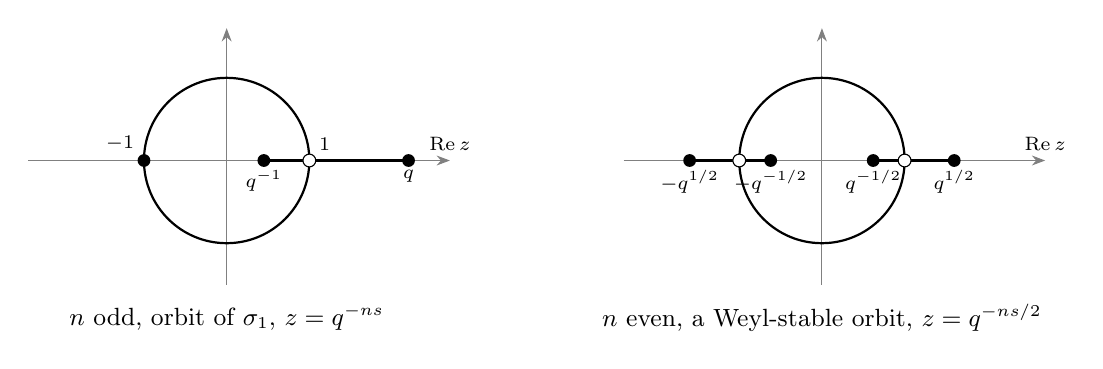
\begin{tikzpicture}[scale=1.05,>=Stealth]
% n odd, orbit of sigma_1
\begin{scope}
\draw[->,gray] (-2.4,0)--(2.7,0) node[above,black] {\scriptsize $\re z$};
\draw[->,gray] (0,-1.5)--(0,1.6);
\draw[thick] (0,0) circle (1);
\draw[very thick] (0.45,0)--(1,0);
\draw[very thick] (1,0)--(2.2,0);
\fill (0.45,0) circle (2.2pt) node[below] {\scriptsize $q^{-1}$};
\fill (2.2,0) circle (2.2pt) node[below] {\scriptsize $q$};
\draw[fill=white] (1,0) circle (2.2pt);
\node[above right] at (1,0) {\scriptsize $1$};
\fill (-1,0) circle (2.2pt) node[above left] {\scriptsize $-1$};
\node at (0,-1.9) {\small $n$ odd, orbit of $\sigma_1$, $z=q^{-ns}$};
\end{scope}
% n even
\begin{scope}[xshift=7.2cm]
\draw[->,gray] (-2.4,0)--(2.7,0) node[above,black] {\scriptsize $\re z$};
\draw[->,gray] (0,-1.5)--(0,1.6);
\draw[thick] (0,0) circle (1);
\draw[very thick] (0.62,0)--(1.6,0);
\draw[very thick] (-0.62,0)--(-1.6,0);
\fill (0.62,0) circle (2.2pt) node[below] {\scriptsize $q^{-1/2}$};
\fill (1.6,0) circle (2.2pt) node[below] {\scriptsize $q^{1/2}$};
\fill (-0.62,0) circle (2.2pt) node[below] {\scriptsize $-q^{-1/2}$};
\fill (-1.6,0) circle (2.2pt) node[below] {\scriptsize $-q^{1/2}$};
\draw[fill=white] (1,0) circle (2.2pt);
\draw[fill=white] (-1,0) circle (2.2pt);
\node at (0,-1.9) {\small $n$ even, a Weyl-stable orbit, $z=q^{-ns/2}$};
\end{scope}
\end{tikzpicture}
\caption{The Weyl-stable orbits of unramified twists that contain reducible points, for
$p\nmid n$, in the coordinate $z$.  The Weyl group acts by $z\mapsto z^{-1}$.  The circle
is the unitary principal series.  The thick segments are the complementary series, drawn
with their mirror images under $W$.  Black dots are reducible points and white dots are
irreducible Weyl-fixed points.  For $n$ odd and $p$ odd there is a second Weyl-stable
orbit, through the two ramified quadratic characters, with reducible points at $z=\pm1$
and no complementary series.  For $n$ even and $p$ odd there are two orbits of the kind
shown.}\label{fig:dual}
\end{figure}

\begin{xexample}\label{ex:two-pictures}
The left picture in Figure~\ref{fig:dual} is the picture for $SL(2,F)$ itself, with
$z=q^{-s}$.  The right picture is the picture for $PGL(2,F)$, where $I(\chi)$ is reducible
at $\chi^2=|\cdot|^{\pm1}$, that is, at $\chi=|\cdot|^{\pm1/2}$ and at its twist by the
unramified quadratic character.  So the reducibility pattern of the $n$-fold cover of
$SL(2,F)$ is that of $SL(2,F)$ for $n$ odd and that of $PGL(2,F)$ for $n$ even.  This is
consistent with the dual groups attached to these covers, for which see \cite{GSS23} and
its references.  See Problem~\ref{prob:shimura}.
\end{xexample}
%======================================================================
\section{The Fourier Transform}\label{sec:fourier}

This section introduces the transforms studied in the rest of the paper.  The
operator-valued transform sends a test function to the family of operators $\pi(f)$.  The
trace transform sends it to the family of numbers $\tr\pi(f)$.  The second is the relevant
object for invariant harmonic analysis.  The two have different kernels.

For $f\in C_c^\infty(\bG)$ and a genuine admissible representation $\pi$ the
\emph{operator-valued Fourier transform} of $f$ at $\pi$ is
\[
\pi(f)=\int_{\bG}f(x)\pi(x)\,dx .
\]

\begin{lemma}[\proved]\label{lem:conv}
If $f,g\in C_c^\infty(\bG)$ then $\pi(f*g)=\pi(f)\pi(g)$.
\end{lemma}
\begin{proof}
This is Fubini's theorem and the invariance of Haar measure.  The convolution of two
genuine functions is genuine.
\end{proof}

Let $\bG'=\{(g,\zeta)\in\bG\mid g\ \text{has distinct eigenvalues}\}$, the \emph{regular
set}.  Every element of the regular set is semisimple.

\begin{lemma}[Harish-Chandra, Howe; for covers \cite{Li12}; \cited]\label{lem:character}
Let $\pi$ be a genuine admissible representation of finite length.  There is a locally
constant function $\Theta_\pi$ on $\bG'$, locally integrable on $\bG$, with
$\Theta_\pi(\zeta x)=\zeta\,\Theta_\pi(x)$, such that
\[
\tr\pi(f)=\int_{\bG}\Theta_\pi(x)f(x)\,dx\qquad\text{for all }f\in C_c^\infty(\bG).
\]
\end{lemma}
The number $\Theta_\pi(f)=\tr\pi(f)$ is called the \emph{Fourier transform} of $f$ at
$\pi$, and the function $\Theta_\pi$ is the \emph{character} of $\pi$.  The regularity of
characters of covering groups is established in \cite[\S4]{Li12}.  The 1994 manuscript
sketched a proof along the lines of \cite[Corollary~4.8.2]{Si79}.  By
Lemma~\ref{lem:splittings}(c) the cover splits over every sufficiently small compact open
subgroup $K'$ of $G$.  One identifies the representations of $K'$ with the representations
of $\overline{K'}$ that are trivial on $\mu_n$, and replaces Howe's finiteness theorem
\cite[Theorem~4.8.1]{Si79} by the following statement.

\begin{lemma}[\cited]\label{lem:howe}
Let $T$ be a Cartan subgroup of $G$ and let $\omega\subset T\cap G'$ be compact.  There is a
compact open subgroup $K_1\subset G$ over which the cover splits, with the following
property.  For every compact open subgroup $K_2$ over which the cover splits and every
irreducible representation $\mathbf d_2$ of $K_2$, the set of irreducible representations
$\mathbf d_1$ of $K_1$ such that $\bG$ intertwines $\mathbf d_1$ with $\mathbf d_2$ and
$\omega$ intertwines $\mathbf d_1$ with itself is finite.
\end{lemma}
\unverified{This lemma is the 1994 formulation.  Its proof for covers was not written out
there and was not checked here.  We rely on \cite{Li12} for Lemma~\ref{lem:character}.}

\begin{xproposition}[The trace descends to the cocenter; \proved]\label{prop:cocenter}
Let $\pi$ be a genuine admissible representation.  Then $\tr\pi(f*g-g*f)=0$ and
$\tr\pi(f-f^y)=0$ for $f,g\in C_c^\infty(\bG)$ and $y\in\bG$, where
$f^y(x)=f(y^{-1}xy)$.
\end{xproposition}
\begin{proof}
The first identity follows from Lemma~\ref{lem:conv} and the cyclicity of the trace of
finite-rank operators.  For the second, $\pi(f^y)=\pi(y)\pi(f)\pi(y)^{-1}$ because $\bG$ is
unimodular.
\end{proof}

\begin{xexample}\label{ex:kernels}
Let $f$ be supported in a small neighborhood of a non-central element and let $y$ be such
that $f^y$ has disjoint support.  Then $f-f^y\ne0$ has trace zero in every representation,
while $\pi(f-f^y)\ne0$ for suitable $\pi$.  So the trace transform has a large kernel and
the operator-valued transform does not.  A second example is special to covers.  Let
$a\in\bA\setminus\bZ$ and choose $b\in\bA$ with $bab^{-1}=\zeta a$, $\zeta\ne1$.  Let $f$ be
genuine, supported on $\mu_nU$ for a small neighborhood $U$ of $a$ that is stable under
$x\mapsto\zeta^{-1}bxb^{-1}$, and equal to $1$ on $U$.  Then
$f^{b^{-1}}(x)=f(bxb^{-1})=\zeta^{-1}f(x)$.  So $(1-\zeta^{-1})f$, and hence $f$ itself, lies in
the kernel of every trace.  Genuine invariant distributions do not see such elements.
\end{xexample}

\subsection{The Schwartz space and the tempered dual}\label{subsec:schwartz}

This subsection defines the Schwartz space, the orbital integrals on the split torus, and
tempered representations.

Let $\|g\|=\max(|a|,|b|,|c|,|d|)$ for $g=\begin{pmatrix}a&b\\c&d\end{pmatrix}$ and
$\sigma(g)=\log\|g\|\ge0$.  Extend $\delta_B$ to $G$ by $\delta_B(buk)=\delta_B(b)$.
Harish-Chandra's function is
\[
\Xi(x)=\int_K\delta_B(kx)^{1/2}\,dk .
\]
It is bi-$K$-invariant, and there are constants $c_1,c_2,r_0>0$ with
\[
c_1\,q^{-m}\le\Xi(h(\vp^m))\le c_2\,q^{-m}(1+m)^{r_0}\qquad(m\ge0).
\]
Both $\Xi$ and $\sigma$ are pulled back to $\bG$.  For a compact open subgroup
$K'\subset\bG$ with $K'\cap\mu_n=1$ let $\calC_{K'}(\bG)$ be the space of genuine
bi-$K'$-invariant functions $f$ on $\bG$ with
\[
\upsilon_r(f)=\sup_{x\in\bG}|f(x)|\,\frac{(1+\sigma(x))^r}{\Xi(x)}<\infty\qquad\text{for all }r>0 .
\]
It is a Fr\'echet space for the seminorms $\upsilon_r$.  Let
$\calC(\bG)=\bigcup_{K'}\calC_{K'}(\bG)$ with the locally convex inductive limit topology.
This is the \emph{Schwartz space} of $\bG$.  Compact support is not part of the definition.

\begin{lemma}[Harish-Chandra; for covers \cite{Li12}; \cited]\label{lem:schwartz-alg}
(1) $C_c^\infty(\bG)\subset\calC(\bG)\subset L^2(\bG)$.
(2) $\calC(\bG)$ is an algebra under convolution.
\end{lemma}
The absolute value of a genuine function is a function on $G$.  So estimates such as (1)
reduce to the linear case \cite[\S4.4]{Si79}.

\begin{xexample}
On the torus the analogous space is $\calC(\bZ)$: the genuine functions on $\bZ$ that are
invariant under an open subgroup and satisfy $|\phi(z)|\ll_r(1+|v(t)|)^{-r}$ for $z$ over
$h(t)$.  A function in $C_c^\infty(\bZ)$ has only finitely many nonzero ``Fourier
coefficients'' in the variable $v(t)$.  A function in $\calC(\bZ)$ has rapidly decreasing
ones.
\end{xexample}

Let $D(h(a))=\det(1-\Ad(h(a)))|_{\mathfrak g/\mathfrak a}=(1-a^2)(1-a^{-2})=-(a-a^{-1})^2$,
pulled back to $\bG'$ through conjugation and $\pr$.  For $t\in\bG'$ let
$\bG_t=\Cent(t,\bG)$.  This need not be the preimage of the centralizer of $\pr(t)$.  The
\emph{orbital integral} of $f\in C_c^\infty(\bG)$ is
\begin{equation}\label{eq:orbital}
F_f^{T}(t)=|D(t)|^{1/2}\int_{\bG_t\backslash\bG}f(x^{-1}tx)\,dx .
\end{equation}
It converges by \cite{HC70}.  For linear groups the image of the orbital integrals is
characterized in \cite{Vi81}.  For regular $a\in\bA$ define also
\begin{equation}\label{eq:orbital-Z}
F_f^{\bZ}(a)=|D(a)|^{1/2}\int_{\bZ\backslash\bG}f(x^{-1}ax)\,dx .
\end{equation}

\begin{lemma}[\proved]\label{lem:vanish}
For $f\in C_c^\infty(\bG)$ and regular $a\in\bA\setminus\bZ$ we have $F_f^{\bZ}(a)=0$.
\end{lemma}
\begin{proof}
Split the integral into an integral over $\bA\backslash\bG$ and a finite sum over
$\bZ\backslash\bA$.  For $b\in\bA$ put $c(b)=a^{-1}b^{-1}ab\in\mu_n$.  The map $b\mapsto c(b)$ is
a homomorphism, trivial on $\bZ$ and nontrivial because $a$ is not central.  Since $f$ is
genuine, $f(x^{-1}b^{-1}abx)=c(b)^{-1}f(x^{-1}ax)$.  The inner sum is $f(x^{-1}ax)$ times the
sum of a nontrivial character of a finite group.
\end{proof}

\paragraph{The Abel transform.}  For $f\in C_c^\infty(\bG)$ put
\begin{equation}\label{eq:fK}
f^{K}(x)=\int_{K}f(\tilde k^{-1}x\tilde k)\,dk,
\end{equation}
where $\tilde k$ is any lift of $k$, and for $a\in\bA$
\begin{equation}\label{eq:fB}
f^{(B)}(a)=\delta_B(a)^{1/2}\int_Nf^{K}(a\tilde u)\,du,\qquad \Phi_f=f^{(B)}|_{\bZ}.
\end{equation}
The function $f^{(B)}$ is genuine, locally constant and compactly supported on $\bA$.  For
regular $z\in\bZ$ over $h(t)$ the centralizer is $\bA$, and the substitution
$\tilde u^{-1}z\tilde u=z\,\widetilde{u((1-t^{-2})x)}$ gives
\begin{equation}\label{eq:Phi-orbital}
\Phi_f(z)=|D(z)|^{1/2}\int_{\bA\backslash\bG}f(x^{-1}zx)\,dx=F_f^{T}(z),
\end{equation}
with the quotient measure $du\,dk$.  So $\Phi_f$ is the locally constant extension of the
split orbital integral to all of $\bZ$.  It satisfies $\Phi_f(\wt z\wt^{-1})=\Phi_f(z)$.  Let
$C_c^\infty(\bZ)^W$ be the space of genuine functions in $C_c^\infty(\bZ)$ with this
invariance, and define $\calC(\bZ)^W$ similarly.

\begin{lemma}[\proved\ for (1); (2) is \cited\ and \cond]\label{lem:orbital-image}
(1) Assume $p\nmid2n$.  The map $f\mapsto\Phi_f$ is a surjection
$C_c^\infty(\bG)\to C_c^\infty(\bZ)^W$.

(2) The map $f\mapsto\Phi_f$ extends to a continuous map
$\calC(\bG)\to\calC(\bZ)^W$.  It is surjective if Theorem~\ref{thm:PWt}(b) holds.
\end{lemma}
\begin{proof}
(1) This is \cite[Theorem on the image of the split orbital integral]{JoUD}.  We recall
the argument.  The map $(\bA x,z)\mapsto x^{-1}zx$ from
$(\bA\backslash\bG)\times\bZ_{reg}$ to $\bG$ is a local homeomorphism, with fibers
$\{(\bA x,z),(\bA\wt x,\wt z\wt^{-1})\}$.  Let $\phi\in C_c^\infty(\bZ)^W$ vanish near the
singular set, and let $\alpha$ be the characteristic function of $\bA K^*$ in
$\bA\backslash\bG$.  The function
$f(x^{-1}zx)=\phi(z)(\alpha(\bA x)+\alpha(\bA\wt x))/(2|D(z)|^{1/2})$, extended by zero, is
well defined, genuine, locally constant and compactly supported, and $\Phi_f=\phi$.

The singular elements of $\bZ$ lie over $\pm1$.  For $\varepsilon=\pm1$ let
$z_\varepsilon=(\varepsilon,1)$, which is central in $\bG$, and for $m\ge1$ let
$f_{\varepsilon,m}$ be the genuine function supported on $\mu_nz_\varepsilon s(K_m)$ with
$f_{\varepsilon,m}(z_\varepsilon s(k))=1$.  Since $K_m$ is normal in $K$ we have
$f_{\varepsilon,m}^K=f_{\varepsilon,m}$.  By \eqref{eq:fB},
$\Phi_{f_{\varepsilon,m}}$ is $q^{-m}$ times the genuine function supported on
$\mu_nz_\varepsilon\hl(U_m)$ with value $1$ on $z_\varepsilon\hl(U_m)$.  Here
$U_m\subset F^{\times\nu}$ because $p\nmid\nu$.  The two supports are disjoint because $p$ is
odd.  Given $\phi\in C_c^\infty(\bZ)^W$, choose $m$ so large that $\phi$ is constant on
$z_\varepsilon\hl(U_m)$.  Then
$\phi-\sum_\varepsilon q^m\phi(z_\varepsilon)\Phi_{f_{\varepsilon,m}}$ vanishes near the
singular set, and the first step applies.

(2) Since $|f|$ is a function on $G$, the continuity is Harish-Chandra's estimate for the
constant term along $B$ \cite[\S4.4]{Si79}.  The surjectivity is the statement that every
$W$-invariant smooth function on the unitary characters of $\bZ$, supported on finitely
many circles, is the trace transform of a Schwartz function.
\end{proof}

\begin{xexample}\label{ex:Phi-eK}
Assume $p\nmid 2n$ and let $e_K$ be the genuine function supported on $\mu_nK^*$ with
$e_K(s(k))=1$.  Then $\Phi_{e_K}$ is the genuine function supported on
$\mu_n\hl(\OF^{\times\nu})$ with value $1$ on $\hl(\OF^{\times\nu})$.  Indeed $z\tilde u\in\mu_nK^*$
forces $z$ to lie over $h(\OF^\times)$ and $u\in N\cap K$.
\end{xexample}

We call a distribution on $C_c^\infty(\bG)$ \emph{tempered} if it extends continuously to
$\calC(\bG)$.  A locally constant function $h$ on $\bG$ with $h(\zeta x)=\zeta h(x)$ is
\emph{tempered} if the distribution $f\mapsto\int_{\bG}f(x)h(x)\,dx$ is tempered.  An
admissible representation $\pi$ is \emph{tempered} if every matrix coefficient of $\pi$ is
tempered.

\begin{lemma}[Analog of {\cite[Lemma~4.5.2]{Si79}}; \cited]\label{lem:tempered-char}
A class $\pi\in\Pia$ is tempered if and only if the distribution $f\mapsto\Theta_\pi(f)$
extends continuously to $\calC(\bG)$.
\end{lemma}
For $p\nmid n$ this can be checked on the list of Theorem~\ref{thm:unitary-dual}, using
the Jacquet modules.  In general it is part of the theory of \cite[\S2]{Li12}.

\begin{proposition}[Conjecture 4.8 of 1994; \cited]\label{prop:temp-unitary}
(a) A genuine irreducible tempered representation of $\bG$ is unitarizable.
(b) A genuine square-integrable representation of $\bG$ is tempered.
\end{proposition}
Part (b) follows from Casselman's criteria for covers \cite{BJ13}.  Part (a) holds because
an irreducible tempered representation is a subrepresentation of a representation induced
from a square-integrable one \cite[\S2]{Li12}.  For $p\nmid n$ both are visible in
Theorem~\ref{thm:unitary-dual}.

\subsection{Character calculations}\label{subsec:characters}

We compute the characters of the principal series and use them to express the trace
transform by the Abel transform.  Let $S$ be a set of representatives of the conjugacy
classes of Cartan subgroups of $G$, with $A\in S$.  For $T\in S$ let $W_T=N_G(T)/T$.

\begin{lemma}[Weyl integration formula {\cite[p.~198]{Si79}}; \cited]\label{lem:weyl-int}
For $f\in C_c^\infty(G)$,
\[
\int_Gf(g)\,dg=\sum_{T\in S}\frac1{|W_T|}\int_T|D(t)|^{1/2}F_f^T(t)\,dt,\qquad
F_f^T(t)=|D(t)|^{1/2}\int_{T\backslash G}f(x^{-1}tx)\,dx .
\]
\end{lemma}
Note that $F_f^T(t)=F_f^T(t^w)$ for $w\in W_T$.  On the cover the same formula holds for
$\mu_n$-invariant integrands.  A function $\Theta$ on $\bG'$ that is invariant under
conjugation and satisfies $\Theta(\zeta x)=\zeta\Theta(x)$ vanishes at every regular
$a\in\bA\setminus\bZ$, because $a$ is conjugate to $\zeta a$ for some $\zeta\ne1$.  If such
a $\Theta$ is supported on the conjugates of $\bZ$, then for genuine $f$
\begin{equation}\label{eq:weyl-cover}
\int_{\bG}f(x)\Theta(x)\,dx=\frac12\int_{A^\nu}|D(z)|^{1/2}\,\Theta(z)\,\Phi_f(z)\,dz,
\end{equation}
where $A^\nu=h(F^{\times\nu})$ and the integrand is evaluated at any lift of $z$.

\subsubsection{Principal series}

\begin{lemma}[\proved]\label{lem:ps-character}
Let $\sigma\in\Pi(\bA)$, with no restriction on $p$.  Then for $f\in C_c^\infty(\bG)$
\begin{equation}\label{eq:trace-ps}
\tr I(\sigma)(f)=\int_A f^{(B)}(a)\,\tr\sigma(a)\,da=d_\sigma\int_{A^\nu}\Phi_f(z)\,\omega_\sigma(z)\,dz .
\end{equation}
The character of $I(\sigma)$ is given on the regular set by
\[
\Theta_{I(\sigma)}(x)=\begin{cases}
d_\sigma\,\dfrac{\omega_\sigma(z)+\omega_\sigma(\wt z\wt^{-1})}{|D(z)|^{1/2}},& x\ \text{conjugate to a regular}\ z\in\bZ,\\[8pt]
0,& \text{otherwise}.
\end{cases}
\]
Here $|D(z)|^{1/2}=|t-t^{-1}|$ for $z$ over $h(t)$.
\end{lemma}
\begin{proof}
Let $\varphi\in I(\sigma)$ and $k\in\bK$.  With $dg=da\,du\,dk$ for $g=auk$,
\begin{align*}
(I(\sigma)(f)\varphi)(k)&=\int_{\bG}f(k^{-1}x)\varphi(x)\,dx\\
&=\int_K\Bigl(\int_A\int_N\delta_B(a)^{1/2}f(k^{-1}a\tilde uk_1)\,\sigma(a)\,du\,da\Bigr)\varphi(k_1)\,dk_1 .
\end{align*}
The restriction of $\varphi$ to $\bK$ identifies $I(\sigma)$ with a space of
$V_\sigma$-valued functions on $\bK$, and $I(\sigma)(f)$ is an integral operator with the
kernel in parentheses.  Its trace is the integral of the trace of the kernel over the
diagonal:
\begin{equation}\label{eq:trace-kernel}
\tr I(\sigma)(f)=\int_A\delta_B(a)^{1/2}\tr\sigma(a)\int_N\int_Kf(k^{-1}a\tilde uk)\,dk\,du\,da .
\end{equation}
This is the first equality in \eqref{eq:trace-ps}.  The second follows from
Corollary~\ref{cor:torus-trace}.  By the Weyl invariance of $\Phi_f$,
\[
\tr I(\sigma)(f)=\frac{d_\sigma}2\int_{A^\nu}\Phi_f(z)\bigl(\omega_\sigma(z)+\omega_\sigma(\wt z\wt^{-1})\bigr)dz .
\]
Comparing with \eqref{eq:weyl-cover} and using Lemma~\ref{lem:orbital-image}(1), or its
first step, which holds for every $p$, we obtain the character on the conjugates of
$\bZ_{reg}$.  A function $f$ supported on the regular elliptic set, or near a regular
$a\in\bA\setminus\bZ$, has $\Phi_f=0$, so the character vanishes there.
\end{proof}

In terms of a genuine character $\mu$ of $\bC$ with $\sigma=\Ind_{\bC}^{\bA}\mu$,
Corollary~\ref{cor:torus-trace} gives
\begin{equation}\label{eq:trace-mu}
\tr\sigma(a)=\sum_{h\in\bA/\bC}\mu^h(a)\quad(a\in\bC),\qquad
\Theta_{I(\sigma)}(f)=\sum_{h\in\bA/\bC}\int_{h(C)}f^{(B)}(a)\,\mu^h(a)\,da .
\end{equation}
For $\varphi\in C_c^\infty(\bZ)$ and a genuine character $\omega$ of $\bZ$ we write
\begin{equation}\label{eq:mellin}
\varphi^\wedge(\omega)=\int_{A^\nu}\varphi(z)\,\omega(z)\,dz .
\end{equation}
So $\Theta_{I(\sigma)}(f)=d_\sigma\,\Phi_f^\wedge(\omega_\sigma)$.  If $z$ over
$h(\vp^{\nu k}u)$ is written as $\hl(\vp^\nu)^k\hl(u)$ up to an element of $\mu_n$, then
\eqref{eq:mellin} becomes a finite sum $\sum_kc_k\,\omega(\hl(\vp^\nu))^k$, a Laurent
polynomial in $\omega(\hl(\vp^\nu))$.  These formulas extend to $f\in\calC(\bG)$ when $\sigma$
is unitary.

\begin{xexample}\label{ex:trace-eK}
For $p\nmid2n$ and $f=e_K$ (Example~\ref{ex:Phi-eK}), formula \eqref{eq:trace-ps} gives
$\tr I(\sigma)(e_K)=d_\sigma\vol(\OF^{\times\nu})$ if $\sigma$ is unramified and $0$ otherwise.
With $\vol(\OF^\times)=1$ this is $d_\sigma/\nu=1$, the dimension of $I(\sigma)^{K^*}$
(Lemma~\ref{lem:spherical}).
\end{xexample}

\subsubsection{Reducible principal series}
Let $n$ be odd and let $I(\sigma)=\pi^+\oplus\pi^-$ be reducible with $\sigma$ unitary.  The
sum $\Theta_{\pi^+}+\Theta_{\pi^-}$ is given by Lemma~\ref{lem:ps-character}.  The difference
is supported on the elliptic set and on the singular set, by the same lemma applied to the
normalized intertwining operator.  For $n=1$ it is the well-known unstable character
attached to a quadratic extension.  For odd $n>1$ it is not known explicitly.  Some
information can be obtained by global means \cite{Jo88,Fl80}, and the Whittaker dimensions
of $\pi^\pm$ are computed in \cite{Sz24}.

\subsubsection{Complementary series}
These representations are not tempered.  Their characters are given by
Lemma~\ref{lem:ps-character}, and $|D(z)|^{1/2}\Theta(z)$ grows like $|t|^{-s}$ as
$|t|\to0$.

\subsubsection{The non-tempered representation}
The representation $\pi_{nt}$ is the quotient of $I(\sigma_0\otimes\eta_{1/n})$ by a
special representation.  Its character is $\Theta_{I(\sigma)}-\Theta_{\pi_{sp}}$.

\subsubsection{Square-integrable representations}
These are tempered and occur discretely.  For the depth-zero cuspidal representations of
Example~\ref{ex:depth-zero} the characters on the unramified elliptic tori are computed
in \cite{JoCh}.  The character of $\pi_{sp}$ on the elliptic set is not known explicitly
for $n>1$ (Problem~\ref{prob:characters}).

%======================================================================
\section{The image of the Fourier transform}\label{sec:image}

This section describes the image of the trace transform in three settings.  We first
treat the torus and the full principal series, where everything is explicit.  We then
state the admissible, the unitary and the tempered Paley--Wiener theorems on the
irreducible duals.  For each we separate what is proved here from what is cited.

\paragraph{Parameters.}  The set $\Pi(\bA)$ is identified with the genuine characters of
$\bZ$.  It is a disjoint union of orbits $\fX$ under the twists $\sigma\mapsto\sigma\otimes\eta_s$.
Each orbit has the coordinate $z=q^{-\nu s}$ relative to a base point, and is a copy of
$\C^\times$.  The unitary classes in $\fX$ form the circle $|z|=1$, when the base point is
unitary.  A function on $\fX$ is a \emph{Laurent polynomial} if it is a polynomial in $z$
and $z^{-1}$.  This notion does not depend on the base point.  The Weyl group permutes the
orbits.

Recall the Mellin transform on $F^\times$:
$\varphi^\wedge(\omega)=\int_{F^\times}\omega(x)\varphi(x)\,d^\times x$ for a character
$\omega$ of $F^\times$.  The characters of $F^\times$ form a disjoint union of copies of
$\C^\times$, indexed by the characters of $\OF^\times$, with coordinate $\omega(\vp)$.

\begin{lemma}[\proved]\label{lem:PW-Fx}
The image of $C_c^\infty(F^\times)$ under $\varphi\mapsto\varphi^\wedge$ is the space of
functions on the characters of $F^\times$ that vanish outside finitely many components and
are Laurent polynomials in $\omega(\vp)$ on each.  Restricted to the unitary characters,
these are the functions that vanish outside finitely many circles and are trigonometric
polynomials on each.
\end{lemma}
\begin{proof}
Write $\varphi=\sum_{k}\varphi_k$ with $\varphi_k$ supported on $\vp^k\OF^\times$, a finite
sum.  Each $\varphi_k(\vp^k\,\cdot\,)$ is a finite linear combination of characters of
$\OF^\times$, by Fourier analysis on the compact group $\OF^\times$ and local constancy.
The transform of $\vp^ku\mapsto\lambda(u)^{-1}$ is $\omega(\vp)^k$ on the component of
$\lambda$ and $0$ elsewhere.  Conversely every such function arises.  See
\cite[pp.~43--44]{Ta75}.
\end{proof}

\begin{lemma}[\proved]\label{lem:PW-A}
The same description holds for $C_c^\infty(A)$, with $A\cong F^\times$ via $h$.
\end{lemma}

\begin{lemma}[\proved]\label{lem:PW-Z}
The image of the genuine functions in $C_c^\infty(\bZ)$ under
$\varphi\mapsto\varphi^\wedge$ of \eqref{eq:mellin} is the space of functions on $\Pi(\bA)$
that vanish outside finitely many orbits $\fX$ and are Laurent polynomials on each.  The
map is injective.
\end{lemma}
\begin{proof}
The group $\bZ$ is abelian, and $\bZ/\mu_n\cong F^{\times\nu}$ is isomorphic to
$\Z\times(\text{compact})$.  The genuine characters of $\bZ$ form a torsor under the
characters of $F^{\times\nu}$.  After multiplying by a fixed genuine character the
statement becomes Lemma~\ref{lem:PW-Fx} for $F^{\times\nu}$, whose proof applies to any
group of this form.
\end{proof}

As a consequence of Lemmas~\ref{lem:ps-character}, \ref{lem:PW-Z} and
\ref{lem:orbital-image}(1) we obtain the image of the trace transform on full principal
series.

\begin{lemma}[Paley--Wiener theorem for principal series; \proved]\label{lem:PWps}
For $f\in C_c^\infty(\bG)$ let $f^\wedge_{ps}(\sigma)=\Theta_{I(\sigma)}(f)$, $\sigma\in\Pi(\bA)$.
\begin{enumerate}[label=(\alph*),leftmargin=*,itemsep=1pt]
\item For every $p$, the function $f^\wedge_{ps}$ vanishes outside finitely many orbits, is a
Laurent polynomial on each orbit, and satisfies $f^\wedge_{ps}(\sigma^w)=f^\wedge_{ps}(\sigma)$.
\item Assume $p\nmid2n$.  Every function on $\Pi(\bA)$ with these three properties is
$f^\wedge_{ps}$ for some $f\in C_c^\infty(\bG)$.
\end{enumerate}
Restricted to $\Pi_u(\bA)$, the image consists of the $W$-invariant functions that vanish
outside finitely many circles and are trigonometric polynomials on each.
\end{lemma}
\begin{proof}
By \eqref{eq:trace-ps}, $f^\wedge_{ps}(\sigma)=d_\sigma\Phi_f^\wedge(\omega_\sigma)$, and
$d_\sigma$ does not depend on $\sigma$.  The Mellin transform intertwines the action of
$\wt$ on $\bZ$ with $\sigma\mapsto\sigma^w$.  So (a) follows from Lemma~\ref{lem:PW-Z} and the
invariance of $\Phi_f$, and (b) from Lemma~\ref{lem:orbital-image}(1).
\end{proof}

\begin{xexample}\label{ex:PWps}
Let $p\nmid 2n$ and let $\fX$ be the orbit of an unramified Weyl-fixed $\sigma_0$, with
$z=q^{-\nu s}$.  The Weyl group acts by $z\mapsto z^{-1}$.  The functions $1$ and
$z^k+z^{-k}$, $k\ge1$, extended by zero to the other orbits, are trace transforms.  The
function $1$ is the transform of $e_K$ by Example~\ref{ex:trace-eK}.  The function $z$
alone is not a trace transform.
\end{xexample}

Next we consider $f\in\calC(\bG)$, for which $\Phi_f\in\calC(\bZ)^W$.

\begin{lemma}[\proved]\label{lem:SPW-Fx}
The image of $\calC(F^\times)$ under the Mellin transform on the unitary characters is the
space of functions that vanish outside finitely many circles and are smooth on each.
Equivalently, on each circle they are given by a trigonometric series that converges
absolutely together with all of its derivatives.
\end{lemma}
\begin{proof}
A function in $\calC(F^\times)$ is invariant under some $U_m$ and its components
$\varphi_k$ decay faster than any power of $|k|$.  The Fourier coefficients of a function
on the circle decay rapidly if and only if the function is smooth.
\end{proof}

\begin{lemma}[\proved]\label{lem:SPW-Z}
The image of the genuine functions in $\calC(\bZ)$ under \eqref{eq:mellin}, on the unitary
classes, is the space of functions on $\Pi_u(\bA)$ that vanish outside finitely many
circles and are smooth on each.
\end{lemma}

\begin{lemma}[necessity \proved; surjectivity \cond]\label{lem:SPWps}
For $f\in\calC(\bG)$ the function $\sigma\mapsto\Theta_{I(\sigma)}(f)$ on $\Pi_u(\bA)$ is
$W$-invariant, vanishes outside finitely many circles and is smooth on each.  Every such
function arises if Theorem~\ref{thm:PWt}(b) holds.
\end{lemma}
\begin{proof}
The first statement follows from Lemma~\ref{lem:orbital-image}(2), formula
\eqref{eq:trace-ps} for $\calC(\bG)$ and Lemma~\ref{lem:SPW-Z}.
\end{proof}

\subsection{Admissible Paley--Wiener Theorem for smooth functions}\label{subsec:PWad}

This subsection gives the analog for $\bG$ of the theorem of Bernstein, Deligne and
Kazhdan \cite{BDK86}.  The trace transform of $f\in C_c^\infty(\bG)$ is the function
$\hat f(\pi)=\Theta_\pi(f)$ on $\Pia$.

For a function $h$ on $\Pia$ and $\sigma\in\Pi(\bA)$ put
\[
h^{ind}(\sigma)=\sum_{\pi\in\JH(I(\sigma))}h(\pi),
\]
the sum over the irreducible constituents of $I(\sigma)$.  The constituents are pairwise
inequivalent.  A \emph{component} of $\Pia$ is either a single cuspidal class or the set of
constituents of the $I(\sigma)$, $\sigma\in\fX\cup w\fX$, for an orbit $\fX$.

\begin{xdefinition}\label{def:PWad}
The \emph{admissible Paley--Wiener space} $PW_{ad}(\bG)$ is the space of functions $h$ on
$\Pia$ such that
\begin{enumerate}[label=(PW\arabic*),leftmargin=*,itemsep=1pt]
\item $h$ vanishes outside finitely many components,
\item for each orbit $\fX$ the function $h^{ind}|_{\fX}$ is a Laurent polynomial.
\end{enumerate}
\end{xdefinition}
The function $h^{ind}$ is automatically $W$-invariant, because $I(\sigma)$ and $I(\sigma^w)$
have the same constituents.  Condition (PW2) is the precise meaning of the phrase
``$h$ is regular on $\Pia$, regarded as a complex algebraic variety'' of the 1994
manuscript.  At a reducible point it constrains only the sum of the two values of $h$.

\begin{theorem}[Admissible Paley--Wiener theorem]\label{thm:PWad}
Let $f\mapsto\hat f$ be the trace transform on $C_c^\infty(\bG)$.
\begin{enumerate}[label=(\alph*),leftmargin=*,itemsep=1pt]
\item (Necessity; \proved.)  For every $p$ and every $f$ we have $\hat f\in PW_{ad}(\bG)$.
\item (Surjectivity up to the reducible points; \proved.)  Assume $p\nmid2n$.  Let $P$ be a
$W$-invariant function on $\Pi(\bA)$ that vanishes outside finitely many orbits and is a
Laurent polynomial on each, and let $c$ be a finitely supported function on $\Pi_c(\bG)$.
Then there is $f\in C_c^\infty(\bG)$ with $\hat f^{\,ind}=P$ and $\hat f|_{\Pi_c(\bG)}=c$.
\item (Surjectivity; \cited.)  The trace transform maps $C_c^\infty(\bG)$ onto
$PW_{ad}(\bG)$.
\item (Kernel; \cited.)  The kernel of the trace transform is the span of the functions
$f-f^y$.
\end{enumerate}
\end{theorem}
\begin{proof}
(a) Let $f$ be bi-invariant under a compact open subgroup $K'$ with $K'\cap\mu_n=1$.  If
$\Theta_\pi(f)\ne0$ then $\pi$ has a nonzero $K'$-fixed vector.  Only finitely many
cuspidal classes have one, by the Bernstein decomposition and uniform admissibility
\cite[Theorems~3.4 and 3.9]{KS23}.  If $I(\sigma)$ has a $K'$-fixed vector then, by the
decomposition of $\bG$ into finitely many double cosets $\bB xK'$, the character
$\omega_\sigma$ is trivial on $\bZ\cap xK'x^{-1}$ for one of finitely many $x$.  This
restricts $\sigma$ to finitely many orbits.  So (PW1) holds.  The trace is additive on
composition series, so $\hat f^{\,ind}(\sigma)=\Theta_{I(\sigma)}(f)$, and (PW2) is
Lemma~\ref{lem:PWps}(a).

(b) By Lemma~\ref{lem:PWps}(b) there is $f_0$ with $\hat f_0^{\,ind}=P$.  The function
$\hat f_0$ is nonzero at only finitely many cuspidal classes.  By Lemma~\ref{lem:pseudo}
we can add a finite linear combination of pseudo-coefficients $f_\pi$ to correct the
values on $\Pi_c(\bG)$ without changing $\hat f_0^{\,ind}$.

(c) This is the trace Paley--Wiener theorem of \cite{BDK86} for the group $\bG$.  Li
states that the arguments of \cite{BDK86} adapt to covering groups
\cite[\S3.4]{Li14}.  The tools used in \cite{BDK86} are available for covers by
\cite{KS23}.  In the present rank-one situation a function $h$ on $\Pia$, extended
additively to the Grothendieck group, is a ``good form'' in the sense of \cite{BDK86}
exactly when it satisfies (PW1) and (PW2).  Indeed $\bG$ has no nontrivial unramified
characters, so the regularity condition is empty for the Levi subgroup $\bG$ and is
(PW2) for the Levi subgroup $\bA$.

(d) This is \cite[Th\'eor\`eme~5.8.10]{Li12}.
\end{proof}

\unverified{We did not find a written proof of the theorem of \cite{BDK86} for covering
groups.  Part (c) rests on Li's statement.  By (b), what (c) adds is the following
\emph{separation property}: for each $\sigma$ with $I(\sigma)$ reducible there is
$f\in C_c^\infty(\bG)$ with $\hat f^{\,ind}=0$, $\hat f|_{\Pi_c(\bG)}=0$, and $\hat f$
nonzero at the constituents of $I(\sigma)$ and zero at the constituents of the other
reducible principal series.  A direct proof would make Theorem~\ref{thm:PWad} independent
of \cite{BDK86}.  See Problem~\ref{prob:BDK}.  The statement of
\cite[Th\'eor\`eme~5.8.10]{Li12} was checked.  Its proof uses hypotheses that Li admits for
covers.}

For $p\nmid n$ the reducible points are known (Theorem~\ref{thm:reducibility}), and the
theorem gives an explicit description.

\begin{xcorollary}[\proved\ from Theorems~\ref{thm:PWad} and \ref{thm:reducibility}]\label{cor:PWad-explicit}
Assume $p\nmid 2n$.  The space $PW_{ad}(\bG)$ is the direct sum of
\begin{itemize}[leftmargin=*,itemsep=1pt]
\item the finitely supported functions on $\Pi_c(\bG)$,
\item for each orbit $\fX\ne w\fX$, taken up to $W$, the Laurent polynomials on $\fX$,
\item for each orbit $\fX=w\fX$, the Laurent polynomials $P$ on $\fX$ with $P(z^{-1})=P(z)$,
\item for each reducible $I(\sigma)$, taken up to $W$, one further copy of $\C$, which
records the value of $h$ at one chosen constituent.
\end{itemize}
The first three summands are in the image of the trace transform by part (b).  The fourth
is in the image by part (c).  There are four reducible points up to $W$, on two orbits:
for $n$ odd they are $\chi_\sigma=|\cdot|$ and the three nontrivial quadratic characters,
and for $n$ even they are the four classes with $\chi_\sigma=|\cdot|$.
\end{xcorollary}

\begin{xexample}[The linear group]\label{ex:EP}
Let $n=1$ and $p$ odd.  Let $K'$ be the other maximal compact subgroup, $I=K\cap K'$ the
Iwahori subgroup, and $e_K,e_{K'},e_I$ the characteristic functions divided by the
volumes.  For an admissible $\pi$ we have $\tr\pi(e_K)=\dim\pi^K$, and similarly for $K'$
and $I$.  On the unramified component the dimensions of the fixed vectors are as follows.
\begin{center}
\begin{tabular}{lccc}
\toprule
$\pi$ & $\dim\pi^K$ & $\dim\pi^{K'}$ & $\dim\pi^I$\\
\midrule
$I(\chi)$ irreducible & $1$ & $1$ & $2$\\
trivial representation & $1$ & $1$ & $1$\\
Steinberg representation & $0$ & $0$ & $1$\\
$\pi^+$ (at $\chi=\theta_{ur}$) & $1$ & $0$ & $1$\\
$\pi^-$ (at $\chi=\theta_{ur}$) & $0$ & $1$ & $1$\\
\bottomrule
\end{tabular}
\end{center}
The function $f_1=e_K+e_{K'}-e_I$ has $\hat f_1^{\,ind}=0$.  It takes the value $1$ at the
trivial representation, $-1$ at the Steinberg representation and $0$ at $\pi^\pm$.  The
function $f_2=e_K-e_{K'}$ has $\hat f_2^{\,ind}=0$ and takes the values $\pm1$ at $\pi^\pm$
and $0$ at the trivial and Steinberg representations.  So the separation property holds
on the unramified component of $SL(2,F)$ by explicit functions.  The values are checked in
\texttt{spherical\_trace\_check.py}.  The same script checks Macdonald's formula: the
transform of the characteristic function of $Kh(\vp^m)K$ is the $W$-invariant Laurent
polynomial $q^m\bigl(\sum_{|j|\le m}X^j-q^{-1}\sum_{|j|<m}X^j\bigr)$ in $X=\chi(h(\vp))$.
\end{xexample}

\paragraph{Four transforms.}  It is useful to compare the objects that have appeared.
\begin{itemize}[leftmargin=*,itemsep=1pt]
\item The \emph{operator-valued transform} $f\mapsto(\pi(f))_\pi$ is injective on
$C_c^\infty(\bG)$.  Its image is described by a matrix Paley--Wiener theorem
(\cite[Appendix~A]{He25} for covers).
\item The \emph{trace transform} $f\mapsto\hat f$ has kernel the span of the $f-f^y$, which
equals the span of the commutators $f*g-g*f$.
\item The \emph{cocenter} of the Hecke algebra is the quotient by this span.  By
Theorem~\ref{thm:PWad} the trace transform identifies it with $PW_{ad}(\bG)$.  The
identification is algebraic.  No topology is involved, and every linear functional on
$C_c^\infty(\bG)$ is a distribution.
\item The \emph{Schwartz-space transform} is the trace transform on $\calC(\bG)$,
restricted to tempered representations.  Here the topology matters, and the image is
described by smooth functions instead of Laurent polynomials (Theorem~\ref{thm:PWt}).
\end{itemize}

\subsection{Unitary Paley--Wiener Theorem for smooth functions}\label{subsec:PWu}

We describe the restriction of the trace transform of $C_c^\infty(\bG)$ to the unitary
dual.  Assume $p\nmid n$, so that the unitary dual is given by
Theorem~\ref{thm:unitary-dual}.

\begin{xdefinition}\label{def:PWu}
The \emph{unitary Paley--Wiener space} $PW_u(\bG)$ is the space of functions $h$ on $\Piu$
for which there is a family of Laurent polynomials $P_{\fX}$ on the orbits $\fX$, zero for
all but finitely many $\fX$ and with $P_{w\fX}(\sigma^w)=P_{\fX}(\sigma)$, such that
\begin{enumerate}[label=(U\arabic*),leftmargin=*,itemsep=1pt]
\item $h$ vanishes outside a finite subset of $\Pi_c(\bG)$ and the components of finitely
many orbits,
\item $h^{ind}(\sigma)=P_{\fX}(\sigma)$ for every unitary $\sigma\in\fX$,
\item $h(I(\sigma))=P_{\fX}(\sigma)$ for every complementary series $I(\sigma)$, $\sigma\in\fX$,
\item $h(\pi_{sp}(\sigma_0))+h(\pi_{nt}(\sigma_0))=P_{\fX}(\sigma_0\otimes\eta_{1/n})$ for every
$\sigma_0\in\fX$ with $\chi_{\sigma_0}=1$.
\end{enumerate}
\end{xdefinition}

\begin{theorem}[Unitary Paley--Wiener theorem]\label{thm:PWu}
Assume $p\nmid n$.
\begin{enumerate}[label=(\alph*),leftmargin=*,itemsep=1pt]
\item (\proved) For $f\in C_c^\infty(\bG)$ the restriction of $\hat f$ to $\Piu$ lies in
$PW_u(\bG)$, with $P_{\fX}=\hat f^{\,ind}|_{\fX}$.
\item (\proved) Restriction to $\Piu$ is a bijection from $PW_{ad}(\bG)$ onto $PW_u(\bG)$.
\item (\cited, through Theorem~\ref{thm:PWad}(c)) The trace transform maps
$C_c^\infty(\bG)$ onto $PW_u(\bG)$.
\end{enumerate}
\end{theorem}
\begin{proof}
(a) Conditions (U1) to (U4) are (PW1) and (PW2) evaluated at the points of the unitary
dual.  (b) Let $h\in PW_{ad}(\bG)$ vanish on $\Piu$.  Then the Laurent polynomial
$h^{ind}|_{\fX}$ vanishes on the circle of unitary classes, so it is zero.  Hence $h$
vanishes at every irreducible $I(\sigma)$, and its two values at the constituents of a
reducible $I(\sigma)$ add up to zero.  By Theorem~\ref{thm:unitary-dual} every constituent
of a reducible $I(\sigma)$ is unitary.  So $h=0$.  Conversely, given $h\in PW_u(\bG)$ with
polynomials $P_{\fX}$, extend $h$ by $h(I(\sigma))=P_{\fX}(\sigma)$ at the irreducible
non-unitary $I(\sigma)$ and by zero at the remaining cuspidal classes.  The result lies in
$PW_{ad}(\bG)$.  (c) follows from (b) and Theorem~\ref{thm:PWad}(c).
\end{proof}

Conditions (U3) and (U4) show how the parts of the unitary dual are tied together.  The
values of $h$ on a complementary series are determined by its values on the unitary
principal series of the same orbit, by analytic continuation.  In the coordinate
$x=q^{-\nu s}$ they are the values of a Laurent polynomial at real points, which is the
``finite Laurent series'' of the 1994 statement.  The values at $\pi_{sp}$ and $\pi_{nt}$
are not both free.  The value at $\pi_{sp}$ is free, and the value at $\pi_{nt}$ is then
determined.  At a reducible unitary principal series one of the two values is free.  On
the cuspidal classes $h$ is arbitrary with finite support.

\begin{xexample}\label{ex:PWu}
Let $n=1$ and $f=e_K$.  Then $P=1$ on the unramified orbit.  The function $\hat f$ is $1$
on the unramified unitary principal series, $1$ on the complementary series $I(|\cdot|^s)$,
$0$ at the Steinberg representation and $1$ at the trivial representation, in accordance
with (U3) and (U4).  At the reducible point $\chi=\theta_{ur}$ it is $1$ at $\pi^+$ and
$0$ at $\pi^-$.
\end{xexample}

\subsection{Tempered Paley--Wiener Theorem for Schwartz functions}\label{subsec:PWt}

We describe the trace transform of the Schwartz space on the tempered dual.

\begin{xdefinition}\label{def:PWt}
The \emph{tempered Paley--Wiener space} $PW_t(\bG)$ is the space of functions $h$ on $\Pit$
such that
\begin{enumerate}[label=(T\arabic*),leftmargin=*,itemsep=1pt]
\item $h$ vanishes outside a finite set of square-integrable classes and the components of
finitely many orbits,
\item for each orbit $\fX$ the function $\sigma\mapsto h^{ind}(\sigma)$ on the circle of
unitary classes in $\fX$ is smooth.
\end{enumerate}
Here $h^{ind}(\sigma)$ is the sum of $h$ over the constituents of $I(\sigma)$, which are all
tempered.  Let $S_d$, $d\in\mathcal D$, be the circles of unitary classes modulo $W$, and
let $\mathcal J$ be the set consisting of the square-integrable classes and of one chosen
constituent of each reducible unitary principal series.  Then
\[
PW_t(\bG)\cong\bigoplus_{d\in\mathcal D}C^\infty(S_d)^{W_d}\oplus\bigoplus_{j\in\mathcal J}\C ,
\]
and we give $PW_t(\bG)$ the locally convex direct sum topology.  Here $W_d$ is $W$ if the
orbit is $W$-stable and trivial otherwise.
\end{xdefinition}

\begin{theorem}[Tempered Paley--Wiener theorem]\label{thm:PWt}
\begin{enumerate}[label=(\alph*),leftmargin=*,itemsep=1pt]
\item (Necessity; \proved.)
For each Schwartz function $f$ the restriction of $\hat f$ to the tempered dual lies in
$PW_t(\bG)$.  This restriction depends continuously on $f$.  The proof uses the
continuity statement of Lemma~\ref{lem:orbital-image}(2).
\item (Surjectivity; \cited, \cond.)  This map from $\calC(\bG)$ to $PW_t(\bG)$ is
surjective and open.
\item (Kernel; \cond, \outl.)  Its kernel is the closure of the span of the functions
$f-f^y$, $f\in\calC(\bG)$, $y\in\bG$.
\end{enumerate}
\end{theorem}
\begin{proof}
(a) A function in $\calC_{K'}(\bG)$ has nonzero trace only on representations with
$K'$-fixed vectors, which gives (T1) as in Theorem~\ref{thm:PWad}(a).  Condition (T2) is
Lemma~\ref{lem:SPWps}.  Continuity on each $\calC_{K'}(\bG)$ follows from the continuity of
$f\mapsto\Phi_f$ and of the characters of the finitely many relevant square-integrable
representations and constituents \cite[\S2]{Li12}.

(b) This is \cite[Th\'eor\`eme~5.6.10]{Li12} for $\bG$.  Li's Paley--Wiener space consists
of functions on a set of triples $(M,\tau,r)$, where $\tau$ is a square-integrable
representation of the Levi subgroup $\overline M$ and $r$ is an element of the $R$-group.
For $\bG$ the triples are the square-integrable classes of $\bG$, the classes
$\sigma\in\Pi_u(\bA)$ with $r=1$, and the classes $\sigma$ with $I(\sigma)$ reducible and
$r\ne1$.  The value at $(A,\sigma,1)$ is $h^{ind}(\sigma)$, and the value at $(A,\sigma,r)$,
$r\ne1$, is $h(\pi^+)-h(\pi^-)$.  With this dictionary Li's space is $PW_t(\bG)$.  Li's
theorem gives a continuous section, so the map is open.

(c) By the Plancherel theorem for covers \cite[Th\'eor\`eme~2.6.4]{Li12} the
operator-valued transform identifies $\calC(\bG)$ with a space of smooth sections of
bundles of finite-rank operators over the tempered parameters, compatible with the
intertwining operators.  A function with vanishing tempered traces corresponds to a
section whose values have trace zero on each constituent.  Such a section is a limit of
finite sums of commutators of sections, because a traceless matrix is a commutator.
\end{proof}

\unverified{Parts (b) and (c) depend on \cite{Li12}, which admits for covers the
classification of tempered representations, the Langlands classification and the theory
of $R$-groups.  For $\bG$ the Langlands classification is \cite{BJ13}, and the $R$-group
statement is Theorem~\ref{thm:rankone}(b) together with \cite{Lu20}.  The translation of
Li's space in (b) was made from the definitions in \cite[\S5.6]{Li12} and should be
checked by a specialist.  The argument for (c) is an outline.  In particular the behavior
at the Weyl-fixed parameters needs care.  See Problem~\ref{prob:schwartz}.}

In words, a function $h$ on the tempered dual is the trace transform of a Schwartz
function if and only if it is supported on finitely many components and, on each circle,
is given by a trigonometric series converging absolutely with all its derivatives.  On the
discrete part, that is, the square-integrable classes and the differences at reducible
points, $h$ is arbitrary with finite support.

\begin{xexample}\label{ex:PWt}
Compare the two test-function spaces on the unramified circle $|z|=1$ of an orbit
$\fX=w\fX$.  For $f\in C_c^\infty(\bG)$ the function $\hat f^{\,ind}$ is a trigonometric
polynomial in $\theta$, where $z=e^{i\theta}$, invariant under $\theta\mapsto-\theta$.
For $f\in\calC(\bG)$ it is an arbitrary smooth even function, for example
$\exp(\cos\theta)$.  The special representation is an isolated point of the tempered dual,
and $h(\pi_{sp})$ is not related to the values on the circle.  This differs from the
unitary Paley--Wiener theorem, where (U4) relates $h(\pi_{sp})$ to $h(\pi_{nt})$.
\end{xexample}

%======================================================================
\section{Linear functionals on the tempered Paley--Wiener space}\label{sec:functionals}

This section describes the continuous linear functionals on the tempered Paley--Wiener
space, and with them the invariant tempered distributions.  The topology is essential.  An
element of the Paley--Wiener space is supported on finitely many components, so a
functional may involve infinitely many components, with no growth condition.

\subsection{A result of L. Schwartz}

The functionals on the smooth functions on a circle are described by the theory of
distributions.

\begin{proposition}[L. Schwartz {\cite[Ch.~III, Th\'eor\`eme~XXI]{Sc50}}; \proved]\label{prop:schwartz-circle}
Let $S^1$ be the unit circle with coordinate $\theta$.  If $T$ is a continuous linear
functional on $C^\infty(S^1)$ then there are a constant $c$, an integer $m\ge0$ and a
continuous function $u$ on $S^1$ such that
\[
T=c+\frac{d^m}{d\theta^m}u
\]
as distributions, where $c$ denotes the functional $\phi\mapsto c\int\phi\,d\theta/2\pi$.
\end{proposition}
\begin{proof}
Let $t_k=T(e^{-ik\theta})$.  Continuity of $T$ gives $|t_k|\le C(1+|k|)^r$ for some $r$.
Put $c=t_0$, choose $m>r+1$, and let $u$ be the sum of the absolutely and uniformly
convergent series $\sum_{k\ne0}t_k(ik)^{-m}e^{ik\theta}$.  The distribution $c+u^{(m)}$ has
the same Fourier coefficients as $T$.  Trigonometric polynomials are dense in
$C^\infty(S^1)$, so the two agree.
\end{proof}
A derivative of positive order annihilates the constants, so the constant term cannot be
omitted.  For example the Dirac mass at a point is $c+u''$ with $c=1$ and $u$ continuous.
It is not itself a continuous function, and it is not a derivative.

\begin{proposition}[\proved]\label{prop:dual}
The continuous dual of the tempered Paley--Wiener space $PW_t(\bG)$, with the topology of
Definition~\ref{def:PWt}, is the unrestricted product
\[
\prod_{d\in\mathcal D}\calD'(S_d)^{W_d}\times\prod_{j\in\mathcal J}\C\,\delta_j ,\qquad
\calD'(S_d)=\Bigl\{c+\frac{d^m}{d\theta^m}u\ \Big|\ c\in\C,\ m\ge0,\ u\ \text{continuous on}\ S_d\Bigr\}.
\]
Here $\delta_j$ is the evaluation at the $j$-th point of $\mathcal J$, and
$S_d\cong\R/\tfrac{2\pi}{\nu\log q}\Z$.
\end{proposition}
\begin{proof}
A linear functional on a locally convex direct sum is continuous if and only if its
restriction to each summand is continuous.  So the dual of the direct sum is the product
of the duals.  The dual of $C^\infty(S_d)^{W_d}$ is the space of $W_d$-invariant
distributions, described by Proposition~\ref{prop:schwartz-circle}.
\end{proof}
The 1994 manuscript wrote this dual as a direct sum.  The product is the correct object.
A family with infinitely many nonzero entries defines a functional, because each element
of $PW_t(\bG)$ has only finitely many nonzero components.

\begin{xexample}\label{ex:plancherel}
The functional $f\mapsto f(1)$ on $\calC(\bG)$ is invariant and tempered.  By the
Plancherel formula \cite[Corollaire~2.6.5]{Li12} it is the functional on $PW_t(\bG)$ whose
component on each circle $S_d$ is the Plancherel density, a positive multiple of
$\mu(\sigma)\,d\theta$, and whose component at each square-integrable class is its formal
degree.  All of its infinitely many components are nonzero.  On the circles through a
Weyl-fixed point with $\chi_\sigma=1$ the density vanishes at that point, by
Theorem~\ref{thm:plancherel}.
\end{xexample}

\subsection{The Fourier transform of a tempered distribution}

As a consequence we can describe the Fourier transform of an invariant tempered
distribution.

\begin{theorem}[\cond\ on Theorem~\ref{thm:PWt}(b),(c)]\label{thm:FT-dist}
Let $T$ be a conjugation-invariant tempered distribution on $\bG$.  Then there is a unique
\[
T^\wedge\in\prod_{d\in\mathcal D}\calD'(S_d)^{W_d}\times\prod_{j\in\mathcal J}\C\,\delta_j
\]
such that $T(f)=T^\wedge(\hat f)$ for all $f\in\calC(\bG)$, where $\hat f(\pi)=\Theta_\pi(f)$
for $\pi\in\Pit$.  Every element of the product arises from a unique $T$.
\end{theorem}
\begin{proof}
Let $P:\calC(\bG)\to PW_t(\bG)$ be the trace transform.  Since $T$ is invariant and
continuous it vanishes on the closure of the span of the $f-f^y$, which is $\ker P$ by
Theorem~\ref{thm:PWt}(c).  So $T^\wedge(Pf)=T(f)$ is well defined on the image of $P$,
which is $PW_t(\bG)$ by Theorem~\ref{thm:PWt}(b).  It is continuous because $P$ is open.
Uniqueness follows from surjectivity.  Conversely, for $\lambda$ in the dual of
$PW_t(\bG)$ the functional $\lambda\circ P$ is continuous, and it is invariant by
Proposition~\ref{prop:cocenter}.  Proposition~\ref{prop:dual} identifies the dual.
\end{proof}

The following statement needs no hypothesis.  It is the part of the theorem that is
purely formal.

\begin{xproposition}[\proved]\label{prop:factor}
Let $P:\calC(\bG)\to PW_t(\bG)$ be the trace transform.  A continuous linear functional $T$
on $\calC(\bG)$ has the form $\lambda\circ P$, for a linear functional $\lambda$ on the
image of $P$, if and only if $T$ vanishes on $\ker P$.  Then $\lambda$ is unique, and it is
continuous for the quotient topology on the image.  Every functional of this form is
invariant.
\end{xproposition}
\begin{proof}
Define $\lambda(Pf)=T(f)$.  This is well defined exactly when $T$ vanishes on $\ker P$.
The quotient topology is the finest topology making $P$ continuous.  Invariance is
Proposition~\ref{prop:cocenter}, which extends to $\calC(\bG)$ by continuity.
\end{proof}
Invariance of $T$ is necessary for the factorization.  Its sufficiency is the content of
Theorem~\ref{thm:PWt}(c).  For compactly supported test functions the analogous statement
is unconditional given the density theorem: by Theorem~\ref{thm:PWad}(d) every invariant
distribution on $C_c^\infty(\bG)$ is $\lambda\circ\hat{\ }$ for a unique linear functional
$\lambda$ on the image of the trace transform.

\begin{xexample}\label{ex:derivative}
On a circle $S_d$ fix a point $\sigma_1$ that is not Weyl-fixed.  The functional
$h\mapsto\frac{d}{d\theta}h^{ind}(\sigma)|_{\sigma=\sigma_1}$ is an element of the dual of
$PW_t(\bG)$.  The corresponding invariant tempered distribution is
$f\mapsto\frac{d}{d\theta}\Theta_{I(\sigma)}(f)|_{\sigma_1}$.  It is not a finite linear
combination of characters, and it is not given by a measure on the tempered dual.  So the
Fourier transform of an invariant tempered distribution is in general a distribution on
the tempered dual and not a function.
\end{xexample}
%======================================================================
\section{Status of the conjectures and logical dependencies}\label{sec:status}

This section collects the status of each conjecture of the 1994 manuscript, says what
depends on it, and displays the logical structure of the paper in a diagram.

\subsection{The conjectures one by one}

The conjectures are cited by their numbers in the 1994 manuscript.  For each we give the 1994 formulation, the present statement, the source of
the proof, the cases that remain open, and the later results that depend on it.

\paragraph{Conjecture 2.17 of 1994 (the $C^*$-algebra of a cover is CCR).}  Now
Theorem~\ref{thm:CCR}.  It follows from uniform admissibility for covers
\cite[Theorem~3.4]{KS23} by Bernstein's argument.  It holds for every $n$ and $p$.  It is
used only to give the unitary dual a $T_1$ topology and a standard Borel structure
(Lemma~\ref{lem:fell}).  No Paley--Wiener statement depends on it.

\paragraph{The implicit conjecture on Jacquet functors.}  The 1994 manuscript claimed
that the results of \cite{BZ77} and \cite{Ca95} carry over to covers, and added that this
should perhaps be regarded as a conjecture.  It is now established \cite{KS23}.
Lemma~\ref{lem:geometric} and Proposition~\ref{prop:hom} depend on it, and through them
everything in Section~\ref{sec:dual}.

\paragraph{Conjecture 3.3 of 1994 (irreducibility for even $n$).}  The 1994 statement: if $n$ is
even then $I(\sigma)$ is irreducible for every unitary $\sigma$, with no condition on $p$.
Now Theorem~\ref{thm:n-even}: true for $p\nmid n$ \cite{Mo88,GS16} and for
$n\equiv2\pmod4$ with $p=2$ \cite{Sz19}.  Open for $4\mid n$ and $p=2$
(Conjecture~\ref{conj:wild4}).  An independent partial argument is available in the tame
unramified case: by Corollary~\ref{cor:c-product} the product $c(\sigma)c(\sigma^w)$ has a
pole at $X=1$, which is the statement $\mu(\sigma_0)=0$ for the unramified Weyl-fixed
classes, and Theorem~\ref{thm:rankone}(b) then gives irreducibility.  The description of the
tempered dual and Theorems~\ref{thm:PWu} and \ref{thm:PWt} depend on this conjecture for
the list of reducible points.

\paragraph{Conjecture 3.5 of 1994 (reducibility for odd $n$).}  The 1994 statement: if $n$ is odd
then $I(\sigma)$ is irreducible for unitary $\sigma$ with $\sigma^w\ne\sigma$, and reducible
with two constituents if $\sigma^w=\sigma$.  The second half needs a correction.  One of the
$[F^\times:F^{\times2}]$ Weyl-fixed classes, the one with $\chi_\sigma=1$, gives an
irreducible representation.  It is the analog of the trivial character of $A$ for
$SL(2,F)$.  The corrected statement is Theorem~\ref{thm:n-odd-conj}, valid for every $p$
\cite{Sz19,Sz24,Lu20}.  The same later results depend on it as for Conjecture 3.3 of 1994.

\paragraph{Conjecture 3.13 of 1994 (the determinant of $J_\mu$).}  The 1994 statement: for
$0\le\re s\le1$ and $|\im s|\le\pi/(n\ln q)$, $\det J_\mu=0$ if and only if
$\mu(x)=|x|^s$ and $s=1/n$.  Now Theorem~\ref{thm:detJ} for $p\nmid n$.  The degenerate
points are the $\sigma$ with $\chi_\sigma=|\cdot|$.  For $n$ odd this is a single point.
For $n$ even there are $[F^\times:F^{\times2}]$ points.  The phrase $\mu(x)=|x|^s$ has no
intrinsic meaning for a genuine character, and the character $\chi_\sigma$ of
Definition~\ref{def:chi} replaces it.  Theorems~\ref{thm:complementary} and
\ref{thm:special} and condition (U4) of the unitary Paley--Wiener theorem depend on the
location of this point.

\paragraph{Conjecture 3.15 of 1994 (positivity and complementary series).}  The 1994 statement:
for $0<s<1/n$ and $\mu(x)=|x|^s$ the matrix $J_\mu$ is positive definite and $I(\mu)$ is
unitary.  Now Theorem~\ref{thm:complementary} for $p\nmid n$, by \cite{GS16,He25}.  It
holds for each $\sigma_0$ with $\chi_{\sigma_0}=1$.  Condition (U3) and the classification
of the unitary dual depend on it.

\paragraph{Conjecture 3.16 of 1994 (the special and the non-tempered representation).}  The 1994
statement: at $s=1/n$ the image of $J_\mu$ is the special representation, which is
elliptic, square-integrable and spherical, and for $n>1$ the kernel is
infinite-dimensional, elliptic, non-tempered, non-spherical with an Iwahori-fixed vector.
The correct assignment for the operator \eqref{eq:T} is Theorem~\ref{thm:special}: the
kernel is special, square-integrable and not spherical, and the image is non-tempered,
unitary, infinite-dimensional for $n>1$ and spherical.  Ellipticity of the two characters
was not examined.  The three expectations that followed the conjecture are answered by
Corollary~\ref{cor:count-special} and Theorem~\ref{thm:unitary-dual}.  The tempered
Paley--Wiener theorem depends on the list of square-integrable representations only
through the index set $\mathcal J$.

\paragraph{Conjecture 4.8 of 1994 (tempered implies unitary, square-integrable implies
tempered).}  Now Proposition~\ref{prop:temp-unitary}, for every $n$ and $p$.

\paragraph{The three Paley--Wiener theorems.}  The 1994 manuscript derived them from the
conjectural classification.  A classification of the irreducible representations does
not by itself give the image of the trace transform.  One also needs the compatibility
relations at reducible points and a surjectivity statement.  The present status is in
Theorems~\ref{thm:PWad}, \ref{thm:PWu} and \ref{thm:PWt}, and is summarized in
Table~\ref{tab:status}.

\subsection{Status table}

{\small
\begin{longtable}{@{}>{\raggedright}p{2.1cm}>{\raggedright}p{4.6cm}>{\raggedright}p{4.3cm}>{\raggedright\arraybackslash}p{4.0cm}@{}}
\caption{Status of the conjectural statements of the 1994 manuscript.  The first column uses the 1994 numbers.}\label{tab:status}\\
\toprule
\textbf{1994 item} & \textbf{Present statement} & \textbf{Established for} & \textbf{Open or conditional}\\
\midrule
\endfirsthead
\toprule
\textbf{1994 item} & \textbf{Present statement} & \textbf{Established for} & \textbf{Open or conditional}\\
\midrule
\endhead
Conj.\ 2.17 & Theorem~\ref{thm:CCR} & all $n$, $p$ (cited, outlined) & none\\
Conj.\ 3.3 & Theorem~\ref{thm:n-even} & $p\nmid n$; $n\equiv2\ (4)$, all $p$ & $4\mid n$, $p=2$\\
Conj.\ 3.5 & Theorem~\ref{thm:n-odd-conj} (corrected) & all $p$ & none\\
Conj.\ 3.13 & Theorem~\ref{thm:detJ} (corrected) & $p\nmid n$ & $p\mid n$\\
Conj.\ 3.15 & Theorem~\ref{thm:complementary} & $p\nmid n$ & $p\mid n$\\
Conj.\ 3.16 & Theorem~\ref{thm:special} (corrected) & $p\nmid n$ & $p\mid n$; ellipticity\\
Conj.\ 4.8 & Proposition~\ref{prop:temp-unitary} & all $n$, $p$ (cited) & none\\
Lemma 4.6 & Lemma~\ref{lem:orbital-image} & (1): $p\nmid2n$ (proved) & (1) for $p\mid2n$; (2) surjectivity\\
Lemma 5.4 & Lemma~\ref{lem:PWps} & (a) all $p$; (b) $p\nmid2n$ (proved) & (b) for $p\mid2n$\\
Theorem 5.8 & Theorem~\ref{thm:PWad} & (a) all $p$; (b) $p\nmid2n$ (proved) & (c), (d) cited\\
Theorem 5.9 & Theorem~\ref{thm:PWu} (corrected) & (a), (b): $p\nmid n$ (proved) & (c) through \ref{thm:PWad}(c)\\
Theorem 5.10 & Theorem~\ref{thm:PWt} & (a) & (b), (c) conditional\\
Prop.\ 6.2 & Proposition~\ref{prop:dual} (corrected) & all cases (proved) & none\\
Theorem 6.3 & Theorem~\ref{thm:FT-dist} & conditional on \ref{thm:PWt}(b),(c) & unconditional proof\\
\bottomrule
\end{longtable}}

\subsection{Dependency diagram}

Figure~\ref{fig:deps} shows how the results depend on one another.  Solid arrows are
deductions made in this paper.  Dashed arrows start at results taken from the literature.
Dotted arrows mark conditional steps.

\begin{figure}[ht]
\centering
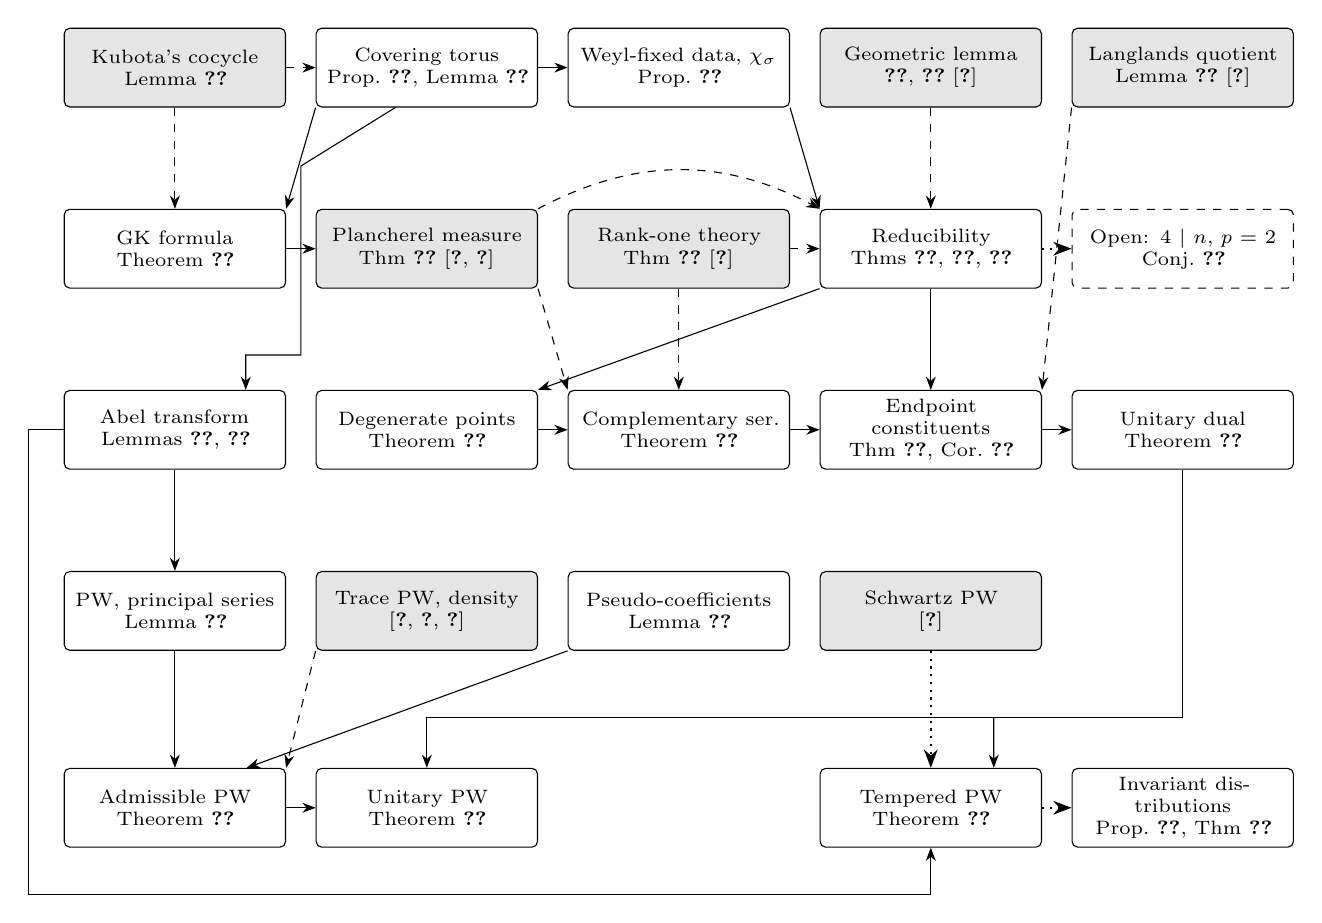
\begin{tikzpicture}[>=Stealth,
  box/.style={draw,rounded corners=2pt,align=center,font=\scriptsize,inner sep=3pt,text width=2.6cm,minimum height=1.0cm},
  lit/.style={box,fill=black!10},
  cnj/.style={box,dashed}]
% row A: structure and general inputs
\node[lit] (cocycle) at (0,0) {Kubota's cocycle\\ Lemma~\ref{lem:kubota}};
\node[box] (torus) at (3.2,0) {Covering torus\\ Prop.~\ref{prop:center}, Lemma~\ref{lem:SvN}};
\node[box] (wfix) at (6.4,0) {Weyl-fixed data, $\chi_\sigma$\\ Prop.~\ref{prop:Wfixed}};
\node[lit] (geom) at (9.6,0) {Geometric lemma\\ \ref{lem:geometric}, \ref{prop:hom} \cite{KS23}};
\node[lit] (lq) at (12.8,0) {Langlands quotient\\ Lemma~\ref{lem:langlands} \cite{BJ13}};
% row B: analytic inputs and reducibility
\node[box] (gk) at (0,-2.3) {GK formula\\ Theorem~\ref{thm:GK}};
\node[lit] (pl) at (3.2,-2.3) {Plancherel measure\\ Thm~\ref{thm:plancherel} \cite{GS16,Sz19}};
\node[lit] (r1) at (6.4,-2.3) {Rank-one theory\\ Thm~\ref{thm:rankone} \cite{He25}};
\node[box] (red) at (9.6,-2.3) {Reducibility\\ Thms~\ref{thm:n-even}, \ref{thm:n-odd-conj}, \ref{thm:reducibility}};
\node[cnj] (wild) at (12.8,-2.3) {Open: $4\mid n$, $p=2$\\ Conj.~\ref{conj:wild4}};
% row C: classification
\node[box] (abel) at (0,-4.6) {Abel transform\\ Lemmas~\ref{lem:orbital-image}, \ref{lem:ps-character}};
\node[box] (detj) at (3.2,-4.6) {Degenerate points\\ Theorem~\ref{thm:detJ}};
\node[box] (comp) at (6.4,-4.6) {Complementary ser.\\ Theorem~\ref{thm:complementary}};
\node[box] (spec) at (9.6,-4.6) {Endpoint constituents\\ Thm~\ref{thm:special}, Cor.~\ref{cor:count-special}};
\node[box] (udual) at (12.8,-4.6) {Unitary dual\\ Theorem~\ref{thm:unitary-dual}};
% row D: harmonic analysis inputs
\node[box] (pwps) at (0,-6.9) {PW, principal series\\ Lemma~\ref{lem:PWps}};
\node[lit] (bdk) at (3.2,-6.9) {Trace PW, density\\ \cite{BDK86,Li14,Li12}};
\node[box] (pseudo) at (6.4,-6.9) {Pseudo-coefficients\\ Lemma~\ref{lem:pseudo}};
\node[lit] (li) at (9.6,-6.9) {Schwartz PW\\ \cite{Li12}};
% row E: Paley-Wiener theorems
\node[box] (pwad) at (0,-9.4) {Admissible PW\\ Theorem~\ref{thm:PWad}};
\node[box] (pwu) at (3.2,-9.4) {Unitary PW\\ Theorem~\ref{thm:PWu}};
\node[box] (pwt) at (9.6,-9.4) {Tempered PW\\ Theorem~\ref{thm:PWt}};
\node[box] (dist) at (12.8,-9.4) {Invariant distributions\\ Prop.~\ref{prop:dual}, Thm~\ref{thm:FT-dist}};
% arrows, rows A-B
\draw[->,dashed] (cocycle)--(torus);
\draw[->] (torus)--(wfix);
\draw[->,dashed] (cocycle)--(gk);
\draw[->] (torus.south west)--(gk.north east);
\draw[->] (gk)--(pl);
\draw[->,dashed] (pl.north east) to[bend left=28] (red.north west);
\draw[->,dashed] (r1)--(red);
\draw[->] (wfix.south east)--(red.north west);
\draw[->,dashed] (geom)--(red);
\draw[->,dotted,thick] (red)--(wild);
% rows B-C
\draw[->] (red)--(spec);
\draw[->] (red.south west)--(detj.north east);
\draw[->,dashed] (r1)--(comp);
\draw[->,dashed] (pl.south east)--(comp.north west);
\draw[->,dashed] (lq.south west)--(spec.north east);
\draw[->] (detj)--(comp);
\draw[->] (comp)--(spec);
\draw[->] (spec)--(udual);
\draw[->] ($(torus.south)+(-0.4,0)$) -- (1.6,-1.25) -- (1.6,-3.65) -- (0.9,-3.65) -- ($(abel.north)+(0.9,0)$);
% rows C-E
\draw[->] (abel)--(pwps);
\draw[->] (pwps)--(pwad);
\draw[->,dashed] (bdk.south west)--(pwad.north east);
\draw[->] (pseudo.south west)--($(pwad.north east)+(-0.5,0)$);
\draw[->] (pwad)--(pwu);
\draw[->] (udual.south) |- (3.2,-8.25) -- (pwu.north);
\draw[->] (10.4,-8.25) -- ($(pwt.north)+(0.8,0)$);
\draw[->,dotted,thick] (li)--(pwt);
\draw[->] (abel.west) -- ++(-0.45,0) |- (9.6,-10.5) -- (pwt.south);
\draw[->,dotted,thick] (pwt)--(dist);
\end{tikzpicture}
\caption{Logical dependencies.  Shaded boxes are results taken from the literature.  The
dashed box is open.  Solid arrows are deductions made in this paper, dashed arrows use a
cited result, and dotted arrows are conditional.}\label{fig:deps}
\end{figure}

\begin{example}\label{ex:dependency}
To see how the diagram is used, consider condition (U4) of Theorem~\ref{thm:PWu} for
$F=\Q_7$, $n=3$.  It needs the location of the endpoint (Theorem~\ref{thm:detJ}), which
comes from the Plancherel measure and the rank-one theory.  It needs the unitarity of
$\pi_{nt}$ (Theorem~\ref{thm:special}).  And it needs the additivity of the trace, which
is elementary.  The surjectivity statement in Theorem~\ref{thm:PWu}(c) needs in addition
the theorem of \cite{BDK86} for covers.
\end{example}

%======================================================================
\section{Worked examples and special cases}\label{sec:examples}

This section works out the results in five cases.  The linear group serves as a
consistency check.  The double cover and two tame covers of higher degree illustrate the
two reducibility patterns.  The last subsection contrasts tame and wild covers.

\subsection{\texorpdfstring{The linear group: $n=1$}{The linear group: n=1}}

Let $n=1$.  Then $\nu=1$, $\bG=SL(2,F)$, $\bZ=\bA=A$, every $\sigma$ is a character $\chi$ of
$F^\times$ through $h$, $d_\sigma=1$ and $\chi_\sigma=\chi$.  We check each main result
against the classical theory.
\begin{itemize}[leftmargin=*,itemsep=1pt]
\item Proposition~\ref{prop:Wfixed}: $\chi^w=\chi^{-1}$, so the Weyl-fixed characters are the
quadratic characters, $[F^\times:F^{\times2}]$ in number.
\item Theorem~\ref{thm:GK}: $c(\chi)=(1-q^{-1}X)/(1-X)$ with $X=\chi(\vp)$, the classical
formula for $SL(2,F)$.
\item Theorem~\ref{thm:reducibility}: $I(\chi)$ is reducible exactly for
$\chi=|\cdot|^{\pm1}$ and for the nontrivial quadratic characters.
\item Theorem~\ref{thm:complementary}: the complementary series is $I(|\cdot|^s)$, $0<s<1$.
\item Theorem~\ref{thm:special}: at $s=1$ the kernel of $T$ is the Steinberg representation
and the image is the trivial representation, which is spherical and finite-dimensional.
\item Theorem~\ref{thm:PWad}: this is the theorem of \cite{BDK86} for $SL(2,F)$.  The
separation property is shown by explicit functions in Example~\ref{ex:EP}.
\end{itemize}

\begin{example}[A trace transform computed in full]\label{ex:macdonald}
Let $n=1$, $p$ odd, and let $f_m$ be the characteristic function of $Kh(\vp^m)K$, $m\ge1$.
On the unramified orbit, with $X=\chi(\vp)$,
\[
\hat f_m^{\,ind}(X)=P_m(X)=q^m\Bigl(\sum_{|j|\le m}X^j-q^{-1}\sum_{|j|<m}X^j\Bigr).
\]
This is Macdonald's formula $P_m(X)=q^m\bigl(X^mc(X^{-1})+X^{-m}c(X)\bigr)$.  On the
irreducible dual the function $\hat f_m$ is as follows.  At an irreducible $I(\chi)$ it is
$P_m(X)$.  At the trivial representation it is the number of cosets in $Kh(\vp^m)K/K$,
which is $q^{2m-1}(q+1)$.  At the Steinberg representation it is $0$, because that
representation has no $K$-fixed vector.  Condition (PW2) at the reducible point $X=q$
requires $P_m(q)=q^{2m-1}(q+1)+0$.  Indeed
$P_m(q)=q^m\bigl(\frac{q^{m+1}-q^{-m}}{q-1}-\frac{q^{m}-q^{-m+1}}{q(q-1)}\bigr)=q^{2m-1}(q+1)$.
At $X=-1$ the value $P_m(-1)=(-1)^mq^m(1+q^{-1})$ is the value at $\pi^+$, and the value at
$\pi^-$ is $0$.  These identities are verified in \texttt{spherical\_trace\_check.py}.
\end{example}

\subsection{\texorpdfstring{The double cover: $n=2$}{The double cover: n=2}}

Let $n=2$.  Then $\nu=1$, so $\bA$ is abelian and $\bZ=\bA$.  The genuine representations of
$\bA$ are the genuine characters $\omega$, and $d_\sigma=1$.  By Example~\ref{ex:chi-n2},
$\chi_\omega(a)=\omega(h(a^2),1)$.

\emph{Tame case, $p$ odd.}  The Weyl-fixed genuine characters are the solutions of
$\omega^2=\kappa$, that is, $\omega(h(a),1)^2=(-1,a)_2$.  There are four, and all have
$\chi_\omega=1$ (Proposition~\ref{prop:Wfixed}).  Every unitary principal series is
irreducible (Theorem~\ref{thm:moen-even}).  The orbits have coordinate $z=q^{-s}$ and
$X=\chi_\sigma(\vp)$ is a constant multiple of $z^2$.  On an orbit through a Weyl-fixed
point, with that point at $z=1$, we have $X=z^2$ and
\[
c(\sigma)c(\sigma^w)=\frac{(1-q^{-1}z^2)(1-q^{-1}z^{-2})}{(1-z^2)(1-z^{-2})}.
\]
The reducible points are $z=\pm q^{\pm1/2}$, that is, $s=\pm1/2$ relative to either of the
two Weyl-fixed points $z=\pm1$ of the orbit.  There are two such orbits, four
complementary series $0<s<1/2$, four special representations and four representations
$\pi_{nt}$.  For the unramified data the representations $\pi_{nt}$ are even Weil
representations and are spherical \cite{Ge76}.  The right half of Figure~\ref{fig:dual}
is the picture.

\emph{Wild case, $p=2$.}  The torus is still abelian.  By Lemma~\ref{lem:splittings}(e) the
center of $\bG$ is cyclic of order $4$ exactly when $(-1,-1)_2=-1$, for example for
$F=\Q_2$.  There are $[F^\times:F^{\times2}]=4\cdot2^{[F:\Q_2]}$ Weyl-fixed characters, so
eight for $\Q_2$.  The cover does not split over $K$, so there is no spherical vector and
Theorem~\ref{thm:GK} does not apply.  Theorem~\ref{thm:n-even} still gives the
irreducibility of all unitary principal series, since $n\equiv2\pmod4$.

\begin{example}\label{ex:PW-n2}
For $n=2$ and $p$ odd, Corollary~\ref{cor:PWad-explicit} reads as follows on a Weyl-stable
orbit with a Weyl-fixed point at $z=1$.  A function $h$ on the constituents is in
$PW_{ad}(\bG)$ if and only if there is a Laurent polynomial $P$ with $P(z)=P(z^{-1})$ such
that $h(I(\sigma_z))=P(z)$ for $z\ne\pm q^{\pm1/2}$,
$h(\pi_{sp}^+)+h(\pi_{nt}^+)=P(q^{-1/2})$ and $h(\pi_{sp}^-)+h(\pi_{nt}^-)=P(-q^{-1/2})$.
Here the superscripts label the two endpoints.  The space of such $h$ is the space of
symmetric Laurent polynomials plus two free parameters.
\end{example}

\subsection{\texorpdfstring{The cubic cover of $SL(2,\Q_7)$}{The cubic cover of SL(2,Q7)}}

Let $F=\Q_7$ and $n=3$, so $q=7$ and $\nu=3$.
\begin{itemize}[leftmargin=*,itemsep=1pt]
\item \emph{Torus.}  $[\bA:\bZ]=9$, $d_\sigma=3$, and $C_0=7^{\Z}\{\pm1\}(1+7\Z_7)$
(Examples~\ref{ex:torus-Q7} and \ref{ex:sigma-Q7}).
\item \emph{Weyl-fixed data.}  Four classes $\sigma_\theta$, with $\chi_{\sigma_\theta}=\theta$
quadratic (Example~\ref{ex:red-Q7}).
\item \emph{Spherical vector.}  For unramified $\sigma=\sigma_1\otimes\eta_s$ we have
$X=7^{-3s}$ and $c(\sigma)=(1-7^{-1-3s})/(1-7^{-3s})$.  In the proof of
Theorem~\ref{thm:GK} the contribution of the shell $v(x)=-m$ is the average over
$u\in\mathbb F_7^\times$ of $(u,7)_3^{-m}$, a cubic character.  It is $1$ for $3\mid m$ and
$0$ otherwise.
\item \emph{Reducibility.}  $I(\sigma_1\otimes\eta_s)$ is reducible exactly at $s=\pm1/3$
modulo $2\pi i/(3\ln7)$.  $I(\sigma_\theta)$ is reducible for the three nontrivial $\theta$.
\item \emph{Complementary series.}  $I(\sigma_1\otimes\eta_s)$, $0<s<1/3$.  At $s=1/3$ we
have $X=1/7$ and $c(\sigma)=8/7\ne0$, so the spherical vector survives in $\pi_{nt}$.
\item \emph{Discrete series.}  One special representation, and the cuspidal
representations, among them the depth-zero ones of Example~\ref{ex:depth-zero}.
\end{itemize}

\begin{example}[The Paley--Wiener conditions for $e_K$]\label{ex:PW-Q7}
Let $f=e_K$.  By Example~\ref{ex:trace-eK}, $\hat f^{\,ind}$ is $1$ on the unramified
orbit and $0$ on the others.  The values of $\hat f$ on the irreducible dual are
$\dim\pi^{K^*}$.  So $\hat f$ is $1$ at each irreducible unramified $I(\sigma)$, including
the complementary series.  At the endpoint $s=1/3$ it is $0$ at $\pi_{sp}$ and $1$ at
$\pi_{nt}$, in accordance with (U4).  At the unitary reducible point
$\sigma_{\theta_{ur}}$, where $z=-1$, exactly one of $\pi^\pm$ has a $K^*$-fixed vector, and
the values are $1$ and $0$.  On the other Weyl-stable orbit and on the cuspidal
representations $\hat f$ vanishes.  All conditions of Definition~\ref{def:PWu} hold with
$P=1$.
\end{example}

\subsection{\texorpdfstring{The quartic cover of $SL(2,\Q_5)$}{The quartic cover of SL(2,Q5)}}

Let $F=\Q_5$ and $n=4$.  Then $4\mid q-1$, so $\mu_4\subset\Q_5$, and $\nu=2$.  The center of
$\bA$ lies over $h(\Q_5^{\times2})$, of index $4$, and $d_\sigma=2$.  The group
$C_0=5^{\Z}\Z_5^{\times2}$ gives a maximal abelian subgroup of index $2$.  There are four
Weyl-fixed classes, all with $\chi_\sigma=1$.  The orbit coordinate is $z=5^{-2s}$ and
$X=5^{-4s}=z^2$ at an unramified Weyl-fixed base point.  All unitary principal series are
irreducible.  The reducible points are $s=\pm1/4$, that is, $z=\pm5^{\pm1/2}$.  There are
four special representations.  The picture is again the right half of
Figure~\ref{fig:dual}.  Note that the reducibility point $s=1/n=1/4$ is not $1/\nu$.  The
terms with $m\equiv2\pmod4$ in the proof of Theorem~\ref{thm:GK} vanish because
$u\mapsto(u,5)_4^{-2}$ is the nontrivial quadratic character of $\mathbb F_5^\times$, even
though $\hl(5^2)$ lies in the center of $\bA$.

\subsection{Tame and wild covers}

The following table contrasts the two cases.  Recall $\nu=p^rd$ with $p\nmid d$.

\begin{center}\small
\begin{tabular}{@{}>{\raggedright}p{4.2cm}>{\raggedright}p{5.2cm}>{\raggedright\arraybackslash}p{5.6cm}@{}}
\toprule
 & \textbf{Tame, $p\nmid n$} & \textbf{Wild, $p\mid n$}\\
\midrule
Center of $\bA$ & over $h(F^{\times\nu})$ & over $h(F^{\times\nu})$\\
$[\bA:\bZ]$ & $\nu^2$ & $\nu^2q^{er}$\\
$d_\sigma$ & $\nu$ & $\nu\,q^{er/2}$\\
$C_0=\vp^{\Z}\OF^{\times\nu}$ & maximal isotropic & isotropic, index $\nu q^{er}$, not maximal if $r\ge1$\\
Splitting over $K$ & yes (Kubota) & no in general\\
Weyl-fixed classes & $4$ ($p$ odd) & $4\,|2|_F^{-1}$\\
Spherical vector, $c(\sigma)$ & Theorem~\ref{thm:GK} & not available\\
Unitary reducibility & Theorems~\ref{thm:n-even}, \ref{thm:n-odd-conj} & known unless $4\mid n$\\
Plancherel measure & \cite{GS16} & \cite{Sz19} for $4\nmid n$\\
Endpoint $s=1/n$ & Theorem~\ref{thm:detJ} & expected, see below\\
Paley--Wiener (principal series) & Lemma~\ref{lem:PWps} for $p\nmid2n$ & necessity only\\
\bottomrule
\end{tabular}
\end{center}

\begin{example}[Three wild covers]\label{ex:wild}
(1) $F=\Q_2$, $n=2$.  Here $\nu=1$ and $\bA$ is abelian.  The center of $\bG$ is cyclic of
order $4$ because $(-1,-1)_2=-1$.  There are $8$ Weyl-fixed characters.

(2) $F=\Q_3(\omega)$, $n=3$.  Here $q=3$, $e=2$, $r=1$.  Then $[\OF^\times:\OF^{\times3}]=27$,
$[F^\times:F^{\times3}]=81$, $d_\sigma=9$, and $C_0$ has index $27$.  A maximal isotropic
subgroup has index $9$, and one of them contains $C_0$ with index $3$.  There are $4$ Weyl-fixed
classes, and exactly three of them give reducible unitary principal series
(Theorem~\ref{thm:n-odd-conj}).

(3) $F=\Q_2(i)$, $n=4$.  Here $q=2$, $e=2$, $\nu=2$, $r=1$.  Then
$[\OF^\times:\OF^{\times2}]=8$, $[F^\times:F^{\times2}]=16$, $d_\sigma=4$, and $C_0$ has index
$8$.  There are $16$ Weyl-fixed classes.  This is the smallest instance of the open case
of Conjecture~\ref{conj:wild4}.

The indices are computed by \texttt{wild\_torus\_check.py}.
\end{example}

\begin{remark}[The endpoint in the wild case]\label{rem:wild-endpoint}
Let $n\not\equiv0\pmod4$ and let $\sigma_0$ be Weyl-fixed with $\chi_{\sigma_0}=1$.  The proof
of Theorem~\ref{thm:reducibility} uses only Theorem~\ref{thm:plancherel} for unramified
$\chi_\sigma$ and Theorem~\ref{thm:rankone}, both of which hold without tameness.  So
$I(\sigma_0\otimes\eta_s)$ is reducible at $s=\pm1/n$ and has a complementary series for
$0<s<1/n$ also when $p\mid n$.  This depends on the identification of $\chi_\sigma$ with
the character used in \cite{Sz19}, which we did not verify in the wild case.
\end{remark}

%======================================================================
\section{Connections with related manuscripts}\label{sec:connections}

This section relates the paper to the companion manuscripts in the same project and
says which of their results are used here.

\paragraph{The unitary dual manuscript \cite{JoUD}.}  It treats the covering torus, the
split orbital integrals and the characters of principal series for $p\nmid2n$.  Its
theorem on the image of the split orbital integral is our Lemma~\ref{lem:orbital-image}(1),
and its proof is reproduced there in outline.  It also proves a matching of split-torus
traces between $\bG$ and $SL(2,F)$ when $n$ is odd or divisible by $4$.  In our terms this
matching is related to the map $\sigma\mapsto\chi_\sigma$ on principal-series parameters.
The precise comparison was not carried out here.

\paragraph{The synthesis manuscript \cite{JoSyn}.}  This is the other revision path of
the 1994 notes, combined with the $SL(2)$ part of \cite{Jo01}.  Four of its results are
incorporated here after independent verification: the vanishing of orbital integrals off
the center (Lemma~\ref{lem:vanish}), the Hermitian pairing that replaces the bilinear one
(Lemma~\ref{lem:hermitian}), the identification of the kernel and the image of the
endpoint operator (Theorem~\ref{thm:special}(a),(b)), and the algebraic factorization of
invariant distributions through the trace transform (Theorem~\ref{thm:PWad}(d) and the
remark after Proposition~\ref{prop:factor}).  That manuscript left open the normalization
of the endpoint and the exceptional datum in Moen's theorem.  Both are settled here by
Theorem~\ref{thm:GK} and Proposition~\ref{prop:Wfixed}.

\paragraph{Depth-zero characters \cite{JoCh}.}  For $n$ odd and $p\nmid2n$ that manuscript
computes the characters of depth-zero supercuspidal representations of $\bG$ on the
unramified elliptic tori and proves the relation
$\Theta_{\tilde\pi}(s(t^n))=\Theta_\pi(t)$ with the corresponding representation $\pi$ of
$SL(2,F)$.  The $n$-th power map $t\mapsto s(t^n)$ on the elliptic torus is the counterpart
of the map $s_n$ of Lemma~\ref{lem:power} on the split torus, which defines $\chi_\sigma$.
These characters give the values of the trace transform on part of the cuspidal
spectrum, which Theorem~\ref{thm:PWad} treats only through pseudo-coefficients.

\paragraph{The trace formula manuscript \cite{JoTr}.}  It develops Arthur's trace formula
for the double cover of $SL(2)$ over a number field.  The local inputs of the invariant
trace formula are the trace Paley--Wiener theorems and the density of characters.  For
$n=2$ these are Theorems~\ref{thm:PWad} and \ref{thm:PWt}, with the explicit description of
Example~\ref{ex:PW-n2}.  For general covers the invariant trace formula is due to Li
\cite{Li14}.

\paragraph{The metaplectic Jacquet--Langlands project \cite{JoMJL}.}  It concerns covers
of $GL(r)$ and of division algebras.  The link with the present paper is the restriction
from a cover of $GL(2)$ to $\bG$ (Lemma~\ref{lem:restriction}), which is the natural way
to organize the cuspidal spectrum of $\bG$ into packets.

\paragraph{Earlier papers of the author.}  The correspondence of Hecke algebras
\cite{Jo98} and of supercuspidal representations \cite{Jo99} between $\bG$ and $SL(2,F)$
for $p\nmid n$ are instances of the same comparison.  The article \cite{Jo01} contains
the invariant-distribution argument for covers of $GL(r)$ and $SL(2)$ in its original
form.

\begin{example}\label{ex:connections}
For $F=\Q_7$ and $n=3$ the comparison reads as follows.  On the split side, the genuine
principal series $I(\sigma)$ corresponds to the principal series $I(\chi_\sigma)$ of
$SL(2,\Q_7)$, and reducibility is preserved (Theorem~\ref{thm:reducibility}).  On the
elliptic side, the depth-zero supercuspidal representations correspond by \cite{JoCh}.
Whether the two correspondences fit into a single character identity is
Problem~\ref{prob:shimura}.
\end{example}

%======================================================================
\section{Open problems and future directions}\label{sec:open}

This section lists the problems that this revision leaves open.  For each we give the
formulation, the obstruction, the known results, possible approaches and the consequences.

\begin{conjecture}[Unitary principal series, wild case with $4\mid n$]\label{conj:wild4}
Let $4\mid n$ and $p=2$, with $\mu_n\subset F$.  Then $I(\sigma)$ is irreducible for every
$\sigma\in\Pi_u(\bA)$.
\end{conjecture}
\emph{Obstruction.}  The Plancherel measure is not known in this case.  The method of
\cite{GS16} uses the splitting over $K$, and the method of \cite{Sz19} excludes $4\mid n$.
\emph{Known.}  The tame case, and $n\equiv2\pmod4$.  By Theorem~\ref{thm:rankone} and
Proposition~\ref{prop:Wfixed} the conjecture is equivalent to $\mu(\sigma)=0$ for each of
the $[F^\times:F^{\times2}]$ Weyl-fixed classes.  \emph{Approaches.}  Extend the local
coefficients matrix of \cite{Sz19} to $4\mid n$.  Or use a global argument as in
\cite[Theorem~5.7]{Sz19}.  Or compute the genuine Hecke algebra as in \cite{Ka21}.
\emph{Consequences.}  The tempered dual for all $n$ and $p$ up to the cuspidal spectrum,
and the index set $\mathcal J$ of Theorem~\ref{thm:PWt}.  The smallest case is $F=\Q_2(i)$,
$n=4$ (Example~\ref{ex:wild}).

\begin{problem}[Explicit maximal abelian subgroups in the wild case]\label{prob:lagrangian}
For $p\mid\nu$ describe a subgroup $C\supset F^{\times\nu}$ of $F^\times$ that is its own
orthogonal complement for $(a,b)_n^2$, and the least $m_0$ in
Lemma~\ref{lem:splittings}(c).
\end{problem}
\emph{Obstruction.}  The wild Hilbert symbol on the unit filtration requires an explicit
reciprocity law \cite{Se81}.  \emph{Known.}  Existence and the index
$\nu|\nu|_F^{-1/2}$ (Proposition~\ref{prop:center}).  The subgroup $C_0$ is isotropic but
too small.  A Lagrangian decomposition is constructed in \cite[Lemma~2.3]{Sz19}.
\emph{Approaches.}  Use the formula of Artin--Hasse--Iwasawa for the symbol on principal
units.  \emph{Consequences.}  Explicit models of $\sigma$ and of $I(\sigma)$, needed for any
computation with $K$-types in the wild case.

\begin{problem}[The trace Paley--Wiener theorem for covers]\label{prob:BDK}
Give a written proof of the theorem of \cite{BDK86} for finite central extensions.  For
$\bG$, prove the separation property stated after Theorem~\ref{thm:PWad} directly.
\end{problem}
\emph{Obstruction.}  The proof in \cite{BDK86} uses the Bernstein center and a
decomposition theorem.  Each step has to be checked for covers.  For $\bG$ the missing
functions are analogs of the Euler--Poincar\'e function and of $e_K-e_{K'}$ in
Example~\ref{ex:EP}.  On a cover the two maximal compact subgroups carry splittings that
may differ on the Iwahori subgroup by a character.  \emph{Known.}  Part (b) of
Theorem~\ref{thm:PWad}.  The matrix Paley--Wiener theorem \cite[Appendix~A]{He25}.
\emph{Approaches.}  Use the genuine Iwahori--Hecke algebra \cite{GGK24} on the unramified
component and types on the others.  Or take traces in the matrix Paley--Wiener theorem.
\emph{Consequences.}  Theorems~\ref{thm:PWad}(c) and \ref{thm:PWu}(c) would become
independent of the statement in \cite{Li14}.

\begin{problem}[The Schwartz-space theorem]\label{prob:schwartz}
Prove Theorem~\ref{thm:PWt}(b),(c) for $\bG$ directly, including the topology, and remove
the conditions from Theorem~\ref{thm:FT-dist}.
\end{problem}
\emph{Obstruction.}  One has to verify the hypotheses admitted in \cite{Li12} in rank one
and to match Li's spaces with Definition~\ref{def:PWt}.  The kernel statement needs an
argument at the Weyl-fixed points.  \emph{Known.}  Necessity.  The rank-one $R$-group
statement \cite{He25,Lu20}.  \emph{Approaches.}  Wave packets on each circle, as in
\cite{Ar94} for linear groups.  \emph{Consequences.}  An unconditional description of all
invariant tempered distributions on $\bG$.

\begin{problem}[Moen's determinant formulas]\label{prob:moen}
Verify Propositions~\ref{prop:moen-J} and \ref{prop:moen-det} and relate $J_\mu$ to the
local coefficients matrix of \cite{Sz19,GSS23}.
\end{problem}
\emph{Obstruction.}  The preprint \cite{MoND} is not available, and the notation is not
recoverable from the 1994 text.  \emph{Known.}  The scalar $T_{\sigma^w}T_\sigma$
(Theorem~\ref{thm:plancherel}).  Determinants of local coefficients matrices are studied
in \cite{GSS23}.  \emph{Approaches.}  Compute $J_\mu$ in the model $K(\mu)$ from the
functional equations \cite[Theorems~2.1, 2.2]{GS16}.  \emph{Consequences.}  An explicit
positive definite matrix in Theorem~\ref{thm:complementary}.

\begin{problem}[Characters on the elliptic set]\label{prob:characters}
Compute the characters of $\pi^\pm$, $\pi_{sp}$ and $\pi_{nt}$ on the elliptic tori of
$\bG$.
\end{problem}
\emph{Obstruction.}  The elliptic tori of $\bG$ and their good elements must be described
first.  \emph{Known.}  The sum $\Theta_{\pi^+}+\Theta_{\pi^-}$ and
$\Theta_{\pi_{sp}}+\Theta_{\pi_{nt}}$ (Lemma~\ref{lem:ps-character}).  The depth-zero
supercuspidal characters \cite{JoCh}.  \emph{Approaches.}  Fixed points on the tree, as in
\cite{JoCh}.  The orthogonality relations of \cite[Remarque~5.8.11]{Li12}.
\emph{Consequences.}  The ellipticity statements of the 1994 Conjecture 3.16, and explicit
orbital-integral formulas for pseudo-coefficients.

\begin{problem}[The cuspidal spectrum]\label{prob:cuspidal}
Classify the genuine cuspidal representations of $\bG$ for all $n$ and $p$.  Determine
the multiplicity $m$ and the number $M$ in Lemma~\ref{lem:restriction}.
\end{problem}
\emph{Obstruction.}  Types for covers are known only in special cases.  \emph{Known.}
$n=2$ \cite{GPS83}.  Depth zero for $n$ odd \cite{JoCh}.  The correspondence \cite{Jo99}
for $p\nmid n$.  Restriction of principal series \cite{GSS26}.  \emph{Approaches.}  Types,
or restriction from covers of $GL(2)$.  \emph{Consequences.}  The first summand of
Corollary~\ref{cor:PWad-explicit} would be explicit, and the Plancherel formula would be
complete.

\begin{problem}[A local Shimura correspondence for cocenters]\label{prob:shimura}
For $p\nmid2n$ construct an isomorphism between $PW_{ad}(\bG)$ and the Paley--Wiener
space of $SL(2,F)$ for $n$ odd, or of $PGL(2,F)$ for $n$ even, at least on the
principal-series components.
\end{problem}
\emph{Obstruction.}  On the split side the map $\sigma\mapsto\chi_\sigma$ is not injective
on orbits for $n$ even, and the constituents at reducible points must be matched.
\emph{Known.}  The reducibility patterns agree (Example~\ref{ex:two-pictures}).  Split
traces match for $n$ odd or $4\mid n$ \cite{JoUD}.  Hecke algebra isomorphisms
\cite{Jo98,GGK24}.  \emph{Approaches.}  Combine the Hecke algebra isomorphisms with
Theorem~\ref{thm:PWad}.  \emph{Consequences.}  A transfer of invariant distributions
between $\bG$ and a linear group.

\begin{problem}[The global application]\label{prob:global}
Carry out the program of the 1994 manuscript: verify the local hypotheses of the invariant
trace formula for the $n$-fold cover of $SL(2,\mathbb A_k)$ and compare with $SL(2)$.
\end{problem}
\emph{Known.}  The invariant trace formula for covers \cite{Li14}.  The case $n=2$
\cite{JoTr}.  \emph{Consequences.}  A comparison of trace formulas would relate genuine
automorphic representations of the cover to automorphic representations of $SL(2)$ or
$PGL(2)$.

\begin{example}\label{ex:open}
A concrete test case for Problem~\ref{prob:BDK} is $F=\Q_7$, $n=3$, and the reducible
point $\sigma=\sigma_1\otimes\eta_{1/3}$.  One needs $f$ with $\hat f^{\,ind}=0$ and
$\Theta_{\pi_{sp}}(f)\ne0$.  A candidate is $e_K+e_{K'}-e_I$, with the idempotents formed
from the splittings over $K$, over the other maximal compact subgroup $K'$ and over the
Iwahori subgroup $I$.  It has the required property if the two splittings agree on $I$ and
the dimensions of fixed vectors are as in the table of Example~\ref{ex:EP}.
\end{example}

%======================================================================
\section{Summary of results}\label{sec:summary}

We distinguish the results by their status.

\paragraph{Proved in this paper.}  The center of the covering torus and the dimension of
its genuine representations in every residue characteristic
(Proposition~\ref{prop:center}, Lemmas~\ref{lem:C-tame}, \ref{lem:index}, \ref{lem:SvN}).
The center of $\bG$ (Lemma~\ref{lem:splittings}(e)).  The Weyl action and the $n$-th power
section (Lemmas~\ref{lem:weyl}, \ref{lem:power}).  The Weyl-fixed inducing data
(Proposition~\ref{prop:Wfixed}).  The Gindikin--Karpelevich formula in the tame case
(Theorem~\ref{thm:GK}).  The Hermitian duality of principal series
(Lemma~\ref{lem:hermitian}).  The character and the trace of principal series
(Lemma~\ref{lem:ps-character}).  The image of the trace transform on full principal series
for $p\nmid2n$ (Lemmas~\ref{lem:orbital-image}(1), \ref{lem:PWps}).  Necessity in the three
Paley--Wiener theorems, surjectivity up to the reducible points
(Theorem~\ref{thm:PWad}(a),(b)), and the bijection between the admissible and the unitary
Paley--Wiener spaces (Theorem~\ref{thm:PWu}(b)).  The dual of the tempered Paley--Wiener
space (Propositions~\ref{prop:schwartz-circle}, \ref{prop:dual}).

\paragraph{Deduced here from cited theorems.}  The reducibility of all genuine principal
series, the complementary series, the special and non-tempered representations, and the
non-cuspidal unitary and tempered duals, for $p\nmid n$
(Theorems~\ref{thm:reducibility}, \ref{thm:detJ}, \ref{thm:complementary},
\ref{thm:special}, \ref{thm:unitary-dual}).  The inputs are \cite{GS16,He25,BJ13,KS23}.

\paragraph{Cited.}  Theorems~\ref{thm:CCR}, \ref{thm:moen-even}, \ref{thm:n-even},
\ref{thm:moen-odd}, \ref{thm:n-odd-conj}, \ref{thm:plancherel}, \ref{thm:rankone}, the
surjectivity and kernel statements \ref{thm:PWad}(c),(d).

\paragraph{Conditional.}  Theorem~\ref{thm:PWt}(b),(c) and Theorem~\ref{thm:FT-dist}.

\paragraph{Open.}  Conjecture~\ref{conj:wild4} and the problems of
Section~\ref{sec:open}.

\begin{example}\label{ex:summary}
For the reader who wants one case in full: for $F=\Q_7$ and $n=3$ every statement of
Sections~\ref{sec:background} to \ref{sec:image} is either proved here or deduced from the
cited theorems, with the exception of the surjectivity in
Theorems~\ref{thm:PWad}(c), \ref{thm:PWu}(c) and \ref{thm:PWt}(b), and the kernel statement
\ref{thm:PWt}(c).
\end{example}

%======================================================================
\section*{Glossary}\addcontentsline{toc}{section}{Glossary}
\begin{description}[leftmargin=0.6cm,style=nextline,itemsep=2pt]
\item[Admissible representation] A smooth representation in which each compact open
subgroup has a finite-dimensional space of fixed vectors.
\item[Central extension, covering group] A group $\bG$ with a surjection onto $G$ whose
kernel is a finite central subgroup, here the $n$-th roots of unity.
\item[Cocenter] The quotient of a convolution algebra by the span of its commutators.
Every trace factors through it.
\item[Cocycle] A function $\beta$ on $G\times G$ with values in $\mu_n$ that defines the
multiplication $(g,\zeta)(g',\zeta')=(gg',\beta(g,g')\zeta\zeta')$ on the cover.
\item[Complementary series] Irreducible unitary representations induced from non-unitary
data.  They are not tempered.
\item[Component, orbit] An orbit is the set of twists of an inducing datum by the
characters $|a|^s$.  It is a copy of $\C^\times$.  A component of the dual is the set of
constituents of the representations induced from an orbit and its Weyl conjugate, or a
single cuspidal representation.
\item[Covering torus] The preimage in $\bG$ of the diagonal subgroup.  It is a
two-step nilpotent group, abelian only when $n\le2$.
\item[Cuspidal representation] A representation whose matrix coefficients have compact
support modulo the center.  Equivalently, its Jacquet module is zero.
\item[Genuine] A representation is genuine if a root of unity $\zeta$ in the kernel of the
cover acts by multiplication by $\zeta$.  A test function is genuine if it transforms by
$\zeta^{-1}$.
\item[Gindikin--Karpelevich formula] The formula for the scalar by which an intertwining
operator acts on the vector fixed by a maximal compact subgroup.
\item[Hermitian dual] The complex conjugate of the contragredient.  The Hermitian dual of
a genuine representation is genuine, while its contragredient in general is not.
\item[Hilbert symbol] The pairing $F^\times\times F^\times\to\mu_n$ of local class field
theory.  It is trivial exactly on pairs $(a,b)$ with $b$ a norm from $F(a^{1/n})$.
\item[Intertwining operator] A linear map between two representations that commutes with
the group actions, here the integral over the unipotent radical composed with a Weyl
element.
\item[Invariant distribution] A linear functional on test functions that takes the same
value on a function and on its conjugates.
\item[Jacquet module] The largest quotient of a representation on which the unipotent
radical acts trivially.  It is a representation of the covering torus.
\item[Langlands quotient] The unique irreducible quotient of a representation induced
from tempered data twisted into the positive chamber.
\item[Orbital integral] The integral of a test function over a conjugacy class, with a
normalizing factor.
\item[Paley--Wiener theorem] A description of the image of a Fourier transform.  For the
trace transform the image consists of functions on a set of representations.
\item[Plancherel measure] The scalar $\mu(\sigma)$ that is inverse to the composite of the
two intertwining operators attached to an inducing datum.  Its zeros and poles govern
reducibility.
\item[Principal series] The representations induced from the genuine irreducible
representations of the covering torus.
\item[Pseudo-coefficient] A test function whose trace is $1$ on one square-integrable
representation and $0$ on all other tempered irreducible representations.
\item[$R$-group] A finite group that parametrizes the constituents of a reducible
representation induced from unitary data.  Here it has order one or two.
\item[Schwartz space] The space of functions that are bi-invariant under some compact
open subgroup and decay faster than Harish-Chandra's function $\Xi$ times any power of
$1+\sigma$.
\item[Special representation] The square-integrable subrepresentation of a principal
series at the endpoint of a complementary series.  For $SL(2,F)$ it is the Steinberg
representation.
\item[Spherical vector] A vector fixed by a maximal compact subgroup over which the cover
splits.
\item[Tame, wild] The cover is tame if the residue characteristic does not divide $n$ and
wild otherwise.
\item[Tempered representation] An irreducible representation whose matrix coefficients
define continuous functionals on the Schwartz space.  The tempered representations are
those that occur in the Plancherel formula.
\item[Trace transform] The map that sends a test function $f$ to the function
$\pi\mapsto\tr\pi(f)$.
\item[Weyl-fixed] An inducing datum $\sigma$ is Weyl-fixed if conjugation by the Weyl
element gives an equivalent representation.
\end{description}

\section*{Acknowledgments}\addcontentsline{toc}{section}{Acknowledgments}
The 1994 manuscript is by David Joyner.  ChatGPT (OpenAI) prepared Draft~1 of this
revision in November 2026: it preserved the source, marked the unverified statements,
and added a section of elementary corrections.  Claude (Anthropic) prepared Draft~2 in
November 2026.  Its role was that of a reviser.  It surveyed the literature since 1994,
restated the conjectures with their present status, supplied the proofs labeled
``\proved'', wrote the verification scripts, and rewrote the exposition.  The companion
manuscripts \cite{JoUD,JoSyn,JoCh,JoTr,JoMJL} were prepared with the help of ChatGPT,
Claude and Gemini (Google), as described in their own acknowledgments.
\emph{AI review is not an independent certification of the results.}  The new proofs in
this draft have not been refereed.  Further details on the AI usage, the verification
level of each statement, and the sources that could not be consulted are in the revision
log (\texttt{revision\_log.md}).

\begin{thebibliography}{99}

\bibitem[Ar80]{Ar80} H. Arit\"urk, On the composition series of principal series
representations of a three-fold covering group of $SL(2,K)$, \emph{Nagoya Math. J.}
\textbf{77} (1980), 177--196.

\bibitem[Ar81]{Ar81} J. Arthur, The trace formula in invariant form, \emph{Ann. of Math.}
\textbf{114} (1981), 1--74.

\bibitem[Ar94]{Ar94} J. Arthur, The trace Paley--Wiener theorem for Schwartz functions,
\emph{Contemp. Math.} \textbf{177} (1994), 171--180.

\bibitem[BJ13]{BJ13} D. Ban and C. Jantzen, The Langlands quotient theorem for finite
central extensions of $p$-adic groups, \emph{Glas. Mat. Ser. III} \textbf{48} (2013),
313--334.

\bibitem[BJ16]{BJ16} D. Ban and C. Jantzen, The Langlands quotient theorem for finite
central extensions of $p$-adic groups II: intertwining operators and duality, \emph{Glas.
Mat. Ser. III} \textbf{51} (2016), 153--163.

\bibitem[Be74]{Be74} J. Bernstein, All reductive $p$-adic groups are tame, \emph{Funct.
Anal. Appl.} \textbf{8} (1974), 91--93.

\bibitem[BD84]{BD84} J. Bernstein, Le ``centre'' de Bernstein (notes by P. Deligne), in
\emph{Repr\'esentations des groupes r\'eductifs sur un corps local}, Hermann, Paris, 1984.

\bibitem[BDK86]{BDK86} J. Bernstein, P. Deligne and D. Kazhdan, Trace Paley--Wiener theorem
for reductive $p$-adic groups, \emph{J. Analyse Math.} \textbf{47} (1986), 180--192.

\bibitem[BZ76]{BZ76} J. Bernstein and A. Zelevinsky, Representations of the group
$GL(n,F)$, where $F$ is a non-Archimedean local field, \emph{Russian Math. Surveys}
\textbf{31} (1976), 1--68.

\bibitem[BZ77]{BZ77} J. Bernstein and A. Zelevinsky, Induced representations of reductive
$p$-adic groups, I, \emph{Ann. Sci. \'Ecole Norm. Sup.} \textbf{10} (1977), 441--472.

\bibitem[Bl85]{Bl85} C. Blondel, Les repr\'esentations supercuspidales des groupes
m\'etaplectiques sur $GL(2)$ et leurs caract\`eres, \emph{M\'em. Soc. Math. France}
\textbf{18}, 1985.

\bibitem[Ca95]{Ca95} W. Casselman, Introduction to the theory of admissible
representations of $p$-adic reductive groups, unpublished notes.

\bibitem[Cl91]{Cl91} L. Clozel, Invariant harmonic analysis on the Schwartz space of a
reductive $p$-adic group, in \emph{Harmonic analysis on reductive groups}, Birkh\"auser,
Boston, 1991.

\bibitem[Di77]{Di77} J. Dixmier, \emph{$C^*$-algebras}, North-Holland, Amsterdam, 1977.

\bibitem[Fe60]{Fe60} J. Fell, $C^*$-algebras with smooth dual, \emph{Illinois J. Math.}
\textbf{4} (1960), 221--230.

\bibitem[Fl80]{Fl80} Y. Flicker, Automorphic forms on covering groups of $GL(2)$,
\emph{Invent. Math.} \textbf{57} (1980), 119--182.

\bibitem[FK86]{FK86} Y. Flicker and D. Kazhdan, Metaplectic correspondence, \emph{Publ.
Math. IHES} \textbf{64} (1986), 53--110.

\bibitem[Ga23]{Ga23} F. Gao, $R$-group and Whittaker space of some genuine
representations, \emph{J. Inst. Math. Jussieu} \textbf{22} (2023).

\bibitem[GGK24]{GGK24} F. Gao, N. Gurevich and E. Karasiewicz, Genuine pro-$p$
Iwahori--Hecke algebras, Gelfand--Graev representations, and some applications, \emph{J.
Eur. Math. Soc.}, published online.

\bibitem[GSS23]{GSS23} F. Gao, F. Shahidi and D. Szpruch, Local coefficients and gamma
factors for principal series of covering groups, \emph{Mem. Amer. Math. Soc.} \textbf{283}
(2023), no.~1399.

\bibitem[GSS26]{GSS26} F. Gao, F. Shahidi and D. Szpruch, Restrictions, $L$-parameters, and
local coefficients for genuine representations, \emph{M\'em. Soc. Math. France}
\textbf{188} (2026).

\bibitem[Ge76]{Ge76} S. Gelbart, \emph{Weil's representation and the spectrum of the
metaplectic group}, Lecture Notes in Math. \textbf{530}, Springer, 1976.

\bibitem[GK82]{GK82} S. Gelbart and A. Knapp, $L$-indistinguishability and $R$ groups for
the special linear group, \emph{Adv. Math.} \textbf{43} (1982), 101--121.

\bibitem[GPS83]{GPS83} S. Gelbart and I. Piatetski-Shapiro, Some remarks on metaplectic
cusp forms and the correspondences of Shimura and Waldspurger, \emph{Israel J. Math.}
\textbf{44} (1983), 97--126.

\bibitem[GS16]{GS16} D. Goldberg and D. Szpruch, Plancherel measures for coverings of
$p$-adic $SL_2(F)$, \emph{Int. J. Number Theory} \textbf{12} (2016), 1907--1936.
arXiv:1411.6134.

\bibitem[HC70]{HC70} Harish-Chandra, \emph{Harmonic analysis on reductive $p$-adic groups}
(notes by G. van Dijk), Lecture Notes in Math. \textbf{162}, Springer, 1970.

\bibitem[He25]{He25} V. Heiermann, Sur quelques r\'esultats de Harish-Chandra pour les
repr\'esentations des groupes $p$-adiques, \'elargis aux extensions centrales, preprint,
arXiv:2506.21334, 2025.

\bibitem[Jo88]{Jo88} D. Joyner, On the metaplectic analog of Kazhdan's ``endoscopic''
lifting, \emph{Israel J. Math.} \textbf{61} (1988), 113--154.

\bibitem[Jo94a]{Jo94a} D. Joyner, A hitch-hiker's guide to invariant distributions on
$SL(2)$ over a $p$-adic field, manuscript, 1994.  Revised 2026.

\bibitem[Jo98]{Jo98} D. Joyner, A correspondence for the generalized Hecke algebra of the
metaplectic cover $\overline{SL(2,F)}$, $F$ $p$-adic, \emph{New York J. Math.} \textbf{4}
(1998), 223--235.

\bibitem[Jo99]{Jo99} D. Joyner, A correspondence for the supercuspidal representations of
$\overline{SL_2(F)}$, $F$ $p$-adic, \emph{Arch. Math.} \textbf{73} (1999), 332--340.

\bibitem[Jo01]{Jo01} D. Joyner, Invariant distributions on the $n$-fold metaplectic covers
of $GL(r,F)$, $F$ $p$-adic, \emph{J. Fourier Anal. Appl.} \textbf{7} (2001), 343--358.

\bibitem[JoCh]{JoCh} D. Joyner, Depth-zero character relations for metaplectic covers of
$SL_2$, working draft, 2026, directory \texttt{sl2bar-characters} of the repository
\texttt{github.com/wdjoyner/trace-formulas}.

\bibitem[JoMJL]{JoMJL} D. Joyner, Claude and ChatGPT, \emph{On a metaplectic
Jacquet--Langlands transfer for division algebras of prime degree}, Draft~4, 2026, in the
repository \texttt{metaplectic-jl} of the same GitHub account.

\bibitem[JoSyn]{JoSyn} D. Joyner, A hitch-hiker's guide to genuine invariant distributions
on metaplectic covers of $SL(2)$ over a $p$-adic field, Draft~3 of the synthesis with
\cite{Jo01}, 2026, directory \texttt{sl2bar-invariant-distributions} of the repository
\texttt{trace-formulas}.

\bibitem[JoTr]{JoTr} D. Joyner and Claude, A hitch-hiker's guide to the metaplectic trace
formula for $SL(2)$: basic theory, Draft~2, 2026, directory \texttt{sl2bar-trace} of the
repository \texttt{trace-formulas}.

\bibitem[JoUD]{JoUD} D. Joyner, On the unitary dual of $\overline{SL(2,F)}$, $F$ $p$-adic,
1999 manuscript, Draft~3 of the 2026 revision, directory \texttt{sl2bar-unitary-dual} of
the repository \texttt{trace-formulas}.

\bibitem[KS23]{KS23} E. Kaplan and D. Szpruch, A note on the representation theory of
central extensions of reductive $p$-adic groups, \emph{Comm. Algebra} \textbf{51} (2023),
4363--4371.

\bibitem[Ka18]{Ka18} C. Karimianpour, Branching rules for $n$-fold covering groups of
$SL_2$ over a non-Archimedean local field, \emph{Canad. Math. Bull.} \textbf{61} (2018).

\bibitem[Ka21]{Ka21} E. Karasiewicz, A Hecke algebra on the double cover of a Chevalley
group over $\Q_2$, \emph{Algebra Number Theory} \textbf{15} (2021), 1729--1753.

\bibitem[KP84]{KP84} D. Kazhdan and S. Patterson, Metaplectic forms, \emph{Publ. Math.
IHES} \textbf{59} (1984), 35--142.

\bibitem[Ku67]{Ku67} T. Kubota, Topological covering of $SL(2)$ over a local field,
\emph{J. Math. Soc. Japan} \textbf{19} (1967), 114--121.

\bibitem[Li12]{Li12} W.-W. Li, La formule des traces pour les rev\^etements de groupes
r\'eductifs connexes. II. Analyse harmonique locale, \emph{Ann. Sci. \'Ec. Norm. Sup\'er.}
\textbf{45} (2012), 787--859.  arXiv:1107.1865v3.

\bibitem[Li14]{Li14} W.-W. Li, La formule des traces pour les rev\^etements de groupes
r\'eductifs connexes. IV. Distributions invariantes, \emph{Ann. Inst. Fourier}
\textbf{64} (2014), 2379--2448.

\bibitem[Lu20]{Lu20} C. Luo, Knapp--Stein dimension theorem for finite central covering
groups, \emph{Pacific J. Math.} \textbf{306} (2020), 265--280.

\bibitem[Ma57]{Ma57} G. Mackey, Borel structure in groups and their duals, \emph{Trans.
Amer. Math. Soc.} \textbf{85} (1957), 134--165.

\bibitem[Mc12]{Mc12} P. McNamara, Principal series representations of metaplectic groups
over local fields, in \emph{Multiple Dirichlet series, $L$-functions and automorphic
forms}, Progr. Math. \textbf{300}, Birkh\"auser, 2012, 299--327.  arXiv:0911.2274.

\bibitem[MoND]{MoND} C. Moen, Intertwining operators for covering groups of $SL(2)$ over a
local field, undated preprint.

\bibitem[Mo88]{Mo88} C. Moen, Irreducibility of unitary principal series for covering
groups of $SL(2,k)$, \emph{Pacific J. Math.} \textbf{135} (1988), 89--110.

\bibitem[Mo68]{Mo68} C. Moore, Group extensions of $p$-adic and adelic linear groups,
\emph{Publ. Math. IHES} \textbf{35} (1968), 157--222.

\bibitem[Ne99]{Ne99} J. Neukirch, \emph{Algebraic number theory}, Springer, 1999.

\bibitem[Sa67]{Sa67} P. Sally, Analytic continuation of the irreducible unitary
representations of the universal covering group of $SL(2,\R)$, \emph{Mem. Amer. Math.
Soc.} \textbf{69}, 1967.

\bibitem[Sc50]{Sc50} L. Schwartz, \emph{Th\'eorie des distributions}, vol.~I, Hermann,
Paris, 1950.

\bibitem[Se81]{Se81} S. Sen, On explicit reciprocity laws II, \emph{J. Reine Angew. Math.}
\textbf{323} (1981), 68--87.

\bibitem[Se77]{Se77} J.-P. Serre, \emph{Linear representations of finite groups},
Springer, 1977.

\bibitem[Si79]{Si79} A. Silberger, \emph{Introduction to harmonic analysis on reductive
$p$-adic groups}, Princeton Univ. Press, 1979.

\bibitem[Sz19]{Sz19} D. Szpruch, On Shahidi local coefficients matrix, \emph{Manuscripta
Math.} \textbf{159} (2019), 117--159.  arXiv:1609.08122.

\bibitem[Sz24]{Sz24} D. Szpruch, Whittaker spaces for reducible unitary principal series
representations of $\widetilde{SL_2(F)}$, preprint, arXiv:2411.11460, 2024.

\bibitem[Ta83]{Ta83} M. Tadi\'c, The topology of the dual space of a reductive group over
a local field, \emph{Glas. Mat.} \textbf{18} (1983), 259--279.

\bibitem[Ta75]{Ta75} M. Taibleson, \emph{Fourier analysis on local fields}, Princeton
Univ. Press, 1975.

\bibitem[Vi81]{Vi81} M.-F. Vign\'eras, Caract\'erisation des int\'egrales orbitales sur un
groupe r\'eductif $p$-adique, \emph{J. Fac. Sci. Univ. Tokyo} \textbf{28} (1981),
945--961.

\bibitem[We75]{We75} A. Weil, \emph{Basic number theory}, 3rd ed., Springer, 1974.

\bibitem[We09]{We09} M. Weissman, Metaplectic tori over local fields, \emph{Pacific J.
Math.} \textbf{241} (2009), 169--200.

\end{thebibliography}

\end{document}
